\documentclass{article}
\AtBeginDocument{\RenewCommandCopy\qty\SI}
\usepackage{style}
\title{ECE358 Cheatsheet}
\author{John Doe}
\lhead{ECE358}
\rhead{John Doe}

\begin{document}
\maketitle

\tableofcontents

\listoffigures

\listoftables

Read the textbook for this course. 

\section{Course Tips}
\begin{intuition}
    \begin{itemize}
        \item Go to ECE345 sessions to catch up if you miss a lecture since exact same content. Tutorials do more examples. 
        \item Homeworks are more difficult than the midterm and exam.
        \item Open CLRS Book: Open book, electronic notes, and handouts are good. 
        \item Do not use AI when doing HW, as this is great practice for midterms/finals.
        \item Greedy or dynamic is always in either the midterm or exam. If greedy on the midterm, then exam will have dynamic programming. 
        \item NP completeness on the final. 
        \item Code the components to get used to it. 
    \end{itemize}
\end{intuition}

\section{Preliminaries}
\subsection{Pseudocode}
\begin{warning}
    \begin{itemize}
        \item Do not write C/Python/Java codes.
        \item Do not copy entire block of known codes (e.g. build-heap, heapsort) form textbook. You should abstract out the details.
    \end{itemize}
\end{warning}

\subsection{Exam}
\begin{warning}
    \begin{itemize}
        \item \textbf{Explanation:} Clearly explain your algorithms using English or Pseudocode + English. 
        \begin{itemize}
            \item You can reference your algorithm/comments for your proof of correctness.
        \end{itemize}
        \item \textbf{Algorithms from class:} You can assume its correctness and use it to prove other algorithms. 
        \begin{itemize}
            \item However, if you modify it, then you need to prove the new algorithm from scratch.
        \end{itemize}
        \item \textbf{Loops:} State what will happen before and after each loop execution is sufficient. 
    \end{itemize}
\end{warning}
\newpage

% W1
\section{Asymptotics (Ch. 3.1-2 pg. 50-63, L2)} 
Asymptotic efficiency focuses on understanding how the running time of an algorithm grows with the input size, particularly for large inputs.
\subsection{Big-O (Upper Bound)}
    \begin{definition} 
        $ f(n) = O(g(n)) \text{ iff } \exists \text{ positive constants } c \text{ and } n_0 \text{ s.t. } 0 \leq f(n) \leq c g(n) \; \forall \; n \geq n_0 $
        \begin{itemize}
            \item \textbf{Asymptotic upper bound:} Grows \textbf{no faster} than a certain rate, based on the highest-order term.
        \end{itemize}
    \end{definition}

    \begin{warning}
        Every function $f(n)$ in the set $O(g(n))$ must be \textbf{asymptotically nonnegative} (i.e. $f(n)$ must be positive whenever $n$ is sufficiently large).
    \end{warning}

    \begin{example}
        To show that \( 13n + 7 \in O(n) \), we need to find constants \( c > 0 \) and \( n_0 > 0 \) such that:

        \[
        13n + 7 \leq c \cdot n \quad \text{for all } n \geq n_0.
        \]

        \begin{enumerate}
            \item Start with the inequality:
            
            \[
            13n + 7 \leq c \cdot n.
            \]
            
            \item Rearrange the inequality to isolate \( c \):
            
            \[
            13n + 7 \leq c \cdot n \implies 13 + \frac{7}{n} \leq c.
            \]
            
            \item For this inequality to hold for all \( n \geq n_0 \), choose \( n_0 \) such that \( \frac{7}{n_0} \) is sufficiently small.
            
            \item Set \( n_0 = 7 \):
            
            \[
            \frac{7}{n_0} = \frac{7}{7} = 1.
            \]
            
            Now the inequality becomes:
            
            \[
            13 + \frac{7}{7} = 13 + 1 = 14 \leq c.
            \]
            
            \item Choose \( c = 14 \). This choice satisfies:
            
            \[
            13 + \frac{7}{n} \leq 14 \quad \text{for all } n \geq 7.
            \]
            
            \item Therefore, with \( c = 14 \) and \( n_0 = 7 \), we have:
            
            \[
            13n + 7 \leq 14n \quad \text{for all } n \geq 7.
            \]
        \end{enumerate}
    \end{example}

    \begin{example}
        To prove that \( \frac{1}{2}n^2 - 3n \in O(n^2) \), we need to show:

        \[
        \frac{1}{2}n^2 - 3n \leq C \cdot n^2 \quad \text{for some constants } C > 0 \text{ and } n_0 > 0 \text{, for all } n \geq n_0.
        \]

        \begin{enumerate}
            \item Start with the inequality we want to prove:
            
            \[
            \frac{1}{2}n^2 - 3n \leq C \cdot n^2.
            \]
            
            \item Rearrange the inequality to isolate \( C \):
            
            \[
            \frac{1}{2}n^2 - 3n \leq C \cdot n^2 \implies \frac{1}{2} - \frac{3}{n} \leq C.
            \]
            
            \item For the inequality to hold for all \( n \geq n_0 \), we need to make \( \frac{3}{n} \) sufficiently small:
            
            \item Set \( n_0 = 1 \). For \( n \geq 1 \):
            
            \[
            \frac{3}{n} \leq 3 \quad \Rightarrow \quad \frac{1}{2} - \frac{3}{n} \leq \frac{1}{2} - 3.
            \]
            
            However, this inequality might lead to negative values for smaller \( n \), so we adjust \( C \) accordingly.
            
            \item Choose \( C = \frac{7}{2} \). With this choice:
            
            \[
            \frac{1}{2} - \frac{3}{n} \leq C \quad \text{for all } n \geq 1.
            \]
            
            Setting \( C = 3.5 \) ensures that:
            
            \[
            \frac{1}{2} - \frac{3}{n} \leq 3.5 \quad \text{holds for all } n \geq 1.
            \]
            
            \item Therefore, with \( C = 3.5 \) and \( n_0 = 1 \), we have:
            
            \[
            \frac{1}{2}n^2 - 3n \leq 3.5n^2 \quad \text{for all } n \geq 1.
            \]
        \end{enumerate}

        This confirms that \( \frac{1}{2}n^2 - 3n \in O(n^2) \).
    \end{example}

    \begin{warning}
        The choice of $C=3.5$ was just one option. Any constant C that satisfies the inequality works. It doesn't have to be the tightest bound for big-O.
    \end{warning}

    \begin{example}
        \[
        n! = 1 \cdot 2 \cdot 3 \cdot 4 \cdot \ldots \cdot n \leq n \cdot n \cdot n \cdot \ldots \cdot n = O(n^n) \quad \text{(with \( n \) terms)}
        \]

        Similarly:

        \[
        \log n! = O(n \log n) = O(\log n^n)
        \]
    \end{example}

    \begin{example}
        \textbf{Statement:} Prove that $2^{n+1} = O(2^n)$.
        
        \textbf{Step 1:} Begin by noting that $2^{n+1}$ can be rewritten as:
        \[
        2^{n+1} = 2 \cdot 2^n
        \]
        We want to show that $2^{n+1} \leq C \cdot 2^n$ for some constant $C$ and for all $n \geq n_0$.
        
        \textbf{Step 2:} To satisfy the definition of Big-O, we need:
        \[
        0 \leq 2 \cdot 2^n \leq C \cdot 2^n \quad \forall n \geq 0
        \]
        This inequality holds if $C \geq 2$, as the factor of 2 on the left-hand side is less than or equal to $C$.
        
        \textbf{Step 3:} Let us choose $C = 3$ and $n_0 = 1$. Now check the inequality for all $n \geq n_0$:
        \[
        0 \leq 2 \cdot 2^n \leq C \cdot 2^n \quad \forall n \geq n_0
        \]
        This is true because $2 \cdot 2^n \leq 3 \cdot 2^n$ holds for all $n \geq 1$.
        
        \textbf{Conclusion:} Therefore, we have shown that:
        \[
        2^{n+1} = O(2^n)
        \]
    \end{example}
        

    \begin{example}
        \textbf{Statement:} Prove that $2^{n+1} = \Omega(2^n)$.
        
        \textbf{Step 1:} Recall the definition of $\Omega$: we need to show that $2^{n+1} \geq C \cdot 2^n$ for some constant $C > 0$ and for all $n \geq n_0$.
        
        \textbf{Step 2:} Again, we can rewrite $2^{n+1}$ as:
        \[
        2^{n+1} = 2 \cdot 2^n
        \]
        We want to show:
        \[
        0 \leq C \cdot 2^n \leq 2 \cdot 2^n \quad \forall n \geq 0
        \]
        This inequality holds if $C \leq 2$.
        
        \textbf{Step 3:} Let us choose $C = 1$ and $n_0 = 1$. Now verify the inequality:
        \[
        0 \leq C \cdot 2^n \leq 2 \cdot 2^n \quad \forall n \geq 1
        \]
        This is true because $1 \cdot 2^n \leq 2 \cdot 2^n$ holds for all $n \geq 1$.
        
        \textbf{Conclusion:} Therefore, we have shown that:
        \[
        2^{n+1} = \Omega(2^n)
        \]
    \end{example}

\subsection{Big-Omega (Lower Bound)}
    \begin{definition}
        $ f(n) = \Omega(g(n)) \text{ iff } \exists \text{ positive constants } c \text{ and } n_0 \text{ such that } 0 \leq c g(n) \leq f(n) \; \forall \; n \geq n_0 $
        \begin{itemize}
            \item \textbf{Asymptotic lower bound:} Grows \textbf{at least as fast} as a certain rate, based on the highest-order term.
        \end{itemize}
    \end{definition}

    \begin{example}
        \begin{enumerate}
            \item The sum can be approximated by considering that the sequence is bounded above by:
        
            \[
            1 + 2 + 3 + \ldots + n \geq \left\lceil \frac{n}{2} \right\rceil + \left( \left\lceil \frac{n}{2} \right\rceil + 1 \right) + \ldots + n.
            \]
        
            \item Grouping terms to form pairs around the middle:
        
            \[
                \left\lceil \frac{n}{2} \right\rceil + \left( \left\lceil \frac{n}{2} \right\rceil + 1 \right) + \ldots + n \geq \left\lceil \frac{n}{2} \right\rceil \times \left\lceil \frac{n}{2} \right\rceil = \left\lceil \frac{n^2}{4} \right\rceil
            \]
        
            \item To express this in terms of \( \Omega(n^2) \), note that:
        
            \[
            \left\lceil \frac{n^2}{4} \right\rceil \geq \frac{n^2}{4}
            \]
        
            \item This implies:
        
            \[
            \left( \frac{1}{n} \right)n^2 = \Omega(n^2)
            \]
        
            \item Finding \( n_1 \): We choose \( n_1 \) such that the inequality holds for all \( n \geq n_1 \). Let's find \( n_1 \) by ensuring:
        
            \[
            \left\lceil \frac{n^2}{4} \right\rceil \geq c \cdot n^2
            \]
        
            Choosing \( c = \frac{1}{4} \), we need \( \left\lceil \frac{n^2}{4} \right\rceil \geq \frac{n^2}{4} \). This inequality naturally holds for \( n \geq 1 \). Thus, we can choose \( n_1 = 1 \), which gives:
        
            \[
            \left\lceil \frac{n^2}{4} \right\rceil = \Omega(n^2)
            \]
        
            This satisfies the inequality for all \( n_1 \geq 1 \).
        \end{enumerate}
        
        Thus, the sum \( 1 + 2 + 3 + \ldots + n \) is \( \Omega(n^2) \), indicating a quadratic lower bound.        
    \end{example}

\subsection{Big-Theta (Tight Bound)}
    \begin{definition}
        $ f(n) = \Theta(g(n)) \text{ iff } \exists \text{ positive constants } c_1, \; c_2, \; n_0 \text{ s.t. } 0 \leq c_1 g(n) \leq f(n) \leq c_2 g(n) \; \forall \; n \geq n_0 $
        \begin{itemize}
            \item \textbf{Asymptotically tight bounds:} Grows \textbf{precisely} at a certain rate, based on the highest-order term.
        \end{itemize}
    \end{definition}

    \begin{example}
        Consider the sum \( 1 + 2 + 3 + \ldots + n \), prove that it is $\Theta(n^2)$
        \begin{enumerate}
            \item From the previous example with Big-Omega, we know that $\Omega(n^2)$
            \item The sum can be written as:

            \[
            1 + 2 + 3 + \ldots + n = \frac{n(n+1)}{2}
            \]
        
            \item Expanding the expression:
        
            \[
            = \frac{1}{2}n^2 + \frac{1}{2}n
            \]
        
            \item Therefore, this sum is:
        
            \[
            = O(n^2)
            \]
            \item By Theorem 3.1, $\Theta(n^2)$.
        \end{enumerate}
    \end{example}

    \begin{example}
        Let \( f(n) = \sum_{i=1}^n i^k \). We want to show that \( f(n) = \Omega(n^{k+1}) \) and \( f(n) = O(n^{k+1}) \), indicating that \( f(n) \) is asymptotically bounded both above and below by \( n^{k+1} \).

        \begin{enumerate}

            \item Prove that \( f(n) = O(n^{k+1}) \):
            
            \begin{enumerate}
                \item Start with the definition of \( f(n) \):
                
                \[
                f(n) = \sum_{i=1}^n i^k.
                \]
                
                \item Observe that each \( i^k \) is less than or equal to \( n^k \) for \( i \leq n \). Therefore, we can bound the sum from above:
                
                \[
                \sum_{i=1}^n i^k \leq \sum_{i=1}^n n^k = n^k + n^k + \ldots + n^k = n \cdot n^k = n^{k+1}.
                \]
                
                \item This implies:
                
                \[
                f(n) = O(n^{k+1}),
                \]
                
                where the constant \( C \) can be chosen as 1. Thus, there exists a constant \( C > 0 \) such that \( f(n) \leq C \cdot n^{k+1} \) for sufficiently large \( n \).
                
            \end{enumerate}

            \item Prove that \( f(n) = \Omega(n^{k+1}) \):
            
            \begin{enumerate}
                \item To establish a lower bound, consider using a double sequence method:
                
                \[
                2f(n) = \sum_{i=1}^n i^k + \sum_{i=1}^n (n-i+1)^k.
                \]
                
                \item Notice that the first sum is ascending (i.e., \( 1^k + 2^k + \ldots + n^k \)) and the second sum is descending (i.e., \( n^k + (n-1)^k + \ldots + 1^k \)):
                
                \[
                2f(n) = \sum_{i=1}^n i^k + \sum_{i=1}^n (n-i+1)^k.
                \]
                
                \item Each pair \( i^k + (n-i+1)^k \) is greater than or equal to \( \left(\frac{n}{2}\right)^k \):
                
                \[
                2f(n) \geq \sum_{i=1}^n \left(\frac{n}{2}\right)^k = \left(\frac{n}{2}\right)^k + \ldots + \left(\frac{n}{2}\right)^k = n \cdot \left(\frac{n}{2}\right)^k = \frac{n^{k+1}}{2^k}.
                \]
                
                \item This simplifies to:
                
                \[
                2f(n) \geq \frac{n^{k+1}}{2^k} \Rightarrow f(n) \geq \frac{n^{k+1}}{2^{k+1}}.
                \]
                
                \item Therefore:
                
                \[
                f(n) = \Omega(n^{k+1}),
                \]
                
                showing that \( f(n) \) has a quadratic lower bound.
                
            \end{enumerate}

        \end{enumerate}

        \textbf{Conclusion:} Since \( f(n) \) is bounded above and below by \( n^{k+1} \), we conclude:

        \[
        f(n) = \Theta(n^{k+1}).
        \]
    \end{example}

    \begin{example}
        Show that $(n + a)^b = \Theta(n^b)$
        \begin{enumerate}
            \item \textbf{Key Observation:}
                \[
                n + a \leq n + |a| \leq 2n \quad \text{if} \ n \geq |a|
                \]
                \[
                n + a \geq n - |a| \geq \frac{1}{2} n \quad \text{if} \ n \geq 2|a|
                \]
            
            \item $(n + a)^b = O(n^b):$
            \[
            0 \leq (n + a)^b \leq C \cdot n^b
            \]
            Let $n_0 = |a| \Rightarrow 0 \leq (n + a)^b \leq (2n)^b = 2^b n^b$.
            Therefore, let $C \geq 2^b$ and the above holds (i.e. using the key observation):
            \[
            \therefore (n + a)^b = O(n^b)
            \]

            \item $(n + a)^b = \Omega(n^b):$
            \[
            0 \leq C \cdot n^b \leq (n + a)^b
            \]
            Let $n_0 = 2|a| \Rightarrow (n + a)^b \geq \left(\frac{1}{2} n \right)^b = \left(\frac{1}{2} \right)^b n^b$.
            Therefore, let $0 < C \leq \left(\frac{1}{2}\right)^b$ and the above holds:
            \[
            \therefore (n + a)^b = \Omega(n^b)
            \]

            \item Conclusion:
            \[
            \therefore (n + a)^b = O(n^b) \quad \text{and} \quad (n + a)^b = \Omega(n^b) \Rightarrow (n + a)^b = \Theta(n^b)
            \]
            \end{enumerate}
    \end{example}

\customFigure[1]{00_Images/BigO_Omega_Theta_Notation.png}{Graphical examples of the Big-O, Big-Omega, and Big-Theta.}

\begin{intuition}
    In all asymptotic notations, you are trying to describe a function after $n_0$ (i.e. ignore all flunctuation before).
\end{intuition}

\subsection{Theorem 3.1}
    \begin{theorem}
        $f(n) = \Theta(g(n))$ iff $f(n) = O(g(n))$ and $f(n)=\Omega(g(n))$.
    \end{theorem}

\subsection{Small-O (Strictly Slower)}
\begin{definition}
    $f(n) = o(g(n)) \text{ iff } \forall c > 0, \exists n_0 > 0 \text{ s.t. } 0 \leq f(n) < c g(n) \text{ for all } n \geq n_0.$
\end{definition}

\subsection{Small-Omega (Strictly Faster)}
\begin{definition}
    $f(n) = \omega(g(n)) \text{ iff } \forall c > 0, \exists n_0 > 0 \text{ s.t. } 0 \leq c g(n) < f(n) \text{ for all } n \geq n_0.$
\end{definition}

\subsection{Asymptotic notation and running times}
    \begin{warning}
        Make sure that the asymptotic notation you use is as precise as possible without overstating which running time (i.e. worst-case, best-case, or any average/expected-case) it applies to.
    \end{warning}

\subsection{Abuses of asymptotic notation}
    \begin{intuition}
        \begin{itemize}
            \item \textbf{Equality:}
            \begin{itemize}
                \item When asymptotic notation stands alone on the RS of an equation (or inequality), then $= \text{ means } \in$.
                \item When asymptotic notation is in a formula, it is an anonymous function (AF) that we do not care to name.
                \item When asymptotic notation appears on the LS of an equation: No matter how the AF is chosen on the LS, there is a way to choose the AF on the RS to make the equation valid.
            \end{itemize}
            \item \textbf{Variable tending toward $\infty$ must be inferred from context:}
            \begin{itemize}
                \item e.g. $O(g(n))$, then we are interested in the growth of $g(n)$ as $n$ grows.
                \item e.g. $f(n) = O(1)$, then $f(n)$ is bounded from above by a constant as $n$ goes to $\infty$.
                \item e.g. $T(n) = O(1) \text{ for } n<3$ is that there exists a positive constant $c$ such that $T(n) \leq c \text{ for } n<3$.
            \end{itemize}
        \end{itemize}
    \end{intuition}

\subsection{Comparing function properties}
    \begin{definition}
        
        \textbf{Transitivity:}
        \begin{itemize}
            \item $f(n) = \Theta(g(n)) \text{ and } g(n)=\Theta(h(n)) \text{ imply } f(n) = \Theta(h(n))$
            \item $f(n) = O(g(n)) \text{ and } g(n)=O(h(n)) \text{ imply } f(n) = O(h(n))$
            \item $f(n) = \Omega(g(n)) \text{ and } g(n)=\Omega(h(n)) \text{ imply } f(n) = \Omega(h(n))$
        \end{itemize}
        \vspace{1em}

        \textbf{Symmetry:}
        \begin{itemize}
            \item $f(n) = \Theta(g(n)) \text{ iff } g(n) = \Theta(f(n))$.
        \end{itemize}
        \vspace{1em}

        \textbf{Transpose symmetry:}
        \begin{itemize}
            \item $f(n) = O(g(n)) \text{ iff } g(n) = \Omega(f(n))$
        \end{itemize}
        \vspace{1em}

        \textbf{Different functions:}
        \begin{itemize}
            \item \( n^a = O(n^b) \), iff \( a \leq b \).
            \item \( \log_a(n) = O(\log_b(n)) \), $\forall$ \( a, b \).
            \item \( c^n = O(d^n) \), iff \( c \leq d \).
            \item If \( f(n) = O(f'(n)) \) and \( g(n) = O(g'(n)) \), then:
            \begin{enumerate}
                \item \( f(n) \cdot g(n) = O(f'(n) \cdot g'(n)) \).
                \item \( f(n) + g(n) = O(\max\{f'(n), g'(n)\}) \).
                \begin{itemize}
                    \item ' is not a derivative, just another function. 
                \end{itemize}
            \end{enumerate}
        \end{itemize}
        
    \end{definition}

    \begin{intuition}
        \begin{itemize}
            \item \( 1 \ll \log^*(n) \ll \log^i n \ll (\lg n)^a \ll n^b \ll c^n \quad \forall i, a, b, c \)
            
            \item \( f(n) \ll g(n) \Rightarrow h(n)f(n) \ll h(n)g(n) \)
            
            \item \( f(n) \ll g(n) \Rightarrow f(n)^{h(n)} \ll g(n)^{h(n)} \)
            
            \item \( f(n) \ll g(n) \) and \( \lim_{n \to \infty} h(n) > 1 \Rightarrow h(n)^{f(n)} \ll h(n)^{g(n)} \)
            
            \item Assume \( f \) and \( h \) are eventually positive, i.e. \( \lim_{n \to \infty} f(n) > 0 \) and \( \lim_{n \to \infty} h(n) > 0 \). 
            \begin{itemize}
                \item Note: \( f(n) \ll g(n) \Rightarrow \lim_{n \to \infty} g(n) = \infty \)
            \end{itemize}
            
            \item \( f(n) \ll g(n) \) means \( f(n) = o(g(n)) \)
            
            \item Notice the direction of the replication.
        \end{itemize}    
    \end{intuition}

    \begin{derivation}
        In tutorial 2.
    \end{derivation}
    
        \subsubsection{Common justification steps}
        \begin{intuition}
            \begin{itemize}
                \item Exponential functions grow faster than polynomial functions, which grow faster than polylogarithmic functions.
                \item The base of a logarithm doesn’t matter asymptotically, but the base of an exponential and the degree of a polynomial do matter.
            \end{itemize}
        \end{intuition}

\subsection{Limit method}
    \begin{definition}
        Find the asymptotic relationship between two functions for which you might not have any intuition about. 
        \begin{equation}
            \lim_{n \to \infty} \frac{f(n)}{g(n)} = 0 \Rightarrow f(n) = o(g(n))
        \end{equation}
        
        \begin{equation}
            \lim_{n \to \infty} \frac{f(n)}{g(n)} = \infty \Rightarrow f(n) = \omega(g(n))
        \end{equation}
        
        \begin{equation}
            \lim_{n \to \infty} \frac{f(n)}{g(n)} < \infty \text{ i.e. is anything finite } \Leftrightarrow f(n) = O(g(n))
        \end{equation}
        
        \begin{equation}
            \lim_{n \to \infty} \frac{f(n)}{g(n)} > 0 \text{ i.e. non-zero } \Leftrightarrow f(n) = \Omega(g(n))
        \end{equation}
        
        \begin{equation}
            \lim_{n \to \infty} \frac{f(n)}{g(n)} = C \text{ s.t. } 0 < C < \infty \Leftrightarrow f(n) = \Theta(g(n))
        \end{equation}        
    \end{definition}

    \subsubsection{L'Hôpital's rule}
    \begin{definition}
        $\text{if } \lim_{x \to a} \frac{f(x)}{g(x)} = \frac{0}{0} \text{ or } \frac{\infty}{\infty}$ then,
        \begin{equation}
            \lim_{x \to c} \frac{f(x)}{g(x)} = \lim_{x \to c} \frac{f'(x)}{g'(x)}
        \end{equation}
        
    \end{definition}

    \begin{warning}
        $f(n)$ and $g(n)$ need to be different functions. 
    \end{warning}

\subsection{Polynomially-bounded}
\begin{definition}
    \begin{itemize}
        \item \textbf{Polylogarithmically bounded:} \( f(n) = O((\lg n)^k) \quad \exists k > 0 \)
        
        \item \textbf{Polynomially bounded:} \( f(n) = O(n^k) \quad \exists k > 0 \)
        
        \item \textbf{Exponentially bounded:} \( f(n) = O(k^n) \quad \exists k > 0 \)
    \end{itemize}
\end{definition}

\begin{intuition}
    \begin{itemize}
        \item \textbf{Notation:} \( (\lg n)^2 = (\lg n) \cdot (\lg n) \) (polylogarithmic) and \( \lg^2 n = \lg(\lg n) \) (iterated log). 
    \end{itemize}
\end{intuition}

\begin{theorem}
    $f(n) = O(n^k) \Leftrightarrow \lg(f(n)) = O(\lg n)$
\end{theorem}

\begin{theorem}
    All logarithmically bounded functions are polynomially bounded, i.e. \((\lg n)^a = O(n^b) \quad \forall a, b > 0\)
\end{theorem}

\begin{theorem}
    All polynomially bounded functions are exponentially bounded, i.e. \( f(n) = O(n^a) \Rightarrow f(n) = O(b^n) \quad \forall a > 0 \text{ and } \forall b > 1\)
\end{theorem}

\begin{derivation}
    In tutorial 2.
\end{derivation}

\subsection{Logarithm method}
    \begin{definition}
        \textbf{Limit of Logs:} $\lim_{x \to a} (\log_b f(x)) = \log_b \left( \lim_{x \to a} f(x) \right)$

        $\text{Suppose we want to compute } \lim_{n \to \infty} \frac{f(n)}{g(n)} = L$

        \[
        \therefore \lg \left( \lim_{n \to \infty} \frac{f(n)}{g(n)} \right) = \lg L
        \]

        \[
        \therefore \lim_{n \to \infty} \left( \lg \frac{f(n)}{g(n)} \right) = \lg L
        \]

        \[
        \therefore \lim_{n \to \infty} \frac{f(n)}{g(n)} = L = 2^{\lim_{n \to \infty} \lg \left( \frac{f(n)}{g(n)} \right)}
        \]
    \end{definition}

    \begin{example}
        \begin{enumerate}

            \item \textbf{Apply logarithm to the limit.}
            Start by taking the logarithm of the limit:
            \[
            \lg \left( \lim_{n \to \infty} \frac{2^{n+1}}{4^n} \right)
            \]
        
            \item \textbf{Move the logarithm inside the limit.}
            Since the logarithm function is continuous, we can move it inside the limit:
            \[
            \lim_{n \to \infty} \left( \lg \frac{2^{n+1}}{4^n} \right)
            \]
        
            \item \textbf{Simplify the logarithmic expression.}
            Use the properties of logarithms to break down the expression:
            \[
            \lim_{n \to \infty} \left( (n+1) \lg 2 - n \lg 4 \right)
            \]
            Since \( \lg 4 = 2 \lg 2 \), we can rewrite the expression as:
            \[
            \lim_{n \to \infty} \left( (n+1) \lg 2 - n \cdot 2 \lg 2 \right)
            \]
        
            \item \textbf{Combine the terms.}
            Simplify the terms:
            \[
            \lim_{n \to \infty} \left( (n+1) \lg 2 - 2n \lg 2 \right) = \lim_{n \to \infty} \left( \lg 2 - n \lg 2 \right)
            \]
            This simplifies to:
            \[
            \lim_{n \to \infty} (1 - n) \lg 2 = \lim_{n \to \infty} 1 - n = -\infty
            \]
        
            \item \textbf{Conclusion for the ratio.}
            Therefore, the original limit of the ratio is:
            \[
            \lim_{n \to \infty} \frac{f(n)}{g(n)} = 2^{-\infty} = 0
            \]
            \begin{itemize}
                \item Raise to the power of 2 since the log is base 2.
            \end{itemize}
            
        \end{enumerate}
    \end{example}

\newpage

\section{Logarithms, Summations (L7)} % DONE
\subsection{Logarithms (Ch. 3.3 pg. 66-7)}
    \subsubsection{Definition and notation}
        \begin{definition}
            \begin{equation}
                a = b^c \iff \log_b a = c
            \end{equation}

            \textbf{Notation:}
            \begin{itemize}
                \item $lg \: n = log_2 n$
                \item $ln \: n = log_e n$
                \item $lg^k \: n = (lg \: n)^k$
                \item $lg^{(2)} n = lg \: lg \: n = lg(lg \: n)$
            \end{itemize}
        \end{definition}

    \subsubsection{Properties}
        \begin{definition}
            $\forall \text{ real } a>0 \text{, } b>0 \text{, } c>0, \text{ and } n, \text{ we have}$
            \begin{enumerate}
                \item \( a = b^{\log_b a} \)
                \item \( \log_c(ab) = \log_c a + \log_c b \)
                \item \( \log_b a^n = n \log_b a \)
                \item \( \log_b a = \frac{\log_c a}{\log_c b} \)
                \item \( \log_b \left(\frac{1}{a}\right) = -\log_b a \)
                \item \( \log_b a = \frac{1}{\log_a b} \)
                \item \( a^{\log_b c} = c^{\log_b a} \)
                \item \( \log_b \frac{a}{c} = \log_b a - \log_b c\)
            \end{enumerate}
        \end{definition}

    \subsection{Logarithm iteration}
        \begin{definition}
            $log(n)$ iteratively applied $i$ times to an initial value of $n$.
            \begin{equation}
                log^{(i)}(n) = 
                \begin{cases}
                    n & \text{iff } i = 0, \\
                    log\left(log^{(i-1)}(n)\right) & \text{if } i > 0.
                \end{cases}
            \end{equation}
        \end{definition}
        
    \subsection{Iterated logarithm function}
        \begin{definition}
            The minimum number of times \( i \) that the logarithm function must be applied to \( n \) for the result to be less than or equal to 1:
            \begin{equation}
                \lg^{*} n = \min \left\{ i \geq 0 \; : \; \lg^{(i)} n \leq 1 \right\}
            \end{equation}
        \end{definition}
        \begin{intuition}
            \begin{itemize}
                \item \textbf{Definition of \( \lg^{(i)} n \):} The expression \( \lg^{(i)} n \) denotes the logarithm function applied \( i \) times in succession. 
                \begin{itemize}
                    \item If \( i = 1 \), then \( \lg^{(1)} n = \lg n \). If \( i = 2 \), then \( \lg^{(2)} n = \lg(\lg n) \), and so on. 
                    \item This is different from \( \lg^i n \), which would mean \( (\lg n)^i \), i.e., raising \( \lg n \) to the power \( i \). 
                \end{itemize}

                \item \textbf{Conditions for Definition:} The iterated logarithm \( \lg^{(i)} n \) is only defined if \( \lg^{(i-1)} n > 0 \). This constraint exists because the logarithm of a non-positive number is undefined in real numbers. 
             \end{itemize}
        \end{intuition}
        \begin{example}
            The iterated logarithm is a \emph{very} slowly growing function:

            \begin{itemize}
                \item \(\lg^{*} 2 = 1\) because one application of the logarithm to 2 results in a value less than or equal to 1.
                \item \(\lg^{*} 2^2 = 1 + lg^{*} 2 = 2\)
                \item \(\lg^{*} 2^{2^2} = 3\) because three applications of the logarithm to reach a value less than or equal to 1.
                \item \(\lg^{*} 2^{2^{2^2}} = 4\)
                \item \(\lg^{*} (2^{65536}) = 5\)
            \end{itemize}
        \end{example}

        \begin{intuition}
            
            \textbf{Useful formula:} $O(nlg^* n) \approx O(n)$
        \end{intuition}

\subsection{Fibonacci Numbers (Ch. 3.3)}
    \subsubsection{Definition}
        \begin{definition}
            \begin{equation}
                F_i = 
                \begin{cases}
                    0 & \text{if } i = 0, \\
                    1 & \text{if } i = 1, \\
                    F_{i-1} + F_{i-2} & \text{if } i \geq 2.
                \end{cases}
            \end{equation}
        \end{definition}
    
    \subsubsection{Golden ratio and its conjugate}
        \begin{definition}
            \begin{equation}
                \phi = \frac{1 + \sqrt{5}}{2} \approx 1.61803\ldots \label{eq:phi}
            \end{equation}
            
            and its conjugate, by
            
            \begin{equation}
                \hat{\phi} = \frac{1 - \sqrt{5}}{2} \approx -0.61803\ldots \label{eq:phihat}
            \end{equation}
            
            Specifically, we have
            
            \begin{equation}
                F_i = \frac{\phi^i - \hat{\phi}^i}{\sqrt{5}} \label{eq:fibonacci}
            \end{equation}
            
        \end{definition}

\subsection{Summations (Ap. A.1 pg. 1140-51)}
    \subsubsection{Arithmetic series}
        \begin{definition}
            \begin{equation}
                \sum_{k=1}^{n} k = 1 + 2 + \ldots + n  = \frac{n(n+1)}{2} = \Theta(n^2)
            \end{equation}
        \end{definition}

    \subsubsection{General arithmetic series}
        \begin{definition}
            For $a \geq 0 \text{ and } b > 0$,
            \begin{equation}
                \sum_{k=1}^{n} (a + bk) = \Theta(n^2)    
            \end{equation}
        \end{definition}

    \subsubsection{Sums of squares and cubes}
        \begin{definition}

            \textbf{Sums of squares:}
            \begin{equation}
                \sum_{k=0}^{n} k^2 = \frac{n(n+1)(2n+1)}{6}
            \end{equation}
            \vspace{1em}

            \textbf{Sums of cubes:}
            \begin{equation}
                \sum_{k=0}^{n} k^3 = \frac{n^2(n+1)^2}{4}
            \end{equation}
        \end{definition}

    \subsubsection{Finite geometric series}
        \begin{definition}
            For $x \neq 1$, 
            \begin{equation}
                \sum_{k=0}^{n} x^k = 1 + x + \ldots + x^n  = \frac{x^{n+1} - 1}{x-1} 
            \end{equation}
        \end{definition}

    \subsubsection{Infinite decreasing geometric series}
        \begin{definition}
            For $\abs{x} < 1$, 
            \begin{equation}
                \sum_{k=0}^{\infty} x^k = \frac{1}{1-x}
            \end{equation}
        \end{definition}

    \subsubsection{Harmonic series}
        \begin{definition}
            For positive integers $n$, the $nth$ harmonic number is
            \begin{equation}
                H_n = 1 + \frac{1}{2} + \frac{1}{3} + \frac{1}{4} + \cdots + \frac{1}{n} = \sum_{k=1}^{n} \frac{1}{k} = \ln n + O(1)
            \end{equation}                
        \end{definition}

    \subsubsection{Telescoping series}
        \begin{definition}
            For any sequence $a_0, a_1, \text{ ... }, a_n$,

            \begin{equation}
                \sum_{k=1}^{n} (a_k - a_{k-1}) = a_n - a_0 \quad \text{ OR } \quad \sum_{k=0}^{n-1} (a_k - a_{k+1}) = a_0 - a_n
            \end{equation}

            \begin{itemize}
                \item Each of the terms is added in exactly once and subtracted out exactly once.
            \end{itemize}

        \end{definition}

    \subsubsection{Reindexing summations}
        \begin{intuition}
            \begin{equation}
                \sum_{k=0}^{n} a_{n-k} = \sum_{j=0}^{n} a_j 
            \end{equation}
            \begin{itemize}
                \item $j = n-k$
            \end{itemize}

            \begin{itemize}
                \item If the summation index appears in the body of the sum with a minus sign, it's worth thinking about reindexing.
            \end{itemize}
        \end{intuition}

    \subsubsection{Products}
        \begin{definition}
            The finite product $a_1 a_2 \cdots a_n$ can be expressed as: 
            \begin{equation}
                \prod_{k=1}^{n} a_k
            \end{equation}
        \end{definition}

    \subsubsection{Product to summation}
        \begin{definition}
            \begin{equation}
                lg \left( \prod_{k=1}^{n} a_k \right) = lg \left( a_1 \cdot a_2 \cdots a_n \right) = lg(a_1) + lg(a_2) + \ldots + lg(a_n) = \sum_{k=1}^{n} lg(a_k)
            \end{equation}
        \end{definition}

    \begin{example}
        We want to prove that

        \[
        \sum_{k=0}^{\infty} k x^k = \frac{x}{(1-x)^2}, \quad \text{for} \quad |x| < 1.
        \]

        \begin{enumerate}
            \item Start with the geometric series:
            \[
            \sum_{k=0}^{\infty} x^k = \frac{1}{1-x}, \quad |x| < 1.
            \]
            This is a known result for the sum of an infinite geometric series.

            \item Differentiate the series term by term:
            \[
            \frac{d}{dx} \left( \sum_{k=0}^{\infty} x^k \right) = \sum_{k=1}^{\infty} k x^{k-1} = \frac{1}{(1-x)^2}.
            \]
            Differentiating each term in the geometric series results in this new sum, where the term \( k x^{k-1} \) emerges.

            \item Multiply the differentiated series by \( x \):
            \[
            \sum_{k=1}^{\infty} k x^k = x \sum_{k=1}^{\infty} k x^{k-1} = \frac{x}{(1-x)^2}.
            \]
        \end{enumerate}

        Thus, we have the desired result:

        \[
        \sum_{k=0}^{\infty} k x^k = \frac{x}{(1-x)^2}.
        \]
    \end{example}

    \begin{example}
        We want to simplify the following sum into a closed form.

        \[
        \sum_{i=1}^{n} (a_i - a_{i-1}).
        \]

        \begin{enumerate}
            \item Start with the term at \( i = n \):
            \[
            a_n - a_{n-1}.
            \]

            \item Next, the term at \( i = n-1 \):
            \[
            + a_{n-1} - a_{n-2}.
            \]
            Here, the term \( a_{n-1} \) from the previous step cancels out with the \( a_{n-1} \) in this expression.

            \item Continue with the next terms:
            \[
            + a_{n-2} - a_{n-3},
            \]
            where \( a_{n-2} \) cancels out.

            \item Proceed until the last terms, where \( i = 1 \):
            \[
            + \cdots + a_1 - a_0.
            \]
            After expanding the full sum, all intermediate terms cancel, leaving:
            \[
            a_n - a_0.
            \]
        \end{enumerate}

        Thus, the simplified result is:

        \[
        \sum_{i=1}^{n} (a_i - a_{i-1}) = a_n - a_0.
        \]

        Equivalently, If we reverse the index and express the sum from \( k = 0 \), we can write it as:

        \[
        \sum_{k=0}^{n-1} (a_k - a_{k+1}) = a_0 - a_n.
        \]

        This equivalent expression also simplifies in the same manner, where intermediate terms cancel, leaving \( a_0 - a_n \).
    \end{example}

    \begin{example}
        We are given the sum:

        \[
        \sum_{k=1}^{n-1} \frac{1}{k(k+1)}.
        \]

        We want to express this sum in a simplified form using partial fractions and recognize the telescoping nature of the series.

        \begin{enumerate}
            \item \textbf{Rewrite the fraction:} First, decompose the fraction into partial fractions:
            \[
            \frac{1}{k(k+1)} = \frac{1}{k} - \frac{1}{k+1}.
            \]
            This allows us to rewrite the sum in a more convenient form for cancellation.

            \item \textbf{Write the sum:} Now, substitute the partial fraction decomposition into the original sum:
            \[
            \sum_{k=1}^{n-1} \frac{1}{k(k+1)} = \sum_{k=1}^{n-1} \left( \frac{1}{k} - \frac{1}{k+1} \right).
            \]

            \item \textbf{Expand the sum:} Expanding this sum term-by-term or using the previous example, we get:
            \[
            \left( \frac{1}{1} - \frac{1}{2} \right) + \left( \frac{1}{2} - \frac{1}{3} \right) + \cdots + \left( \frac{1}{n-1} - \frac{1}{n} \right).
            \]

            \item \textbf{Observe the cancellation:} Notice that most terms cancel out, leaving only:
            \[
            1 - \frac{1}{n}.
            \]

            \item \textbf{Conclusion:} Thus, the sum simplifies to:
            \[
            \sum_{k=1}^{n-1} \frac{1}{k(k+1)} = 1 - \frac{1}{n}.
            \]

            This result illustrates the telescoping nature of the series, where most intermediate terms cancel out, leaving only the first and the last terms.
        \end{enumerate}
    \end{example}
\newpage

\section{Induction, Contradiction (L3)} % DONE
\subsection{Induction (Ap. A.2)}
    \textbf{Motivation:} The most basic way to evaluate a series is to use induction.
    \begin{process}
        Given proposition $P(n)$
        \begin{enumerate}
            \item Basis: Prove the base case $P(1)$
            \item Inductive hypothesis: Assume true for $P(n)$
            \item Inductive step: Use the hypothesis to show its true for $P(n) \rightarrow P(n+1)$
        \end{enumerate}
        Therefore, $\forall \; n P(n)$.
    \end{process}

    \begin{intuition}
        You don't always need to guess the exact value of a summation in order to use induction. Instead, use induction to prove an upper or lower bound on a summation.
    \end{intuition}

    \begin{example}
        Prove $\sum_{k=1}^{n} k = 1 + 2 + \ldots + n = \frac{n(n+1)}{2}$
        \begin{enumerate}
            \item \textbf{Basis:} $n=1 \text{, } \frac{1(1+1)}{2} = 1$
            \item \textbf{Inductive hypothesis:} Assume true for n, $1 + 2 + \ldots + n = \frac{n(n+1)}{2}$
            \item \textbf{Inductive step:} Prove for $n+1$: $1 + 2 + \ldots + n + (n+1) = \frac{n(n+1)}{2} + (n+1) = \frac{(n+1)(n+2)}{2}$
        \end{enumerate}
        Therefore, we proved by induction that the formula, $\sum_{k=1}^{n} k = \frac{n(n+1)}{2} \text{ for } n+1$ is true for $n+1$.
    \end{example}

    \begin{example}
        Prove the asymptotic upper bound $\sum_{k=0}^{n} 3^k = O\left(3^n\right)$ or $\sum_{k=0}^{n} 3^k \leq c3^n$ for some constant $c$.
        \begin{enumerate}
            \item \textbf{Basis:} $n = 0 \text{: } \sum_{k=0}^{0} 3^k = 1 \leq c \text{ as long as } c \geq 1$
            \item \textbf{Inductive hypothesis:} Assume that the bound holds for $n$.
            \item \textbf{Inductive step:} Prove for $n+1$: 
            \begin{align*}
                \sum_{k=0}^{n+1} 3^k &= \sum_{k=0}^{n} 3^k + 3^{n+1} \\
                                    &\leq c3^n + 3^{n+1} \text{ by the inductive hypothesis} \\ 
                                    &= \left(\frac{1}{3} + \frac{1}{c}\right) c3^{n+1} \text{ by factoring out } c3^{n+1}\\
                                    &\leq c3^{n+1} \text{ since we are using the inequality it still holds true}
            \end{align*}
        \end{enumerate} 
        Therefore, as long as $\left(\frac{1}{3} + \frac{1}{c}\right) \leq 1 \text{ or } c \geq \frac{3}{2}. \text{ Thus, } \sum_{k=0}^{n} 3^k = O(3^n)$.
    \end{example}

    \begin{warning}
        Consider the following fallacious proof that \( \sum_{k=1}^n k = O(n) \). 
        \begin{enumerate}
            \item \textbf{Basis:} \( \sum_{k=1}^1 k = O(1) \) 
            \item \textbf{Inductive hypothesis:} Assume that the bound holds for \( n \).
            \item \textbf{Inductive step:} Prove for $n+1$:
            \begin{align*}
                \sum_{k=1}^{n+1} k &= \sum_{k=1}^{n} k + (n + 1) \\
                                    &= O(n) + (n + 1) \\
                                    &= O(n + 1) \quad \text{(wrong!)}
            \end{align*}
        \end{enumerate}

        The bug in the argument is that the “constant” hidden by the “big-O” grows with \( n \) and thus is not constant. We have not shown that the same constant works for all \( n \).
    \end{warning}

\subsection{Contradiction}
    \begin{process}
        Property $P(n)$ which you want to prove true, and it can be true or false. 
        \begin{enumerate}
            \item If want to prove true, assume $\neg P(n)$.
            \item Work towards a contradiction by working with the expression $\neg P(n)$ and prove this to be false.
            \item If this resulted in a false statement then $P(n)$ is true. 
        \end{enumerate}
        
    \end{process}

    \begin{example}
        Prove that if $x^2 - 5x + 4 < 0, \text{ then } x >0$
        \begin{enumerate}
            \item \textbf{ATaC:} Assume towards a contradiction (ATaC) that \( x^2 - 5x + 4 < 0 \) but \( x \leq 0 \).
            \vspace{1em}
            \item Analyze the quadratic expression:
            \[
            x^2 - 5x + 4 = (x - 1)(x - 4)
            \]
            Thus, the inequality becomes:
            \[
            (x - 1)(x - 4) < 0
            \]
            
            \item This inequality implies that \( x \) must lie between the roots 1 and 4, i.e., \( 1 < x < 4 \).
            \vspace{1em}
            \item \textbf{Contradiction:} However, the assumption \( x \leq 0 \) contradicts this because there are no values of \( x \leq 0 \) that satisfy \( 1 < x < 4 \).
            \end{enumerate}
            \vspace{1em}
            Therefore, the contradiction shows that the assumption \( x \leq 0 \) cannot be true if \( x^2 - 5x + 4 < 0 \). Hence, if \( x^2 - 5x + 4 < 0 \), it must be that \( x > 0 \).
    \end{example}

    \begin{example}
        Prove $\sqrt{2}$ is irrational.
        \begin{enumerate}
            \item \textbf{ATaC:} Suppose \(\sqrt{2}\) is rational. Then we can write:
            
            \[
            \sqrt{2} = \frac{a}{b}
            \]
            
            where \( a \) and \( b \) are integers with no common divisors other than 1 (i.e., the fraction is in its simplest form).
            \vspace{1em}
            \item \textbf{Square Both Sides:}
            
            \[
            2 = \frac{a^2}{b^2}
            \Rightarrow a^2 = 2b^2
            \]
            
            This implies that \( a^2 \) is even (since it is twice an integer). Therefore, \( a \) must also be even (by a lemma which states that if \( a^2 \) is even, then \( a \) is even).
            \vspace{1em}

            \item \textbf{Express \( a \) as an Even Number:}
            
            \[
            a = 2k \text{ for some integer } k
            \]
            
            Substitute \( a = 2k \) into the equation:
            
            \[
            (2k)^2 = 2b^2 \Rightarrow 4k^2 = 2b^2 \Rightarrow 2k^2 = b^2
            \]
            
            This implies that \( b^2 \) is even, and thus \( b \) must also be even.
            \vspace{1em}
            \item \textbf{Contradiction:} Since both \( a \) and \( b \) are even, they have a common factor of 2. This contradicts our initial assumption that \( \frac{a}{b} \) is in its simplest form.
            \vspace{1em}
        
        \end{enumerate}
        The contradiction shows that our assumption that \(\sqrt{2}\) is rational is false. Therefore, \(\sqrt{2}\) is irrational.
    \end{example}
\newpage

% W2
\section{Recurrences (Ch. 2.3, L4)} % DONE
\subsection{Recurrences introduction (Ch. 4.1)}
Divide-and-conquer method is useful to solve recurrences, which has three steps: 
\begin{enumerate}
    \item \textbf{Divide} the problem into one or more subproblems that are smaller instances of the same problem.
    \item \textbf{Conquer} the subproblems by solving them recursively.
    \item \textbf{Combine} the subproblem solutions to form a solution to the original problem.
\end{enumerate}

\begin{definition}
    A \textbf{recurrence} is an equation (or inequality) that describes a function in terms of its value on other, typically smaller, arguments.
    \begin{itemize}
        \item \textbf{Inequality:} You will use $\Omega$ (i.e. lower bound) or $O$ (i.e. upper bound).
    \end{itemize}
    \vspace{1em}

    A recurrence $T(n)$ is \textbf{algorithmic} if, for every sufficiently large \textbf{threshold} constant $n_0 >0$, the following two properties hold:
    \begin{enumerate}
        \item $\forall$ $n<n_0$, $T(n) = \Theta(1)$ (i.e. $\exists \; c_1, \; c_2 \in \mathbb{R}$ s.t. $0<c_1\leq T(n) \leq c_2 \text{ for } n<n_0$)
        \item $\forall$ $n \geq n_0$, every path of recursion terminates in a defined base case within a finite number of recursive invocations (prevents infinite recursive loop or failure to compute a solution).
    \end{enumerate}
\end{definition}

\begin{intuition}
    Whenever a recurrence is stated without an explicit base case, we assume that the recurrence is algorithmic.
    \begin{itemize}
        \item \textbf{Implication:} This means we can pick any sufficiently large threshold constant $n_0$.
    \end{itemize}
\end{intuition}


\subsection{Mergesort}
    \begin{definition}
        The Merge Sort algorithm is defined as:
        \begin{equation}
            \text{mergesort}(A, p, r) \rightarrow O(n \log n)
        \end{equation}
        where \( A \) is the array to be sorted, \( p \) is the starting index, and \( r \) is the ending index.   
       
        \begin{lstlisting}[language=Python, caption=Merge Sort Pseudocode]
            def merge_sort(A, p, r):
                if p >= r:                  # zero or one element?
                    return
                
                q = (p + r) // 2            # midpoint of A[p : r] 
                merge_sort(A, p, q)         # recursively sort A[p : q] --> T(n/2)
                merge_sort(A, q + 1, r)     # recursively sort A[q + 1 : r] --> T(n/2)
                # Merge A[p : q] and A[q + 1 : r] into A[p : r]
                merge(A, p, q, r) # --> O(n)
        \end{lstlisting}   
        \vspace{1em}
        The time complexity of mergesort is
        \begin{equation}
            T(n) = 2T\left(\frac{n}{2}\right) + O(n)
        \end{equation} 
        \begin{itemize}
            \item $2T(n/2)$ is the recursive time complexity of handling a subproblem half the size. 
            \item $O(n)$ is the linear time required to merge the results.
        \end{itemize}
    \end{definition}

    \customFigure[0.5]{00_Images/Merge_Sort.png}{Merge sort visualization.}

\subsection{Master theorem (Ch. 4.5 pg. 101-6)}
    \begin{theorem}
        Let \( a \geq 1 \), \( b > 1 \), and \( f(n) \) be a function, so that the recurrence is 

        \begin{equation}
            T(n) = aT\left(\frac{n}{b}\right) + f(n)
        \end{equation}

        Then the asymptotic behavior of \( T(n) \) is
        \begin{enumerate}
            \item If \( f(n) = O\left(n^{\log_b (a) - \epsilon}\right) \) for \( \epsilon > 0 \), then \( T(n) = \Theta\left(n^{\log_b a}\right) \).
            
            \item If \( f(n) = \Theta\left(n^{\log_b (a)}\right) \), then \( T(n) = \Theta\left(n^{\log_b a} \log n\right) \).
            
            \item If \( f(n) = \Omega\left(n^{\log_b (a) + \epsilon}\right) \) for \( \epsilon > 0 \) and \( af\left(\frac{n}{b}\right) \leq cf(n) \) for \( 0 < c < 1 \), then \( T(n) = \Theta(f(n)) \).
        \end{enumerate}
    \end{theorem}

    \begin{process}
        \begin{enumerate}
            \item Identify the recurrence relationship.
            \item State $a$, $b$, and $f(n)$. Make sure the conditions are met.
            \item Calculate $n^{\log_b a}$. 
            \item Compare $f(n)$ with $n^{\log_b a}$ to see which case the function applies too.
            \begin{enumerate}
                \item If $\epsilon$ case is used, then apply an abitrary value to see (usually natural numbers work well).
            \end{enumerate}
            \item Write down the answer by applying the Master Theorem.
        \end{enumerate}
    \end{process}
    
    \begin{example}
        Find the time complexity of Merge Sort using Master Theorem.
        \begin{enumerate}
            \item \textbf{Identify the Recurrence Relation:}
            \begin{itemize}
                \item The recurrence relation for the merge sort algorithm is given by:
                \[
                T(n) = 2T\left(\frac{n}{2}\right) + O(n)
                \]
                \item This represents dividing the problem into two subproblems of half the size and then merging the results in linear time.
            \end{itemize}
        
            \item \textbf{State Parameters:}
            \begin{itemize}
                \item Compare the recurrence relation with the general form:
                \[
                T(n) = aT\left(\frac{n}{b}\right) + f(n)
                \]
                \item For the given problem:
                \begin{itemize}
                    \item \( a = 2 \): The number of subproblems.
                    \item \( b = 2 \): The factor by which the problem size is divided.
                    \item \( f(n) = O(n) \): The cost of dividing and merging the results.
                \end{itemize}
            \end{itemize}
        
            \item \textbf{Calculate \( n^{\log_b a} \):}
            \begin{itemize}
                \item Compute \( \log_b a \):
                \[
                \log_b a = \log_2 2 = 1
                \]
                \item Thus, \( n^{\log_b a} = n^1 = n \).
            \end{itemize}
        
            \item \textbf{Compare \( f(n) \) with \( n^{\log_b a} \):}
            \begin{itemize}
                \item \( f(n) = O(n) \) and \( n^{\log_b a} = n \).
                \item Since \( f(n) = O(n) \) and \( f(n) = \Theta(n^{\log_b a}) = \Theta(n) \), this fits Case 2 of the Master Theorem.
            \end{itemize}
        
            \item \textbf{Apply the Master Theorem - Case 2:}
            \begin{itemize}
                \item Case 2 states: If \( f(n) = \Theta(n^{\log_b a}) \), then:
                \[
                T(n) = \Theta(n^{\log_b a} \log n) = \Theta(n \log n)
                \]
                \item Therefore, the time complexity of merge sort is:
                \[
                T(n) = \Theta(n \log n)
                \]
            \end{itemize}
        \end{enumerate}
    \end{example}

    \begin{example}
        Find the time complexity of this recurrence using Master Theorem.
        \begin{enumerate}
            \item \textbf{Identify the Recurrence Relation:}
            \begin{itemize}
                \item The recurrence relation is:
                \[
                T(n) = 9T\left(\frac{n}{3}\right) + n
                \]
            \end{itemize}
            
            \item \textbf{State Parameters:}
            \begin{itemize}
                \item Comparing with the general form \( T(n) = aT\left(\frac{n}{b}\right) + f(n) \), we have:
                \begin{itemize}
                    \item \( a = 9 \): Number of subproblems.
                    \item \( b = 3 \): Factor by which the problem size is divided.
                    \item \( f(n) = n \): The cost of the work done outside the recursive calls.
                \end{itemize}
            \end{itemize}
            
            \item \textbf{Calculate \( n^{\log_b a} \):}
            \begin{itemize}
                \item Compute \( \log_b a \):
                \[
                \log_3 9 = 2
                \]
                \item Thus, \( n^{\log_b a} = n^2 \).
            \end{itemize}
            
            \item \textbf{Compare \( f(n) \) with \( n^{\log_b a} \):}
            \begin{itemize}
                \item Given \( f(n) = n \), we have:
                \[
                f(n) = n = O\left(n^{\log_b a - \epsilon}\right) = O\left(n^{2-1}\right) = O(n)
                \]
                \item Since \( f(n) = O\left(n^{\log_b a - \epsilon}\right) \), this fits Case 1 of the Master Theorem.
            \end{itemize}
            
            \item \textbf{Apply the Master Theorem - Case 1:}
            \begin{itemize}
                \item Case 1 states: If \( f(n) = O\left(n^{\log_b a - \epsilon}\right) \) for some \( \epsilon > 0 \), then:
                \[
                T(n) = \Theta\left(n^{\log_b a}\right) = \Theta(n^2)
                \]
                \item Hence, the time complexity is:
                \[
                T(n) = \Theta(n^2)
                \]
            \end{itemize}
        \end{enumerate}
    \end{example}

    \begin{example}
        Find the time complexity of this recurrence using Master Theorem.
        \begin{enumerate}
            \item \textbf{Identify the Recurrence Relation:}
            \begin{itemize}
                \item The recurrence relation is:
                \[
                T(n) = 3T\left(\frac{n}{4}\right) + n \log(n)
                \]
            \end{itemize}
            
            \item \textbf{State Parameters:}
            \begin{itemize}
                \item Comparing with the general form \( T(n) = aT\left(\frac{n}{b}\right) + f(n) \), we have:
                \begin{itemize}
                    \item \( a = 3 \): Number of subproblems.
                    \item \( b = 4 \): Factor by which the problem size is divided.
                    \item \( f(n) = n \log(n) \): The cost of the work done outside the recursive calls.
                \end{itemize}
            \end{itemize}
            
            \item \textbf{Calculate \( n^{\log_b a} \):}
            \begin{itemize}
                \item Compute \( \log_b a \):
                \[
                \log_4 3 \approx 0.793
                \]
                \item Thus, \( n^{\log_b a} = n^{0.793} \).
            \end{itemize}
            
            \item \textbf{Compare \( f(n) \) with \( n^{\log_b a} \):}
            \begin{itemize}
                \item \( f(n) = n \log(n) \) is compared with \( \Omega\left(n^{0.793 + 0.2}\right) \), which implies:
                \[
                n \log(n) = \Omega\left(n^{0.993}\right)
                \]
                \item This indicates that \( f(n) \) dominates \( n^{\log_b a} \) with a polynomial difference, which suggests considering Case 3 of the Master Theorem.
            \end{itemize}
            
            \item \textbf{Verify Condition for Case 3 of the Master Theorem:}
            \begin{itemize}
                \item Check if \( af\left(\frac{n}{b}\right) \leq cf(n) \) for some \( c < 1 \):
                \[
                3 \left(\frac{n}{4}\right) \log\left(\frac{n}{4}\right) \leq \frac{3}{4} n \log(n)
                \]
                \item This inequality is true for the chosen constants, satisfying Case 3.
            \end{itemize}
            
            \item \textbf{Apply the Master Theorem - Case 3:}
            \begin{itemize}
                \item Since \( f(n) = \Omega\left(n^{\log_b a + \epsilon}\right) \) and the regularity condition is satisfied, we conclude:
                \[
                T(n) = \Theta(n \log n)
                \]
            \end{itemize}
        \end{enumerate}
    \end{example}

\subsection{Substitution (Ch. 4.3 pg. 90-4)}
    \begin{process}
        \begin{enumerate}
            \item Guess the form of the solution for $T(n)=?$
            \item Use induction to show that the solution works.
            \begin{enumerate}
                \item Basis: Find the base case using values of n that correspond (i.e. make sense) with the guessed solution.
                \item Inductive hypothesis:
                \item Inductive step:
            \end{enumerate}
            \item Find the constants.
        \end{enumerate}
    \end{process}
    
    \begin{intuition}
        \begin{itemize}
            \item \textbf{Bounds:} Rather than trying to prove $\Theta$-bound directly, first prove an $O$-bound, and then prove an $\Omega$-bound, then use Theorem 3.1.
            \item \textbf{Making a good guess:}
            \begin{itemize}
                \item See if the recurrence is similar to one you've seen before, then guessing a similar solution.
                \item Determine loose upper and lower bounds on the recurrence and then reduce your range of uncertainty.
            \end{itemize}
            \item \textbf{Trick:} Subtract a lower-order term when the math fails to work out in the induction proof.
            \item \textbf{Avoid:} 
            \begin{itemize}
                \item Don't use asymptotic notation in the inductive hypothesis for the sub-method.
                \item You must be careful that the constants hidden by any asymptotic notation are the same constants throughout the proof.
            \end{itemize}
        \end{itemize}
    \end{intuition}

    \begin{example}
        Find the time complexity of the recurrence using sub-method. 
        \begin{enumerate}
            \item \textbf{Guess the Form of the Solution:}
            \begin{itemize}
                \item Given recurrence relation:
                \[
                T(n) = 2T\left(\left\lfloor \frac{n}{2} \right\rfloor\right) + n
                \]
                \item Guess: \( T(n) = cn \log n \).
            \end{itemize}
        
            \item \textbf{Basis:}
            \begin{itemize}
                \item Check the base cases:
                \[
                T(2) = 4, \quad T(3) = 5
                \]
                \item Both satisfy \( T(n) = cn \log n \), verifying the base cases.
            \end{itemize}
            
            \item \textbf{Inductive Hypothesis:}
            \begin{itemize}
                \item Assume \( T(k) \leq ck \log k \) for all \( k < n \).
                \item Specifically, assume:
                \[
                T\left(\frac{n}{2}\right) \leq c \cdot \frac{n}{2} \log\left(\frac{n}{2}\right)
                \]
            \end{itemize}
        
            \item \textbf{Inductive Step:}
            \begin{itemize}
                \item Show it holds for \( T(n) \):
                \[
                T(n) = 2T\left(\frac{n}{2}\right) + n
                \]
                \item Substitute the inductive hypothesis:
                \[
                T(n) \leq 2 \left(c \cdot \frac{n}{2} \log\left(\frac{n}{2}\right)\right) + n
                \]
                \item Simplify:
                \[
                = cn \log\left(\frac{n}{2}\right) + n
                \]
                \item Use the logarithm property \( \log(ab) = \log a + \log b \):
                \[
                = cn(\log n - \log 2) + n
                \]
                \[
                = cn \log n - cn \log 2 + n
                \]
                \item Factor \( n \):
                \[
                = n(c \log n - c \log 2 + 1)
                \]
            \end{itemize}
        
            \item \textbf{Find the Constant \( c \):}
            \begin{itemize}
                \item To keep \( T(n) \leq cn \log n \), ensure:
                \[
                c \log n - c \log 2 + 1 \leq c \log n
                \]
                \item Simplifying, we need:
                \[
                -c \log 2 + 1 \leq 0
                \]
                \item This implies:
                \[
                c \geq \frac{1}{\log 2}
                \]
                \item Choose \( c \geq 2 \) (since \( \log 2 \approx 0.693 \)), which satisfies the inequality $2 \geq 1.44$.
            \end{itemize}
        \end{enumerate}
    \end{example}

\subsection{Recursion tree method (Ch. 4.4 pg. 95-101)}
    \begin{definition}
        In a recursion tree, each node represents the cost of a single subproblem somewhere in the set of recursive function invocations.
    \end{definition}

    \begin{process}
        \begin{enumerate}
            \item Sum the costs within each level of the tree to obtain the per-level costs.
            \item Sum all the per-level costs to determine the total cost of all levels of the recursion. 
            \item (1) Generate a good-guess, then verify using sub-method. (2) Use as a direct solution.
        \end{enumerate}
    \end{process}

    \begin{intuition}
        How to make the recursion tree based on the recurrence.
    \end{intuition}

    \begin{example}
        \begin{enumerate}
            \item \textbf{Given Recurrence Relation:}
            \begin{itemize}
                \item The recurrence relation is:
                \[
                T(n) = T\left(\frac{n}{4}\right) + T\left(\frac{2n}{3}\right) + n
                \]
            \end{itemize}
            
            \item \textbf{Building the Recursion Tree:}
            \begin{itemize}
                \item The tree starts with \( T(n) \) at the root.
                \item Each node \( T(n) \) branches into two child nodes:
                \[
                T\left(\frac{n}{4}\right) \quad \text{and} \quad T\left(\frac{2n}{3}\right)
                \]
                \item This branching continues recursively until the problem size becomes small (base case).
            \end{itemize}
            \customFigure[0.75]{00_Images/Recursion_Tree.png}{Recursion tree that is made by subbing in the $T(\#)$ into the recurrence relation to get the nodes below.}
            
            \item \textbf{Calculating Work Done at Each Level:}
            \begin{itemize}
                \item At the root, the work done is \( n \).
                \item At the next level, the work is divided between:
                \[
                T\left(\frac{n}{4}\right) \quad \text{and} \quad T\left(\frac{2n}{3}\right)
                \]
                \item This pattern continues, and the work at each level is the sum of the work done by each subproblem.
                \item The total work at each level is \( n \), as shown by the distribution of the work across the nodes.
            \end{itemize}
            
            \item \textbf{Height of the Tree:}
            \begin{itemize}
                \item The longest path (height \( h \)) of the tree is determined by the rightmost path since \( \frac{2}{3} \) is larger than \( \frac{1}{4} \).
                \item The height \( h \) can be calculated using the formula:
                \[
                \left(\frac{2}{3}\right)^h \cdot n = 1
                \]
                \item Solving for \( h \):
                \[
                h = \log_{3/2}(n)
                \]
            \end{itemize}
            
            \item \textbf{Total Work Done in the Tree:}
            \begin{itemize}
                \item The total work is the sum of the work done at each level times the height of the tree:
                \[
                h \cdot n
                \]
                \item Substituting the value of \( h \):
                \[
                h \cdot n = \log_{3/2}(n) \cdot n
                \]
                \item This expression simplifies to:
                \[
                O(n \log n)
                \]
                \item Therefore, the total work done by the recursion tree is \( O(n \log n) \).
            \end{itemize}
        \end{enumerate}
    \end{example}

\newpage

\section{Graphs, Trees (Ap. B.4-5, L6)} % DONE
\subsection{Graphs}
    \begin{definition}
        $G = (V, E)$, where $V = \{\text{vertices}\}$ and $E = \{\text{edges}\}$.
    \end{definition}

    \subsubsection{Directed and Undirected, Weighted Graphs}
        \begin{terminology}
            \begin{itemize}
                \item \textbf{Directed graph (digraph):} Each edge has a direction from one vertex to another. 
                \begin{itemize}
                    \item \textbf{Edges:} $(v_1,v_2)$ and $(v_2,v_1)$ are different.
                    \item \textbf{Self-loop:} Edges from a vertex to itself.
                    \item \textbf{In/Out Degree of V:} Out-degree is the \# of edges leaving it, while in-degree is the \# of edges entering it.
                    \item \textbf{Degree of V:} In-degree plus out-degree.
                \end{itemize}
                \item \textbf{Undirected graph:} Each edge does not have a specific direction.
                \begin{itemize}
                    \item \textbf{Edges:} $(v_1,v_2)$ and $(v_2,v_1)$ are indifferent.
                    \item \textbf{Self-loop:} Forbidden.
                    \item \textbf{Degree of V:} Number of edges incident on it.
                \end{itemize}
                \item \textbf{Weighted graph:} A graph where each edge is associated with a value (e.g. distance, profit, penalty).
                \item \textbf{Simple graph:} Graph with no self-loops, or multi-edges.
                \item \textbf{Induced graph:} Subset of $G$ and the associated edges.
                \item \textbf{Spanning subgraph:} Let $G' = (V',E')$ be a subgraph of $G=(V,E)$, $G'$ is a spanning subgraph if $V'=V$.
            \end{itemize}
        \end{terminology}

        \customFigure[0.75]{00_Images/Directed_Undirected.png}{(a) Directed graph, (b) Undirected graph.}

    \subsubsection{Paths and cycles}
    \begin{terminology}
        \begin{itemize}
            \item \textbf{Path:} Going from one vertex to another. 
            
            \item \textbf{Simple Path:} A path with no repetition of vertices.
            
            \item \textbf{Cycle:} A path that begins and ends at the same vertex, which can pass through the same vertex multiple times.

            \item \textbf{Simple Cycle:} A path that begins and ends at the same vertex, with no other repeated vertices.
        \end{itemize}
    \end{terminology}

    \subsubsection{AG, DAG}
    \begin{terminology}
        \begin{itemize}
            \item \textbf{Acyclic Graph:} A graph with no cycles is an acyclic graph.
            \item \textbf{Directed Acyclic Graph:} A DAG is a directed acyclic graph. 
        \end{itemize}
    \end{terminology}

    \subsubsection{Connected, disconnected graph}
    \begin{terminology}
        \begin{itemize}
            \item \textbf{Connected:} Two vertices are connected if there is a path between them.
            \item \textbf{Connected graph:} $\exists$ path between $\forall \; 2$ vertices.
            \item \textbf{Disconnected graph:} $\exists$ at least one pair of vertices such that no path exists between them.
        \end{itemize}
    \end{terminology}

    \subsubsection{Bipartite Gs}
    \begin{definition}
        $V$ can be partitioned into $2$ sets $V_1$ and $V_2$ s.t. $V_1 \cap V_2 = \emptyset$ and $V_1 \cup V_2 = V$ and adjacencies only between elements of $V_1$ and $V_2$.
        \customFigure[0.25]{00_Images/Bipartite.png}{Bipartite graph.}
    \end{definition}

    \subsubsection{Clique (complete G)}
    \begin{definition}
        $\exists$ edge between $\forall \; 2$ vertices. 
        \begin{equation}
            \# edges = \frac{V(V-1)}{2} = \binom{V}{2}
        \end{equation}
        \customFigure[0.75]{00_Images/Clique.png}{Clique for 3 and 4.}
    \end{definition}

    \subsubsection{Degrees of all V}
    \begin{definition}
        \begin{equation}
            \sum_{v\in V} degree(v) = 2\abs{E}
        \end{equation}
    \end{definition}

    \subsubsection{Graph representation}
    \begin{definition}
        
        \textbf{Adjacency matrix (AM):} An $n\times n$ matrix where $M[i][j]=1$ if there is an edge between $v_i$ and $v_j$, and $0$ otherwise (undirected) or $M[i][j]=1$ if there is an edge from $v_i$ to $v_j$, and $0$ otherwise (directed).
        \begin{itemize}
            \item \textbf{Time to search for E:} $O(1)$ (i.e. since in matrix format)
            \item \textbf{Memory space:} $O(V^2)$ (i.e. matrix has $x^2$ entries)
            \item Good for dense $G$ (i.e. $E>>V^2$)
            \item For a directed graph, when you take the transpose of $G$, you get the complement of the original graph.
        \end{itemize}
        \vspace{1em}

        \textbf{Adjacency list (AL):} For $n=\abs{V}$ vertices, $n$ linked lists. The $ith$ linked list, $L[i]$ is a list of all the vertices that are adjacent to vertex $i$.
        \begin{itemize}
            \item \textbf{Time to search for E:} $O(V)$ (i.e. may be on the last vertex)
            \item \textbf{Memory space:} $O(V+E)$ (i.e. store all the vertices and edges once)
            \item Good for sparse $G$ (i.e. $E<<V^2$).
        \end{itemize}
        \vspace{1em}
    \end{definition}
    \customFigure[1]{00_Images/DG_AM_AL.png}{(i) Directed graph, (ii) Adjacency matrix, (iii) Adjacency list}

    \subsubsection{Graph examples}
    \begin{example}
        \textbf{In a graph with } $n$ \textbf{ vertices, how many edges are there?}

        \textbf{At least:}
        \begin{enumerate}
            \item connected: $n - 1$
            \begin{itemize}
                \item This refers to a tree, which is the simplest connected graph with $n$ vertices. In a tree, there is exactly one path between any two vertices, and the minimum number of edges is $n-1$. Adding fewer edges would result in a disconnected graph.
            \end{itemize}
            
            \item not connected: $0$
            \begin{itemize}
                \item A graph with no edges at all is completely disconnected. This represents the trivial case where no vertices are connected to each other.
            \end{itemize}
        \end{enumerate}

        \textbf{At most:}
        \begin{enumerate}
            \item simple: 
            \[
            \binom{n}{2} = \frac{n(n-1)}{2}
            \]
            \begin{itemize}
                \item In a simple graph, there are no loops (edges from a vertex to itself) and no multiple edges between the same pair of vertices. The maximum number of edges occurs when every vertex is connected to every other vertex. This is a complete graph, and the number of edges in a complete graph is given by the binomial coefficient $\binom{n}{2}$, which counts all possible pairs of distinct vertices.
            \end{itemize}
            
            \item not simple: No upper bound
            \begin{itemize}
                \item For graphs that allow loops and multiple edges, there is no upper bound on the number of edges. You can add as many edges between two vertices as you like, including loops (edges that connect a vertex to itself). Thus, the number of edges is unbounded.
            \end{itemize}
        \end{enumerate}

        \textbf{Number of edges and degrees of vertices (undirected graph):}
        \[
        \sum_{v \in V} \deg(v) = 2m, \quad \text{where } m \text{ is the number of edges.}
        \]
        \begin{itemize}
            \item In an undirected graph, the sum of the degrees of all the vertices equals twice the number of edges. This is because each edge contributes to the degree of two vertices (its endpoints), so when counting the degrees, each edge is counted twice.
        \end{itemize}
    \end{example}

\subsection{Trees}
    \begin{definition}
        A tree is a connected, acyclic, undirected graph. 
        \customFigure[0.5]{00_Images/T.png}{Choosing a node as the root, then making it a tree.}
    \end{definition}

    \subsubsection{Properties}
    \begin{definition}
        Let $G=(V,E)$ be an undirected graph. The following statements are equivalent:
        \begin{enumerate}
            \item $G$ is a tree. 
            \item Any two vertices in $G$ are connected by a unique simple path. 
            \item $G$ is connected, but if any edge is removed from $E$, the resulting graph is disconnected. 
            \item $G$ is connected, and $\abs{E} = \abs{V} - 1$.
            \item $G$ is acyclic, and $\abs{E} = \abs{V} - 1$.
            \item $G$ is acyclic, but if any edge is added to $E$, the resulting graph contains a cycle.
        \end{enumerate}
        \begin{itemize}
            \item \textbf{Note:} Prove 1 -> 2 -> ... -> 6 -> 1
        \end{itemize}
    \end{definition}

    \begin{derivation}
        \begin{enumerate}
            \item 1 $\implies$ 2:
            \textbf{Proof:} Assume that \( G \) is a free tree, i.e., it is connected and acyclic. Let \( u \) and \( v \) be any two vertices in \( G \).
            \begin{enumerate}
                \item Since \( G \) is connected, there exists at least one simple path between \( u \) and \( v \).
                \item Suppose, for contradiction, that there are two distinct simple paths between \( u \) and \( v \).
                \item These two paths must diverge at some vertex \( w \) and reconverge at another vertex, forming a cycle, which contradicts the assumption that \( G \) is acyclic.
                \item Therefore, there is exactly one simple path between any two vertices in \( G \).
            \end{enumerate}
            
            \item 2 $\implies$ 3:
            \textbf{Proof:} Assume that any two vertices in \( G \) are connected by a unique simple path. Then \( G \) is connected.
            \begin{enumerate}
                \item Let \( e = (u, v) \in E \) be any edge in \( G \). Since there is a unique simple path between \( u \) and \( v \), this path must include \( e \).
                \item Suppose we remove edge \( e \).
                \item Since \( e \) was the only path between \( u \) and \( v \), removing it disconnects \( G \), as there would be no remaining path between \( u \) and \( v \).
            \end{enumerate}
            Thus, removing any edge from \( G \) disconnects the graph.
        
            \item 3 $\implies$ 4:
            \textbf{Proof:} Assume that \( G \) is connected, and removing any edge disconnects \( G \) (i.e., \( G \) is minimally connected).
            
            We will prove by induction on the number of vertices \( |V| \) that \( |E| = |V| - 1 \).
            \begin{enumerate}
                \item \textbf{Base case:} For \( |V| = 1 \), the graph has no edges, so \( |E| = 0 = |V| - 1 \).
                \item \textbf{Inductive step:} Assume the statement holds for all graphs with fewer than \( n \) vertices. Let \( G \) have \( n \) vertices.
                \begin{enumerate}
                    \item Removing a leaf vertex \( v \) and its incident edge from \( G \) results in a graph \( G' \) with \( n - 1 \) vertices.
                    \item By the induction hypothesis, \( G' \) has \( |E'| = (n - 1) - 1 \) edges.
                    \item Hence, \( G \) has \( |E| = |E'| + 1 = (n - 2) + 1 = n - 1 \) edges.
                \end{enumerate}
            \end{enumerate}
            Therefore, \( |E| = |V| - 1 \).
        
            \item 4 $\implies$ 5: 
            \textbf{Proof:} Assume that \( G \) is connected and \( |E| = |V| - 1 \).
            \begin{enumerate}
                \item Suppose, for contradiction, that \( G \) contains a cycle.
                \item Removing any edge from this cycle would not disconnect the graph, since a cycle has more than one path between its vertices.
                \item This contradicts the assumption that \( G \) is minimally connected, so \( G \) cannot contain a cycle.
            \end{enumerate}
            Therefore, \( G \) is acyclic.
        
            \item 5 $\implies$ 6:
            \textbf{Proof:} Assume that \( G \) is acyclic and \( |E| = |V| - 1 \).
            \begin{enumerate}
                \item Since \( G \) is acyclic, it contains no cycles.
                \item Suppose we add any edge \( e = (u, v) \) to \( G \). Since \( G \) already has \( |E| = |V| - 1 \), adding any edge will create a cycle by closing a path between \( u \) and \( v \) that already exists.
                \item Therefore, adding any edge creates a cycle in \( G \).
            \end{enumerate}
            
            \item 6 $\implies$ 1:
            \textbf{Proof:} Assume that \( G \) is acyclic, and adding any edge creates a cycle.
            \begin{enumerate}
                \item We need to show that \( G \) is connected.
                \item Suppose, for contradiction, that \( G \) is disconnected. Let \( C_1 \) and \( C_2 \) be two disconnected components of \( G \).
                \item Select vertices \( u \in C_1 \) and \( v \in C_2 \). Adding the edge \( (u, v) \) would connect the components, but it would not create a cycle, as no path exists between \( u \) and \( v \) in the original graph.
                \item This contradicts the assumption that adding any edge creates a cycle.
                \item Therefore, \( G \) must be connected.
            \end{enumerate}
            Since \( G \) is both connected and acyclic, \( G \) is a free tree.
        \end{enumerate}
    \end{derivation}

    \subsubsection{Terminology}
    \begin{terminology}
        \begin{itemize}            
            \item \textbf{Parent:} A node \( y \) is the parent of node \( x \) if \( y \) is directly connected to \( x \) on the path from the root.
            
            \item \textbf{Child:} A node \( x \) is a child of node \( y \) if \( y \) is the parent of \( x \).
            
            \item \textbf{Siblings:} Nodes are siblings if they share the same parent.
            
            \item \textbf{Leaf (or External Node):} A leaf is a node with no children.
            
            \item \textbf{Internal Node:} An internal node is a nonleaf node, which means it has at least one child.
            
            \item \textbf{Degree:} The degree of a node \( x \) is the number of children it has.
            
            \item \textbf{Level:} A level of a tree consists of all nodes at the same depth.
            
        \end{itemize}
    \end{terminology}

    \subsubsection{Height, depth}
    \begin{definition}
        \begin{itemize}
            \item \textbf{Depth:} The depth of a node \( x \) is the number of edges from the root to \( x \).
            
            \item \textbf{Height:} The height of a node is the number of edges in the longest path from that node to a leaf.
            \begin{itemize}
                \item \textbf{Height of tree:} From root to any leaf.
            \end{itemize}
        \end{itemize}

    \end{definition}

    \subsubsection{K-ary trees}
    \begin{definition}
            Each $\text{node} \leq k$ children. A binary tree has \( k = 2 \).
            \vspace{1em}

            A \textbf{complete k-ary tree} is a k-ary tree in which all leaves have the same depth, and every internal node has exactly \( k \) children. 
    \end{definition}

    


\newpage

\section{Permutations, Combinations (Ap. C.1, L5)} % DONE
\subsection{Rule of sum and product}
    \begin{definition}
        If there are m-ways for event $A$ to happen and n-ways for event $B$ to happen then\dots
        \vspace{1em}

        \textbf{Rule of product:} $\exists \; m\times n$ ways for $A$ \emph{and} $B$ to happen. 
        \vspace{1em}

        \textbf{Rule of sum:} $\exists \; m + n$ ways for $A$ \emph{or} $B$ to happen. 
    \end{definition}

\subsection{Permutations}
    \begin{definition}
        Number of ways to pick $r$ distinct objects out of $n$ where \emph{order matters} and \emph{repetition isn't allowed}.
        \begin{equation}
            P(n,r) = n(n-1)(n-2)\cdots(n-r+1) = \frac{n!}{(n-r)!} 
        \end{equation}
        \begin{itemize}
            \item $n$: total number of elements in the set.
            \item $r$: number of elements taken from the set.
        \end{itemize}
    \end{definition}

\subsection{Permutations with identical items}
    \begin{definition}
        If there are $m$ kinds of items and $q_k$, $k=1,\ldots,m$ of each kind, then total number of permutations where \emph{order matters} is 
        \begin{equation}
            \binom{n}{q_1, \ldots, q_m} = \frac{n!}{q_1! \, q_2! \, \cdots \, q_m!}
        \end{equation}
        \begin{itemize}
            \item $\sum_{k=1}^{m} q_k = n$
        \end{itemize}
    \end{definition}

\subsection{Permutations with repetitions}
    \begin{definition}
        Number of ways to arrange \( r \)-objects out of \( n \) objects with unlimited repetition is given by: $n^r$.
    \end{definition}

\subsection{Combinations}
    \begin{definition}
        Number of ways to choose $r$ objects from $n$ where \emph{order doesn't matter}. 
        \begin{equation}
            C(n,r) = \binom{n}{r} = \frac{P(n,r)}{r!} = \frac{n!}{r!(n-r)!}
        \end{equation}
    \end{definition}

\subsection{Binomial theorem}
    \begin{definition}
        \begin{equation}
            (x+y)^n = \sum_{k=0}^{n} \binom{n}{k} x^k y^{n-k}
        \end{equation}
        \begin{itemize}
            \item $n \in \mathbb{N} \text{ and } x,y\in \mathbb{R}$
        \end{itemize}
    \end{definition}
\newpage

\section{Probability (Ap. C.2, L8)} %DONE
\subsection{Sample space}
    \begin{definition}
        The set of \emph{all possible outcomes} of a statistical experiment, denoted by $S$.
    \end{definition}

\subsection{Event}
    \begin{definition}
        A subset of a sample space $S$. An event is any outcome or combination of outcomes.
    \end{definition}

\subsection{Probability axioms}
    \begin{definition}
        For $A$, $B \subseteq S$
        \begin{enumerate}
            \item $0 \leq P(A) \leq 1$
            \item $P(S) = 1$
            \item $P(A \cup B) = P(A) + P(B)$ for two mutually exclusive events $A$ and $B$. 
        \end{enumerate}
    \end{definition}

\subsection{Mutually exclusive events}
\begin{definition}
    $\text{If } A_1, A_2, A_3, \dots \text{ is a sequence of mutually exclusive events, then}$
    \begin{equation}
        P(A_1 \cup A_2 \cup A_3 \cup \dots) = P(A_1) + P(A_2) + P(A_3) + \dots    
    \end{equation}
    \begin{itemize}
        \item \textbf{Key}: Independent is \textbf{NOT} mutually exclusive.
        \item \textbf{Key Implication}: For independent events, we can multiply their probabilities to get their intersection (useful for \textbf{calculating favorable outcomes}).
        \begin{itemize}
            \item \( P(A \cap B \cap C \cap D) = P(A)P(B)P(C)P(D) \) \text{ as long as they are \textbf{INDEPENDENT}.}
            \item \textbf{Note}: Can also be applied to a sequence of dependent events as long as you adjust for changing conditions.
        \end{itemize}
    \end{itemize}
\end{definition}

\subsection{Additive rule}
    \begin{definition}
        \begin{equation}
            P(A \cup B) = P(A) + P(B) - P(A\cap B)
        \end{equation}
    \end{definition}

\subsection{Uniform distribution}
    \begin{definition}
        If $\forall s\in S$ has probability $P(s) = \frac{1}{\abs{S}}$, then it is a uniform distribution.
    \end{definition}

\subsection{Independence}
    \begin{definition}
        $P(A \cap B) = P(A)P(B)$ if $A$, $B$ independent.
    \end{definition}

\subsection{Bayes theorem}
    \begin{definition}
        For events with $P(A)>0$ and $P(B)>0$, the probability $A$ happens given $B$ happens is:
        \begin{equation}
            P(B|A) = \frac{P(B\cap A)}{P(A)} = \frac{P(A|B)P(B)}{P(A)}
        \end{equation}
    \end{definition}

\subsection{Bayes' rule with total probability}
    \begin{definition}
        Suppose $C_1,\ldots,C_k$ is a partition. Then 
        \begin{equation}
            P(B|A) = \frac{P(B)P(A|B)}{\sum_{i=1}^{k} P\left(C_i\right)P\left(A|C_i\right)}
        \end{equation}
        Often $B$ is an element of $C_1,\ldots,C_k$, say $B=C_n$. Then 
        \begin{equation}
            P\left(C_n|A\right) = \frac{P\left(C_n\right)P\left(A|C_n\right)}{\sum_{i=1}^{k} P\left(C_i\right)P\left(A|C_i\right)}
        \end{equation}
    \end{definition}

    \begin{process}
        \begin{enumerate}
            \item Write down all the probabilities. 
            \item Try solving the problem directly using definitions. 
        \end{enumerate}
    \end{process}

    \begin{intuition}
        If given P(A|B) and want P(B|A), then automatically use Bayes’ Rule. 
    \end{intuition}

\subsection{Discrete random variable}
    \begin{definition}
        An RV is a function that associates a real number with each element of the sample space. Denote RVs with capital letters.    
    \end{definition}

\subsection{Probability mass function}
    \begin{definition}
        The set of ordered pairs $(x,f(x))$ of the discrete RV X if, for each possible outcome $x$, 
        \begin{enumerate}
            \item $f(x) \geq 0$ for each outcome $X=x$ 
            \item $\sum_{x} f(x) = 1$ (i.e. total probability sums to 1)
            \item $f(x) = P(X=x)$ (i.e. probability of each outcome)
        \end{enumerate}
    \end{definition}
    
\subsection{Expectation}
    \begin{definition}
        Let $X$ be an RV with distribution $f(x)$, then 
        \begin{equation}
            E[X] = \sum_{x\in X} xf(x)
        \end{equation}
        where the sum is taken over all possible values of $X$.
    \end{definition}

\subsection{Properties of expectation}
    \begin{definition}
        
        \begin{enumerate}
            \item $E[X+Y] = E[X] + E[Y]$ (linearity)
            \item $E[\alpha X] = \alpha E[X]$ (linearity)
            \item $E[XY] = E[X]E[Y]$ if independent
        \end{enumerate}
    \end{definition}
\newpage

% 5 LECTURES ^ 

\section{Heaps, Heapsort (Ch. 6, L9)} % DONE w/o textbook (TB)
\subsection{Sorting algorithm properties}
\begin{definition}
    \begin{itemize}
        \item \textbf{Stable:} Relative order of ties is maintained.
        \begin{itemize}
            \item e.g. $[2_a,3,2_b,1]\rightarrow [1,2_a,2_b,3]$
        \end{itemize}
        \item \textbf{Inplace sorting:} Given an array \( A \) to sort the numbers, sorts within the array and uses a constant number of variables to do bookkeeping (i.e. only need the memory of the array)
        \begin{itemize}
            \item e.g. merge sort is $O(n)$ space but it is still in place.
        \end{itemize}
    \end{itemize}
\end{definition}

\subsection{Intro to heapsort}
    \subsubsection{Key takeaways}
    \begin{intuition}
        \begin{itemize}
            \item \textbf{Height:} $2^h \leq n \leq 2^{h+1} - 1 \iff h = \left\lfloor \log n \right\rfloor $
            \begin{itemize}
                \item $h$: Height
                \item $n$: Number of elements.
            \end{itemize}
            \item \textbf{Max:} The maximum (in the case of a max-heap) value in a heap will always occur at the root.
            \item \textbf{Time Complexity}: \( O(n \log n) \).
            \item \textbf{Space complexity:} $O(1)$ (space complexity doesn't include the input).
            \item \textbf{Sorting algorithm properties:} Heap-sort is an in place algorithm, but is NOT stable.
            \item \textbf{Explanation:} Describe in terms of a tree, but only for visualization. Do not code a tree for heapsort.
            \item \textbf{Pseudo-code:} Uses the array representation.
        \end{itemize}
    \end{intuition}

    \subsubsection{Indexing}
    \begin{definition}
        Given a node at index $i$ in the array:

        \begin{enumerate}
            \item \textbf{Parent:} $\text{parent(i)} = \left \lfloor \frac{i}{2} \right \rfloor$
            \item \textbf{Left child:} $\text{leftchild(i)} = 2i$
            \item \textbf{Right child:} $\text{rightchild(i)} = 2i+1$
        \end{enumerate}
    \end{definition}

    \customFigure[0.75]{00_Images/Heaps.png}{(Left) Tree format heap. (Right) Array format heap with formulas for parent and children.}

    \subsubsection{Heap-tree: (2 properties)}\
    \begin{definition}
        \begin{itemize}
            \item \textbf{Heap Shape:} A complete binary tree where the last level is not filled, but leaves are pushed to the left.
            \item \textbf{Heap Order (maxheap):} $\text{A[Parent(i)]} > \text{A[i]}$
            \item \textbf{Heap Order (minheap):} $\text{A[Parent(i)]} < \text{A[i]}$
        \end{itemize}
    \end{definition}

    \subsubsection{Height}
    \begin{definition}
        A heap of $n$ elements is based on a complete binary tree, its height is $\Theta(lg n)$.
    \end{definition}

\subsection{Heap operations}
    \subsubsection{Bubble down}
    \begin{definition}
        \begin{lstlisting}
        bubble_down (i):
            repeat
                compare A[i] with A[2i] and A[2i + 1] # Compare with its children.
                exit if A[i] is larger or A[i] is a leaf # Max heap property satisfied.
                swap A[i] <=> swap(A[2i], A[2i + 1]) # Swap with larger element between children.
        \end{lstlisting}
        \begin{itemize}
            \item \textbf{Time Complexity:} $O(lg n)$ (Since the height of the tree is proportional to $\log n$)
        \end{itemize}

        \customFigure[0.75]{00_Images/Bubble_Down.png}{Bubble down.}
    \end{definition}

    \subsubsection{Build heap}
    \begin{definition}
        \begin{lstlisting}
            Build_heap (A):
                for i = floor(length / 2) down to 1 # Since floor(length/2) + 1 are all
                                                    # leaf nodes, so no point in bubble_down.
                                                    # floor(length/2) is the last internal node.
                    bubble_down(A, i) # bubble down to appropriate spot.
        \end{lstlisting}
        \begin{itemize}
            \item \textbf{Time Complexity:} $O(n)$ (By proof below)
        \end{itemize}

        \customFigure[0.75]{00_Images/Build_Heap.png}{Build heap.}

    \end{definition}

    \subsubsection{Extract max}
    \begin{definition}
        \begin{lstlisting}
        Extract_Max (A): 
            max = A[1] # Extract the root.
            A[1] = A[length] # Put last element at the top
            length = length - 1 # Decrease the size of the array
            bubble_down(A[1]) # Bubble down the last element to the proper location
        \end{lstlisting}
        \begin{itemize}
            \item \textbf{Time Complexity:} $O(lg n)$ (since bubble down is $O(lg n)$)
        \end{itemize}
    \end{definition}

    \subsubsection{Heapsort}
    \begin{definition}
        \begin{lstlisting}
        Heapsort (A):
            Build-Heap(A)       # O(n)
            for i = 1 to n - 1  # O(n) iterations
                Extract_Max(A)  # O(log n)
        \end{lstlisting}
        \begin{itemize}
            \item \textbf{Time Complexity:} $O(nlg n)$ (since $n$ iterations for a $O(lg n)$ operation)
        \end{itemize}

        \customFigure[0.75]{00_Images/Heap_Sort.png}{(a) Max-heap data structure after Build-Heap. (b)-(j) Extract max. (k) Sorted array.}
    \end{definition}

    \subsubsection{Insert}
    \begin{definition}
        \begin{lstlisting}
            Insert:
                A[length + 1] = new_key # Add to end of array 
                length = length + 1 # Increase the length
                bubble_up(A, length) # Bubble up to appropriate spot
        \end{lstlisting}
        \begin{itemize}
            \item \textbf{Time Complexity:} $O(lg n)$
        \end{itemize}
    \end{definition}

    \subsubsection{Bubble up}
    \begin{definition}
        \begin{lstlisting}
        bubble_up (A, i):
            repeat
                swap (A[i] <=> A[floor(i/2)]) # comparing yourself with parent
                if A[i] is larger, exit
        \end{lstlisting}
        \begin{itemize}
            \item \textbf{Time Complexity:} $O(lg n)$
        \end{itemize}
    \end{definition}
    
    \begin{intuition}
        Insert at the end and then bring up to its proper position.
    \end{intuition}

\subsection{Build heap runtime and priority queue}
    \subsubsection{Tight bound for build heap}
    \begin{definition}
        There are \emph{at most} \( \left\lceil \frac{n}{2^{h+1}} \right\rceil \) nodes of height \( h \) in a heap.
        \vspace{1em}

        The tight bound (i.e. number of total swaps) is
        \begin{align*}
            \sum_{h=0}^{\log(n)} \text{\# nodes at height h} \cdot \text{height of the node} &= \sum_{h=0}^{\log(n)} \left\lceil \frac{n}{2^{h+1}} \right\rceil \cdot h \\
            &\leq O\left(\frac{n}{2} \cdot \sum_{h=0}^{\infty} h \cdot \frac{1}{2^h}\right) \\ 
            &= O(n) \cdot \frac{\frac{1}{2}}{(1 - \frac{1}{2})^2} \quad \text{by infinite geometric series} \\
            &= O(n) \cdot 2 = O(n)
        \end{align*}
    \end{definition}

    \subsubsection{Priority queue}
    \begin{definition}
        A queue where the first element dequeued is the one with the highest priority. 
        \begin{itemize}
            \item Implement a PQ using a heap by bubbling up items that are more important for efficient priority management.
        \end{itemize}
        \vspace{1em}
        
        \begin{center}
            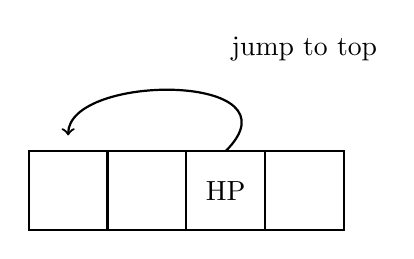
\begin{tikzpicture}
                % Draw the rectangles representing the queue
                \draw[thick] (0,0) rectangle (1,1);
                \draw[thick] (1,0) rectangle (2,1);
                \draw[thick] (2,0) rectangle (3,1);
                \draw[thick] (3,0) rectangle (4,1);
                
                % Arrows to represent "jump to top"
                \draw[->, thick] (2.5, 1) .. controls (3.5, 2) and (0.5, 2) .. (0.5, 1.2);
                
                % Label for high priority
                \node at (2.5, 0.5) {HP};
                
                % Label for "jump to top"
                \node at (3.5, 2.3) {jump to top};
            \end{tikzpicture}
        \end{center}
    \end{definition}
\newpage

\section{Quicksort (Ch. 7, L10)} % DONE except WS (formal) and AC.
\subsection{Key takeaways}
\begin{intuition}
    \begin{itemize}
        \item \textbf{Worst case running time:} $\Theta(n^2)$ (occurs when the list is already sorted)
        \item \textbf{Best case running time:} $\Theta(n \log n)$
        \item \textbf{Averaged/Expected case running time:} $\Theta(n \log n)$
        \item Quicksort tends to have the smallest constant in front of its running time
        \item Quicksort is \textbf{NOT stable} (although there are modified versions that are)
        \item Quicksort is \textbf{in-place} (although this is disputed because it uses recursion, so it stores stuff on the stack, and depends on your exact definition of in-place)
        \item The idea of a randomized algorithm, why randomization helps, and how to analyze a random algorithm
        \item Space complexity is also disputed due to the recursion in Quicksort. It could be $\Theta(1)$ or $O(\log n)$ or $O(n)$ depending on the implementation
    \end{itemize}    
\end{intuition}

\subsection{Intro}
    \subsubsection{QS algorithm}
    \begin{definition}
        \begin{lstlisting}[language=Python, caption={Quicksort Algorithm Pseudocode with Comments}]
            Quicksort (list in, int left, int right):
                pivot = Partition(in, left, right)   # Partition the list and return the pivot 
                if (pivot > left):                  # If elements on the LS of pivot
                    Quicksort(in, left, pivot)      # Apply QS on the left partition
                if (pivot < right):                 # If elements on the RS of pivot
                    Quicksort(in, pivot + 1, right) # Apply QS on the right partition
        \end{lstlisting}
    \end{definition}

    \begin{intuition}
        \begin{itemize}
            \item \textbf{Quicksort is a divide-and-conquer algorithm:}
            \begin{itemize}
                \item The main idea is to partition the list around a \textbf{pivot element}.
                \item After partitioning, the pivot element is placed in its correct position.
            \end{itemize}
            
            \item \textbf{Steps of Quicksort:}
            \begin{itemize}
                \item \textbf{Choose a pivot element:} This can be the first element, the last element, or any random element in the array.
                \item \textbf{Partitioning:} 
                \begin{itemize}
                    \item Elements smaller than the pivot are moved to the left.
                    \item Elements larger than the pivot are moved to the right.
                \end{itemize}
                \item \textbf{Recursively apply Quicksort:}
                \begin{itemize}
                    \item Apply Quicksort to the subarray to the left of the pivot.
                    \item Apply Quicksort to the subarray to the right of the pivot.
                \end{itemize}
            \end{itemize}
            
            \item \textbf{Base case:}
            \begin{itemize}
                \item When the subarray has one or zero elements, it is already sorted, and no further partitioning is needed.
            \end{itemize}
        \end{itemize}        
    \end{intuition}

    \begin{intuition}
        \customFigure[1]{00_Images/Quicksort_Example1.png}{Quicksort example.}          
    \end{intuition}

    \subsubsection{Partition}
    \begin{definition}
        \begin{lstlisting}[language=Python, caption={Partition Function Pseudocode with Comments}]
            int Partition (in, left, right):
                ls = left                        # Left pointer (starting index)
                pivot = in(left)                 # Choose the leftmost element as the pivot
                for i = left + 1 to right:       # Iterate over the rest of the elements
                    if (in(i) <= pivot):         
                        ls = ls + 1              # Increment ls to track smaller elements
                        swap(in(i), in(ls))      # Swap current element with the element at ls
                swap(in(left), in(ls))           # Place pivot element in correct position
                return ls                        # Return the index of the pivot
        \end{lstlisting}


        \customFigure[0.5]{00_Images/QS_LS.png}{Partition}
    \end{definition}

    \begin{intuition}
        \begin{itemize}
            \item The array is separated into 4 parts: $[\text{pivot} \; | \; \leq \text{pivot} \; | \; > \text{pivot} \; | \; \text{unanchored}]$
            \item At each iteration, examine an element in the unanchored part, compare to the pivot, and put it in the appropriate section.
        \end{itemize}
    \end{intuition}

\subsection{QS basic analysis}
    \subsubsection{Best case}
    \begin{derivation}
        The array is always split exactly in half (i.e. picking the median as the pivot), leading to a balanced partition. The recurrence relation for quicksort in this scenario is:

        \begin{equation*}
            T(n) = 2T\left(\frac{n}{2}\right) + \Theta(n)
        \end{equation*}
        \begin{itemize}
            \item $T\left(\frac{n}{2}\right)$: Time to sort $n/2$ elements.
            \item $\Theta(n)$: Time for partition
        \end{itemize}

        \begin{center}
            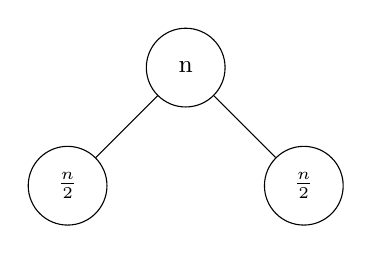
\begin{tikzpicture}[level distance=1.5cm, sibling distance=3cm, every node/.style={circle, draw, minimum size=1cm, font=\small}]
                % Root level for BC
                \node {n}
                    % First level of BC partitioning
                    child {node {$\frac{n}{2}$}}
                    child {node {$\frac{n}{2}$}};
            \end{tikzpicture}
        \end{center}

        \noindent Now using the Master Theorem:
        \begin{equation*}
        T(n) = \Theta(n \log n)
        \end{equation*}
    \end{derivation}

    \subsubsection{Worst case (informal)}
        \begin{derivation}
            The array is already sorted (or reverse sorted) and we choose the first or last element as the pivot, the recurrence relation for quicksort is:

            \[
            T(n) = T(n-1) + \Theta(n)
            \]

            \begin{center}
                % Worst Case (WC) Tree
                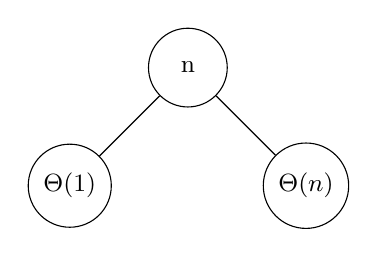
\begin{tikzpicture}[level distance=1.5cm, sibling distance=3cm, every node/.style={circle, draw, minimum size=1cm, font=\small}]
                    % Root level for WC
                    \node {n}
                        % First level of WC partitioning
                        child {node {$\Theta(1)$}}
                        child {node {$\Theta(n)$}};
                \end{tikzpicture}
            \end{center}

            \noindent This recurrence relation expands as follows:

            \begin{align*}
                T(n) &= T(n-1) + \Theta(n) \\
                    &= \left(T(n-2) + \Theta(n-1)\right) + \Theta(n) \\
                    &= \left(T(n-3) + \Theta(n-2)\right) + \Theta(n-1) + \Theta(n) \\
                    &= \cdots \\
                    &= \Theta\left(\sum_{i=1}^{n} i\right) \\
                    &= \Theta\left(\frac{n(n+1)}{2}\right) \\
                    &= \Theta(n^2)
            \end{align*}
            \begin{itemize}
                \item $\Theta(n)$: Time to partition $n$ elements.
                \item $\Theta(n-1)$: Time to partition $n-1$ elements.
                \item $\Theta(n-2)$: Time to partition $n-2$ elements.
                \item $T(n-1)$: Time to sort $n-1$ elements.
            \end{itemize}
        \end{derivation}

    \subsubsection{Expected case}
    \begin{derivation}
        In the average case, the recurrence relation for quicksort can be expressed as:

        \[
        T(n) = T\left(\frac{n}{10}\right) + T\left(\frac{9n}{10}\right) + \Theta(n)
        \]
        \begin{itemize}
            \item \textbf{Key:} Both sides are proportional to $n$.
            \item $T\left(\frac{n}{10}\right)$: Time to sort $n/10$ elements.
            \item $T\left(\frac{9n}{10}\right)$: Time to sort $9n/10$ elements.
            \item $\Theta(n)$: Time to partition $n$ elements.
        \end{itemize}

        \noindent We can visualize this with a recursion tree:

        \customFigure[0.5]{00_Images/Quicksort_Average.png}{Quicksort average case in which each level is derived by subbing in the $T(\#)$ back into the equation above.}          

        \noindent Based on the recursive tree structure and the average-case recurrence relation, we can derive the time complexity as follows:

        \[
        T(n) = h \cdot \Theta(n)
        \]

        \noindent Now, let's calculate the height \( h \) of the tree using the largest element (i.e. right sub-tree):

        \[
        \left(\frac{9}{10}\right)^h n = 1
        \]

        \[
        h = \log_{10/9}(n) 
        \]

        \noindent Substituting this back into the overall complexity:

        \begin{align*}
        T(n) &= h \cdot \Theta(n) \\
            &= \log_{10/9}(n) \cdot \Theta(n) \\
            &= \Theta(n \log n)
        \end{align*}

    \end{derivation}

    \begin{intuition}
        Another way to do the expected case is 
        \begin{center}
            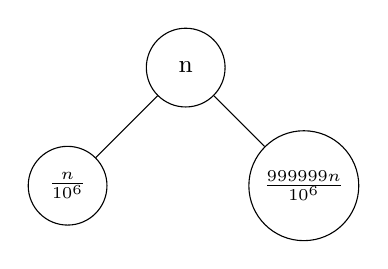
\begin{tikzpicture}[level distance=1.5cm, sibling distance=3cm, every node/.style={circle, draw, minimum size=1cm, font=\small}]
                % Root level
                \node {n}
                    % First level of partitioning
                    child {node {$\frac{n}{10^6}$}}
                    child {node {$\frac{999999n}{10^6}$}};
            \end{tikzpicture}
        \end{center}
        
        \noindent In this example, the array of size \( n \) is split into highly unbalanced sub-arrays:
        \begin{itemize}
            \item One sub-array is \( \frac{n}{10^6} \), very small compared to \( n \).
            \item The other sub-array is \( \frac{999999n}{10^6} \), almost the entire size of \( n \).
        \end{itemize}
        \vspace{1em}

        \textbf{Key:} Both cases represent different ways of dividing the input array in the Quicksort algorithm. Even though the specific subarray sizes differ in each approach, the fundamental property of the algorithm — that it breaks the problem down recursively and performs $\Theta(n)$ work at each level.
    \end{intuition}

\subsection{Worst-case (formal)}
    \begin{derivation}
        The worst-case recurrence relation for quicksort can be expressed as:

        \[
        T(n) = \text{time to QS n-elements} = \max_{1 \leq q \leq n-1} \{ T(q) + T(n-q) \} + \Theta(n)
        \]

        \begin{center}
            % Worst Case (WC) Tree
            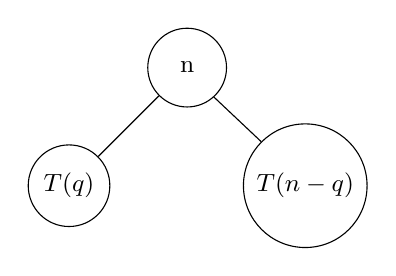
\begin{tikzpicture}[level distance=1.5cm, sibling distance=3cm, every node/.style={circle, draw, minimum size=1cm, font=\small}]
                % Root level for WC
                \node {n}
                    % First level of WC partitioning
                    child {node {$T(q)$}}
                    child {node {$T(n-q)$}};
            \end{tikzpicture}
        \end{center}
        
        \begin{itemize}
            \item $T(n)$: Represents the time to quicksort $n$ elements.
            \item $\max_{1 \leq q \leq n-1}$: Accounts for the worst-case partitioning, where $q$ is the size of one partition and $n-q$ is the size of the other.
            \item $T(q) + T(n - q)$: Represents the time to recursively quicksort the two subarrays of sizes $q$ and $n-q$.
            \item $\Theta(n)$: Represents the linear time required to partition the array around the pivot element.
        \end{itemize}
        \vspace{1em}

        \noindent We use substitution to show that \( T(n) \leq cn^2 \) for some constant \( c \).
        \begin{enumerate}
            \item Guess \( T(n) \leq cn^2 \).
            \item 
        \end{enumerate}
        \begin{align*}
            T(n) &\leq \max_{1 \leq q \leq n-1} \left\{ cq^2 + c(n-q)^2 \right\} + \Theta(n) \quad \text{(Achieves max at } q = 1 \text{ or } q = n-1 \text{ because it's upward quadratic)} \\
                 &= c \max_{1 \leq q \leq n-1} \left\{ q^2 + (n-q)^2 \right\} + \Theta(n) \quad \text{(As second derivative is positive (i.e. monotonic), plug } q = 1 \text{)} \\
                 &\leq cn^2 - 2c(n-1) + \Theta(n) \quad \text{(We can pick a large } c \text{ so that } 2c(n-1) \text{ dominates } \Theta(n)) \\
                 &\leq cn^2
        \end{align*}

        \noindent Therefore, using the substitution method, we can show that \( T(n) \leq cn^2 \), confirming that the worst-case time complexity of the quicksort algorithm is \( O(n^2) \).
    \end{derivation}

\subsection{Expected randomized case (formal)}
    \subsubsection{Motivation for randomized QS}
    \begin{intuition}
        \begin{itemize}
            \item Avoiding worst-case scenarios
            \item Ensuring balanced splits
            \item Works against sorted and reverse sorted arrays.
        \end{itemize}
    \end{intuition}

    \subsubsection{Random partition}
    \begin{definition}
        \begin{lstlisting}[language=Python, caption={Rand-Partition Function Pseudocode}]
            Rand-Partition (list in, left, right)
                i = random(left, right)
                swap(in(left), in(i))
                return Partition(in, left, right)
        \end{lstlisting}
        \begin{itemize}
            \item \textbf{Note:} This partition will be used to find the pivot instead in QS as it will swap random elements.
        \end{itemize}
    \end{definition}

    \subsubsection{Random partition QS}
    \begin{definition}
        \begin{lstlisting}[language=Python, caption={QuickSort with Random Partition}]
            def QS(C):
                pivot = RAND_partition(C)
                
                if pivot > left:
                    QS(C[left : pivot])
                    
                if pivot < left:
                    QS(C[pivot : right])
            \end{lstlisting}            
    \end{definition}

    \begin{derivation}
        \[
        T(n) = \frac{1}{n} \left( T(1) + T(n-1) + \sum_{z=1}^{n-1} T(z) + T(n-z) \right) + \Theta(n)
        \]
        \begin{itemize}
            \item $\frac{1}{n}$: Averages over all possible pivots (i.e. makes it so it's the probability of choosing any element as the pivot)
            \item $T(1) + T(n - 1)$: Represents the time to sort when the pivot results in extreme partitioning, leaving subarrays of size 1 and $n-1$.
            \item $\sum_{z=1}^{n-1} \left(T(z) + T(n - z)\right)$: Represents the sum of the time to sort subarrays formed by all possible partitions where the pivot splits the array into subarrays of size $z$ and $n-z$.
            \item $\Theta(n)$: Represents the linear time required to partition the array around the randomly chosen pivot.
        \end{itemize}
        \vspace{1em}

        To make modifications to the above statement:

        \begin{itemize}
            \item \textbf{Pivot Small:} $\frac{1}{n} (T(1) + T(n-1)) \leq (\Theta(n^2) + \Theta(1)) \cdot \frac{1}{n} \leq \Theta(n)$
            \begin{itemize}
                \item \textbf{Got rid of \( T(1) + T(n-1) \).}
            \end{itemize}
            
            \item \textbf{There are this many elements smaller than the pivot:} $\sum_{z=1}^{n-1} T(z) + T(n-z)$
            
            \item \textbf{Merging:} $\sum_{q=1}^{n-1} \left( T(q) + T(n - q) \right)$ can be simplified to $2 \sum_{k=1}^{n-1} T(k)$ because each subproblem $T(q)$ and $T(n - q)$ is counted twice, effectively merging the two subproblems and leading to a factor of 2.
        \end{itemize}
        \vspace{1em}

        Therefore,
        \[
        T(n) \leq \frac{1}{n} \left[ \sum_{q=1}^{n-1} T(q) + T(n-q) \right] + \Theta(n) = \frac{2}{n} \sum_{k=1}^{n-1} T(k) + \Theta(n)
        \]
        \vspace{1em}

        \textbf{Use substitution to prove \( T(n) = a \log(n) + b \) for proper \( a \), \( b \).}
        \begin{enumerate}
            \item Prove the lemma $\sum_{k=1}^{n-1} k \log(k) \leq \frac{1}{2} n^2 \log(n) - \frac{1}{8} n^2$
            \begin{align*}
                \sum_{k=1}^{n-1} k \log(k) &\leq \sum_{k=1}^{\left\lceil \frac{n}{2} \right\rceil-1} k \log(k) + \sum_{k=\left\lceil \frac{n}{2} \right\rceil}^{n-1} k \log(k) \quad \text{break the summation in half} \\
                &\leq \log \left(\frac{n}{2}\right) \cdot \sum_{k=1}^{\left\lceil \frac{n}{2} \right\rceil-1} k + \log(n) \sum_{k=\left\lceil \frac{n}{2} \right\rceil}^{n-1} k \\
                &= (\log n - \log 2) \cdot \sum_{k=1}^{\left\lceil \frac{n}{2} \right\rceil-1} k + \log(n) \sum_{k=\left\lceil \frac{n}{2} \right\rceil}^{n-1} k \\
                &= \log(n) \sum_{k=1}^{n/2} k - \sum_{k=1}^{n/2} k + \log(n) \sum_{k=n/2}^{n-1} k \\
                &= \log(n) \sum_{k=1}^{n-1} k - \sum_{k=1}^{\frac{n}{2}-1} k \\
                &\leq \frac{1}{2}n(n-1) \log(n) - \frac{1}{2} \left(\frac{n}{2} - 1\right) \cdot \frac{n}{2} \\
                &\leq \frac{1}{2} n^2 \log(n) - \frac{1}{8} n^2
            \end{align*}

            \item Prove using substitution:
            \begin{align*}
                T(n) &\leq \frac{2}{n} \sum_{k=1}^{n-1} a k \log(k) + b + \Theta(n) \\
                    &\leq \frac{2}{n} \left( \frac{1}{2} n^2 \log(n) - \frac{1}{8} n^2 \right) a + b + \Theta(n) \quad \text{(by applying the lemma)} \\
                    &= \frac{a}{n} \left( \frac{1}{2} n^2 \log(n) - \frac{1}{8} n^2 \right) + b + \Theta(n) \\
                    &= a n \log(n) - \frac{a}{4} n + b + \Theta(n) \\
                    &= a n \log(n) + \left( b - \frac{a}{4} n + \Theta(n) \right) \\
                    &\leq a n \log(n) + b \quad \text{(for large \(n\), where lower order terms are negligible)}.
            \end{align*}

        \end{enumerate}
    \end{derivation}



\newpage

\section{Counting sort, Radix sort (Ch. 8)}
\subsection{Lower bound on sorting and counting sort}
    \subsubsection{Lower bound on comparison-based sorting}
    \begin{definition}
        No \textbf{comparison-based} sorting algorithm on \textbf{unrestricted} range (i.e. any numbers) can do better than $\Omega(n\log(n))$.    
    \end{definition}

    \subsubsection{Decision tree}
    \begin{definition}
        Any sorting algorithm can be written as a decision tree. (Goes both ways)
    \end{definition}

    \begin{example}
        \customFigure[0.5]{00_Images/Insertion_Sort.png}{Insertion sort.}
    \end{example}

    \begin{theorem}
        Any decision tree for an n-element sorting algorithm has $h=\Omega (n\log n)$
    \end{theorem}

    \begin{derivation}
        \[
        \log(n!) \approx n \log n - n
        \]
        Using Stirling's approximation:
        \[
        n! \approx \sqrt{2\pi n} \left( \frac{n}{e} \right)^n
        \]
        Taking the logarithm of both sides:
        \[
        \log(n!) = n \log n - n + O(\log n)
        \]
        Therefore, \(\log(n!)\) is asymptotically bounded by:
        \[
        \log(n!) = \Theta(n \log n)
        \]
    \end{derivation}

\subsection{Counting sort}
\begin{definition}
    \begin{lstlisting}[language=Python, caption={Counting Sort Pseudocode}]
        C[i] = 0 for all i in [0...k]
        for j = 1 ... length(A) do  # O(n)
            C[A[j]] = C[A[j]] + 1
        for i = 1 ... k /* prefix sums */ # O(k)
            C[i] = C[i] + C[i-1]
        for j = length(A) ... 1 do # O(n)
            B[C[A[j]]] = A[j]
            C[A[j]] = C[A[j]] - 1 
    \end{lstlisting}
    \begin{itemize}
        \item $A$: array to be sorted. 
        \item \textbf{Sorting range:} Assume numbers in range $[0...k]$.
        \item \textbf{Stable sorting:} Not in-place but stable sorting. 
        \begin{itemize}
            \item \textbf{Stable:} Stable sorting in counting sort ensures that elements with equal values retain their relative order from the original input when sorted.
        \end{itemize}
        \item \textbf{Time complexity:} Time $O(n+k)$ if $O(k) = O(n)$ implies $O(n)$
        \item \textbf{Auxilliary arrays:} $C [0\ldots k]$ and $B [1 \ldots n]$.
    \end{itemize}
\end{definition}

\begin{example}
    \begin{enumerate}
        \item \textbf{Create the Input Array \( A \)}:
            \[
            A = [2, 5, 3, 0, 2, 3, 0, 3]
            \]
        
        The elements of \( A \) are integers within a known range (e.g., \( 0 \) to \( 5 \)).

        
        \item \textbf{Count the Occurrences (Frequency Array) (i.e. 1st loop)}:
        \begin{itemize}
            \item Create an auxiliary array \( C \), where each index represents a possible value in \( A \), and the value at each index in \( C \) represents the number of times that value appears in \( A \).
            \item Initialize \( C \) with zeros:
            \[
            C = [0, 0, 0, 0, 0, 0]
            \]
            \item Count the occurrences of each number in \( A \), updating \( C \):
            \[
            C = [2, 0, 2, 3, 0, 1]
            \]
            This tells us:
            \begin{itemize}
                \item \( 0 \) appears 2 times.
                \item \( 1 \) appears 0 times.
                \item \( 2 \) appears 2 times.
                \item \( 3 \) appears 3 times.
                \item \( 5 \) appears 1 time.
            \end{itemize}
        \end{itemize}
        
        \item \textbf{Modify \( C \) to Store the Cumulative Count (i.e. 2nd loop)}:
        \begin{itemize}
            \item Modify the array \( C \) such that each index contains the sum of the counts for all values less than or equal to that index.
            \item The cumulative count helps to determine the final positions of each element in the sorted array.
            \item After modification, \( C \) becomes:
            \[
            C = [2, 2, 4, 7, 7, 8]
            \]
            This means:
            \begin{itemize}
                \item Values \( \leq 0 \) will be placed before index 2.
                \item Values \( \leq 2 \) will be placed before index 4.
                \item Values \( \leq 3 \) will be placed before index 7.
                \item Values \( \leq 5 \) will be placed before index 8.
            \end{itemize}
        \end{itemize}
        
        \item \textbf{Place the Elements in the Sorted Array \( B \) (i.e. 3rd loop)}:
        \begin{itemize}
            \item Iterate through the elements in \( A \), using the cumulative counts in \( C \) to place each element in the correct position in \( B \).
            \item Decrement the corresponding count in \( C \) for each placement to ensure the stability of sorting.
            \item The sorted array \( B \) is:
            \[
            B = [0, 0, 2, 2, 3, 3, 3, 5]
            \]
            \item \textbf{Example of the third loop:} $B(C(A(8)))=B(C(3))=B(7)=A(8)$, so we place the 8th element in A (e.g. 8) into B(7) (i.e. 7th index)
            \vspace{1em}

            $B(C(A(7)))=B(C(0))=B(2)=A(7)$, so we place the 7th element in A (e.g. 0) into B(2) (i.e. 2nd index), 
        \end{itemize}
    \end{enumerate}
    \customFigure[0.5]{00_Images/Counting_Sort.png}{Example of counting sort}
\end{example}

\subsection{Radix sort}
\begin{definition}
    \begin{lstlisting}[language=Python, caption={Radix Sort Pseudocode}]
        for i = Least significant bit (LSB) -> Most significant bit (MSB)
            counting_sort(digit) # or any stable sorting algorithm on digit i
    \end{lstlisting}
\end{definition}

\begin{example}
    The numbers in the image are sorted digit by digit, starting with the least significant digit. 

    \begin{enumerate}
        \item \textbf{Sort by the Least Significant Digit (LSD)}:
        \begin{itemize}
            \item Start by examining the rightmost digit (the units place) of each number.
            \item In the image, the numbers:
            \[
            [512, 413, 242, 375, 695, 112]
            \]
            are sorted by their least significant digits:
            \begin{align*}
            512 & \rightarrow 2, \\
            413 & \rightarrow 3, \\
            242 & \rightarrow 2, \\
            375 & \rightarrow 5, \\
            695 & \rightarrow 5, \\
            112 & \rightarrow 2.
            \end{align*}
            Sorting by the rightmost digits results in:
            \[
            [512, 242, 112, 413, 375, 695]
            \]
        \end{itemize}
        
        \item \textbf{Sort by the Next Significant Digit (Tens place)}:
        \begin{itemize}
            \item After sorting by the least significant digit, now sort the numbers based on the second digit (the tens place).
            \item The current sequence of numbers:
            \[
            [512, 242, 112, 413, 375, 695]
            \]
            is sorted by the tens digit:
            \begin{align*}
            512 & \rightarrow 1, \\
            242 & \rightarrow 4, \\
            112 & \rightarrow 1, \\
            413 & \rightarrow 1, \\
            375 & \rightarrow 7, \\
            695 & \rightarrow 9.
            \end{align*}
            Sorting by the tens place results in:
            \[
            [512, 112, 413, 242, 375, 695]
            \]
        \end{itemize}
        
        \item \textbf{Sort by the Most Significant Digit (Hundreds place)}:
        \begin{itemize}
            \item Finally, sort by the hundreds digit. The current sequence:
            \[
            [512, 112, 413, 242, 375, 695]
            \]
            is sorted by the hundreds digit:
            \begin{align*}
            512 & \rightarrow 5, \\
            112 & \rightarrow 1, \\
            413 & \rightarrow 4, \\
            242 & \rightarrow 2, \\
            375 & \rightarrow 3, \\
            695 & \rightarrow 6.
            \end{align*}
            Sorting by the hundreds place results in the final sorted sequence:
            \[
            [112, 242, 375, 413, 512, 695]
            \]
        \end{itemize}
        
    \end{enumerate}

    \customFigure[0.5]{00_Images/Radix_Sort.png}{Radix sort example}
\end{example}

\subsubsection{Runtime complexity analysis of Radix sort}
\begin{definition}
    \begin{itemize}
        \item \textbf{Variables:}
        \begin{itemize}
            \item n: \# numbers 
            \item r: range of numbers 
            \item d: \# digits
        \end{itemize}

        \item \textbf{One pass complexity:} $=O(n+r)$ (i.e. the time complexity of counting sort)
        \item \textbf{All passes complexity:} $dO(n+r) = O(dn + dr)$ (i.e. sorting all digits, so it's the time complexity of counting sort times the number of digits)
        \item \textbf{r=d complexity:} If $r=d=O(1)$, then $O(n)$ true for all passes.
    \end{itemize}
\end{definition}

\subsubsection{Example of QS vs. RS}
\begin{example}
    Sorting $1000\#$'s, each represented using 64 bits. Each digit is 16 bits wide. 
    \begin{itemize}
        \item \textbf{Quicksort:} $O(n \log(n)) = \frac{O(1000 \log(1000))}{1000}$ (i.e. divided by 1000 to show the average time compared to Radix sort)
        \begin{itemize}
            \item $\log(1000) \approx 10$ passes./number
        \end{itemize} 
        \item \textbf{Radix sort:} $4 \text{ passes/number}$ (i.e. one for each digit)
    \end{itemize}
    \customFigure[0.5]{00_Images/Bits.png}{Number of passes for 1000\#'s 64 bits.}
\end{example}

\subsection{Tournament tree selection}
    \subsubsection{What is the kth largest element in unsorted sequence}
    \begin{definition}
        How many comparisons to find max element? $(n-1)$ 
        \begin{itemize}
            \item \textbf{Max Comparisons:} $n-1$: It's the winner (i.e. root) of the tournament tree. Don't need to check the $nth$ element because it is the biggest.
            \begin{itemize}
                \item \textbf{Note:} Don't need to check the $nth$ element because it is the biggest.
            \end{itemize}
            \item \textbf{Min Comparisons:} $n/2 - 1$: Take the losers (i.e. leaves) of the tournament to find the minimum (assume that we found the maximum already). Since $n/2$ only contains the leaves and we know that the last loser will be the minimum, therefore, $n/2 - 1$ comparisons.
            \item \textbf{2nd Max Comparisons:} $\log n - 1$ additional comparisons after finding the maximum by comparing the max elements battles with other elements (i.e. 2nd biggest loses to max so follow max route). Since the height of the tree is $\log(n)$ and we know the max already, therefore, $\log(n) - 1$
            \item \textbf{Kth Max comparisons:} Total comparisons is the $O((n-1) + k\log n)=O(n+k\log(n))$
            \begin{itemize}
                \item $O(n-1)$: Cost of building the tournament tree by comapring all elements. 
                \item $O(k\log(n))$: Additional comparisons required to identify subsequent maximums. At each level, there are $\log(n)$ comparisons.
            \end{itemize}
        \end{itemize}
        \customFigure[0.5]{00_Images/TT.png}{Tournament tree.}
    \end{definition}

    \subsubsection{Selecting the kth element in O(n) expected time}
    \begin{example}
        How to find the $kth$ element without sorting the array for finding a certain element. For finding a specific element, it is $O(n)$ expected time. Quickselect is a variant of Quicksort used to find the
        k-th smallest or largest element without fully sorting the array.            
        \begin{enumerate}
            \item \textbf{Initial Array:} The original unsorted array is:
            \[
            [8, 1, 5, 9, 2, 10, 4, 17, 20]
            \]
            We are tasked with finding the 7th smallest element when the array is sorted.
            
            \item \textbf{Choosing a Pivot:} In the Quickselect algorithm, the first pivot element chosen is `8`.
            
            \item \textbf{Partitioning Around Pivot:} The array is partitioned into two parts:
            \begin{itemize}
                \item Elements smaller than or equal to `8` are moved to the left.
                \item Elements greater than `8` are moved to the right.
            \end{itemize}
            After partitioning, the array becomes:
            \[
            [1, 5, 2, 4, 8, 9, 10, 17, 20]
            \]
            The pivot `8` is in its correct sorted position (5th position in the array).
            
            \item \textbf{Comparing Pivot Position with Target:} Since we are looking for the 7th smallest element, and `8` is in the 5th position, the desired element must be in the subarray to the right of `8`:
            \[
            [9, 10, 17, 20]
            \]
            Now we search for the 2nd smallest element in this subarray because it corresponds to the 7th smallest element in the overall array.
            
            \item \textbf{Recursive Partitioning:} Another pivot is chosen from the remaining subarray, let’s assume it’s `9`. After partitioning:
            \[
            [9, 10, 17, 20]
            \]
            The pivot `9` is in the 1st position of this subarray (6th position in the overall array).
            
            \item \textbf{Final Step:} Now, we are looking for the 1st smallest element in the subarray:
            \[
            [10, 17, 20]
            \]
            After partitioning, the smallest element is `10`, which is the 7th smallest element in the entire array.
        \end{enumerate}        
    \end{example}

    \subsubsection{Randomized Select (SEE IF HE COVERS THIS IN CLASS)}
    \begin{definition}
        \begin{lstlisting}[language=Python, caption={Randomized Select Algorithm}]
            Randomized_select(A, p, r, i^th):
                if p == r then
                    return A[p]
                
                q = rand_part(A, p, r)
                k = q - p + 1
                
                if i <= k then
                    rand_select(A, p, q, i)
                else
                    rand_select(A, q + 1, r, i - k)
            \end{lstlisting}

        \begin{itemize}
            \item \textbf{Purpose}: The algorithm aims to find the i-th smallest element in an array.
            
            \item \textbf{Steps}:
            \begin{itemize}
                \item \textbf{Base Case}: If the array has only one element (i.e., \( p = r \)), return that element as it is the i-th smallest.
                \item \textbf{Partitioning}: Select a random pivot and partition the array around this pivot (similar to QuickSort). Now, the pivot's position in the sorted array is known.
                \item \textbf{Position Comparison}:
                \begin{itemize}
                    \item If the pivot's position is the i-th smallest, return it.
                    \item If \( i \leq k \) (where \( k \) is the position of the pivot), search the left subarray.
                    \item Otherwise, search the right subarray, adjusting \( i \) to account for the elements eliminated.
                \end{itemize}
            \end{itemize}
        \end{itemize}
        \vspace{1em}

        \begin{equation*}
        T(n) = \frac{1}{n} \left( T(\max(1, n-1)) + \sum_{k=1}^{n-1} T(\max(k, n-k)) \right) + \Theta(n) = O(n)
        \end{equation*}

        \begin{itemize}
            \item \( \frac{1}{n} \): Reflects the randomness of pivot selection over \( n \) possible pivots.
            \item \( T(\max(1, n-1)) \): The best case where the pivot splits the array as unevenly as possible.
            \item \( \sum_{k=1}^{n-1} T(\max(k, n-k)) \): Covers all possible partition sizes and recursive subproblem sizes.
            \item \( \Theta(n) \): Accounts for the partitioning step, which is linear.
        \end{itemize}
    \end{definition}
\newpage

% 4 LECTURES ^

\section{Selection sort, Binary search trees (Ch. 12)}
\subsection{Selection sort}

\subsection{Binary search trees}
\newpage

\section{Red black trees (Ch. 13)}
\subsection{Properties}
\begin{definition}
    Structurally balanced, i.e., \( h = O(\log n) \). RBT is a BST with the following properties:
    \begin{itemize}
        \item Every node is either red or black.
        \item The root is always black.
        \item A red node has black children.
        \item Every path from root to leaf has the same number of black nodes.
    \end{itemize}
\end{definition}

\subsubsection{Black height}
\begin{definition}
    The black height \( bh(x) \) is the number of black nodes on any path to a leaf, excluding \( x \).
    \customFigure[0.5]{00_Images/RBT.png}{Red black trees.}
\end{definition}

\begin{theorem}
    A Red-Black Tree with \( n \) internal nodes has 
    \begin{equation}
        h \leq 2 \log(n+1) = O(\log n)
    \end{equation}
\end{theorem}

\begin{theorem}
    \textbf{Lemma:} A subtree in a Red-Black Tree rooted at \( x \) has at least 
    \begin{equation}
        2^{bh(x)} - 1
    \end{equation}
    internal nodes.
\end{theorem}

\begin{derivation}
    Use induction on \( h \) to prove the theorem

    \begin{enumerate}
        \item  \textbf{Basis:} \( h = 0 \). Only one node, which is black, and \( bh(\text{node}) = 0 \), so we have 0 internal nodes:
        \[
        2^0 - 1 = 0 
        \]
    
        \item \textbf{Hypothesis:} Assume the lemma holds for all heights \( \leq h-1 \).
        
        \item \textbf{Step:} Suppose \( x \) is a red node. Then 
            \[
            bh(x) = bh(x.\text{child}) - 1
            \]
            If \( x \) is black, then
            \[
            bh(x) = bh(x.\text{child})
            \]
            Thus, \( x \) has internal nodes from both children.
            \vspace{1em}
            
            At least how many internal nodes does \( x \) have?
        
            \[
            \begin{aligned}
                & (2^{bh(x)-1} - 1) \quad \text{from the left subtree}, \\
                & (2^{bh(x)-1} - 1) \quad \text{from the right subtree}, \\
                & + 2 \quad \text{for the root and two children}.
            \end{aligned}
            \]
        
            Thus,
            \[
            2(2^{bh(x)-1}) - 1 = 2^{bh(x)} - 1 \quad \checkmark
            \]
        
        \item \textbf{Return to the theorem:}
            \[
            n \geq 2^{bh(\text{root})} - 1 \quad \text{(by the lemma)}.
            \]
        
            Thus,
            \[
            h \leq 2 \log(n+1) = O(\log n)
            \]
    \end{enumerate}
\end{derivation}

\subsection{Balance proof}

\subsection{Operations}
\newpage

% 3 LECTURES ^ 

\section{Hash tables, Hashing (Ch. 11)}
\subsection{Motivation}

\subsection{Resolution by chaining}

\subsection{Resolution by open addressing}
\newpage

% 1 LECTURE ^

\section{Dynamic programming (Ch. 14)}
\subsection{Intro to dynamic programming}
\begin{definition}
    Dynamic programming is an epitome of the "divide and conquer" approach. It often deals with max/min problems, utilizing two key characteristics:
    \begin{enumerate}
        \item \textbf{Optimal substructure:} Break problem into smaller problems of same nature, find solutions to subproblems and combine results 
        \item \textbf{Overlapping subproblems:} The same subproblems are solved multiple times, which can be avoided using \textit{memoization} to store/retrieve the intermediate results.
    \end{enumerate}
\end{definition}

\begin{example}
    Motivation for memoization:
    \begin{equation*}
        f_0 = 0, \quad f_1 = 1, \quad f_i = f_{i-1} + f_{i-2}
        \end{equation*}
        
        For example, consider calculating \(F(100)\):
        
        \customFigure[0.5]{00_Images/S.png}{Fib numbers}
        
        \begin{itemize}
            \item \textbf{Solution:} Notice that during the calculation of \(F(99)\) and \(F(98)\), \(F(98)\) is calculated more than once. Hence, it is efficient to store the computed values in an array and access them directly instead of recalculating (i.e. memoization).
        \end{itemize}
\end{example}

\subsection{DP matrix multiplication}
\subsubsection{Optimal Matrix Parenthesization Problem Setup}
\begin{definition}
    Given matrices \(A_1, A_2, \dots, A_n\), we seek the optimal way to multiply them in that order that minimizes the number of scalar multiplications. 
\end{definition}

\begin{intuition}
Matrix multiplication is associative, but the order in which matrices are multiplied affects the number of operations. The goal is to find the optimal parenthesization that minimizes this count.
\end{intuition}

\begin{example}
    Consider the matrices
    \[
    A_1 \in \mathbb{R}^{10 \times 100}, \quad A_2 \in \mathbb{R}^{100 \times 5}, \quad A_3 \in \mathbb{R}^{5 \times 50}
    \]
    We need to find the minimum cost of multiplying \(A_1 A_2 A_3\).
    \vspace{1em}

    Possible parenthesizations and their associated costs:
    \[
    (A_1 A_2) A_3 = (10 \times 100 \times 5) + (10 \times 5 \times 50) = 7500
    \]
    \begin{itemize}
        \item \textbf{First Term:} $A_1 A_2$: $10 \times 100 \times 5$
        \item \textbf{Second Term:} $(A_1 A_2) \in \mathbb{R}^{10 \times 5}$, so $(A_1 A_2) A_3$: $10 \times 5 \times 50$.
    \end{itemize}
    \vspace{1em}

    \[
    A_1 (A_2 A_3) = (100 \times 5 \times 50) + (10 \times 100 \times 50) = 75000
    \]
    \begin{itemize}
        \item \textbf{First Term:} $A_2 A_3$: $ 100 \times 5 \times 50$
        \item \textbf{Second Term:} $(A_2 A_3) \in \mathbb{R}^{100 \times 500}$, so $(A_1 A_2) A_3$: $100 \times 500 \times 50$
    \end{itemize}
    Thus, the optimal solution is to compute \((A_1 A_2) A_3\) with a cost of 7500 scalar multiplications.
\end{example}

\subsubsection{Total number of parenthesization}
\begin{definition}
    The total number of possible parenthesizations for multiplying \(A_1, A_2, \dots, A_n\):

    \begin{equation*}
    \text{Total number of parenthesizations} = \sum_{k=1}^{n-1} P(k)P(n-k) = \Omega \left(\frac{4^n}{n^{3/2}}\right) 
    \end{equation*}
    \begin{itemize}
        \item \textbf{Note:} The solution is given since we don't know hwo to solve the reccurrence. 
        \item \textbf{Key:} Therefore the brute force method of calculating all the parenthesizations and finding the minimum amount is non-trivial due to when $n\rightarrow \infty$.
    \end{itemize}
   
\end{definition}

\subsubsection{Recursive Formula for Cost}
\begin{definition}
    Let matrix \(A_i = P_{i-1} \times P_i\) denote the dimensions of the matrix, and let \(A_{ij} = A_i \cdots A_j\) represent the product of matrices from \(i\) to \(j\).
    \vspace{1em}

    The recursive formula for the minimal cost \(m(i,j)\) (i.e. optimal number of SM to evaluate matrices \(A_i \dots A_j\)) is given by:

    \begin{equation*}
    m(i,j) = 
    \begin{cases}
    0 & \text{if} \quad i = j \\
    \min_{i \leq k < j} \left( m[i,k] + m[k+1,j] + P_{i-1} P_k P_j \right) & \text{if} \quad i < j
    \end{cases}
    \end{equation*}
    \begin{itemize}
        \item \textbf{Purpose:} Find the optimal substructure (i.e. first principle of dynamic programming)
        \item \textbf{Intuition:} Find which $k$ minimizes the SM of the matrices on the left of $k$ and the right of $k$, which is $m[i,k]$ (left) $m[k+1,j]$ (right). The final term \(P_{i-1} P_k P_j\) comes from multiplying $m[i,k]$, and $m[k+1,j]$ together. 
        \begin{itemize}
            \item $A_1 A_2 \cdots A_i \cdots A_k A_{k+1} \cdots A_j \cdots A_{n-1} A_n$
            \begin{itemize}
            \item $A_i \cdots A_k = A_{ik}$ and $A_{k+1} \cdots A_j = A_{(k+1)j}$
            \end{itemize}
        \end{itemize} 
    \end{itemize}
\end{definition}

\subsubsection{Why is the first principle (i.e. optimal substructure) not sufficient?}
\begin{example}

    \customFigure[0.75]{00_Images/EX1.png}{Why memoization is needed}

    \begin{itemize}
        \item \textbf{Note:} This recursive pattern is similar to the approach used for Fibonacci sequence calculations, highlighting overlapping subproblems. So memoization is needed.
        \begin{itemize}
            \item \textbf{Store:} Store the results in a 2D array since we have two different indices $i$ and $j$.
        \end{itemize}
    \end{itemize}
\end{example}

\subsubsection{Matrix Chain Multiplication Example}
\begin{example}
    Consider the matrices with the following dimensions:

    \[
    A_1: 30 \times 35, \quad A_2: 35 \times 15, \quad A_3: 15 \times 5, \quad A_4: 5 \times 10, \quad A_5: 10 \times 20, \quad A_6: 20 \times 25
    \]

    The goal is to find the minimum cost of multiplying these matrices together and store them in a 2D result.
    \vspace{1em}

    The triangle below represents the minimum number of scalar multiplications needed for each subproblem. Each entry in the triangle corresponds to the cost of multiplying the matrices from \(A_i\) to \(A_j\). 

    \customFigure[0.5]{00_Images/M.png}{You do not need the whole 2D array, you just need the upper triangle of the 2D array. Calculate this table from the bottom up.}
    \begin{itemize}
        \item \textbf{Key:} $\text{cell}(i,j)$ holds $m(i,j)$.
        \item \textbf{Bottom Row:} All zeros because there is no scalar multiplication when $i=j$ (i.e. same matrix)
        \item \textbf{1-2}: $30 \times 35 \times 15$
        \item \textbf{1-3} $A_1 A_2 A_3$ either with $(A_1 A_2)A_3$ and $A_1 (A_2A_3)$
        \begin{itemize}
            \item $(A_1 A_2)A_3$: $15750 + 30 \times 15 \times 5$
            \item $A_1 (A_2A_3)$: $2625 + 30 \times 35 \times 5$ (this one is smaller), so $m(1,3)$ is this. 
            \begin{itemize}
                \item \textbf{Note:} Use an arrow to denote from which bottom row is made.  
            \end{itemize}
        \end{itemize}
        \item \textbf{1-4}: We will now calculate the cost for multiplying a subset of the matrices $A_1 A_2 A_3 A_4$.
        \begin{enumerate}
            \item First, consider multiplying \(A_1[A_2 A_3 A_4]\):
            \[
            = 4375 + (30 \times 35 \times 10) = 4375 + 10500 = 14875
            \]
            \item Now, consider multiplying \([A_1 A_2][A_3 A_4]\):
            \[
            = 15750 + 750 + (30 \times 15 \times 10) = 15750 + 750 + 4500 = 21000
            \]
        
            \item Finally, consider multiplying \([A_1 A_2 A_3] A_4\):
            \[
            = 7875 + (30 \times 5 \times 10) = 7875 + 1500 = 9375
            \]
        \end{enumerate}
        \begin{itemize}
            \item \textbf{Note:} This is made easier using memoization.
        \end{itemize}
        Thus, the optimal solution $m(1,4)$ for multiplying \(A_1 A_2 A_3 A_4\) is \(9375\) scalar multiplications.
    \end{itemize}
    \vspace{1em}
\end{example}

\subsubsection{Time Complexity}
\begin{definition}
    The time complexity of this algorithm is determined by the number of subproblems (or squares in the table), leading to a total complexity of:

    \[
    n \mathcal{O}(n^2) = \mathcal{O}(n^3)
    \]
    \begin{itemize}
        \item \textbf{Note:} where \(n\) is the index since the index can go up to $n$ times for $m(i,j)$ since we have to find the lowest one. 
    \end{itemize}
\end{definition}

\subsection{DP longest common subsequence (LCS)}
\begin{definition}
Given two strings \(X = x_1, x_2, \dots, x_m\) and \(Y = y_1, y_2, \dots, y_n\), the longest common subsequence (LCS) of \(X\) and \(Y\) is the longest sequence that appears in both strings in the same order, though not necessarily consecutively.
\begin{itemize}
    \item \textbf{Notation:} Let \(X^k = x_1, x_2, \dots, x_k\) denote a substring of \(X\) (lower case are characters and upper case is a string)
\end{itemize}
\end{definition}

\begin{example}
    \begin{itemize}
        \item Suppose we are given two strings, "springtime" and "pioneer". 
        \item pine is the LCS (i.e. $LCS=4$).
    \end{itemize}
\end{example}

\subsubsection{Naive Approach / Brute Force Approach}
\begin{intuition}
    Assuming \(m \leq n\), a brute force solution has a time complexity of \(\Theta(n 2^m)\) ("matching each char. of X with Y")
    \begin{itemize}
        \item Have to generate all possible combinations of one string, which is $2^m$ since $m$ is the smaller integer. We can either include or exclude a character from the subsequence, which is the reason for base $2$.
        \item Have to make each subsequence with the other string, requiring $n$ for each. 
    \end{itemize}
\end{intuition}

\subsubsection{Theorem}
\begin{theorem}
If \(Z = z_1, z_2, \dots, z_k\) is the LCS of \(X\) and \(Y\), then:
\begin{itemize}
    \item[(A)] If \(x_m = y_n\), then \(x_m = y_n = z_k\) and \(z_{k-1}\) is the LCS of \(X_{m-1}\) and \(Y_{n-1}\).
    \item[(B)] If \(x_m \neq y_n\), then \(z_k \neq x_m\), so \(Z\) is the LCS of \(X_{m-1}\) and \(Y_n\).
    \item[(C)] If \(x_m \neq y_n\), then \(z_k \neq y_n\), so \(Z\) is the LCS of \(X_m\) and \(Y_{n-1}\).
\end{itemize}
\end{theorem}

\begin{intuition}
    \begin{enumerate}
        \item \textbf{(A)} If $x_m = y_n$, then $x_m = y_n = z_k$ and $z_{k-1}$ is the LCS of $X_{m-1}$ and $Y_{n-1}$.
        
        \textbf{Example:} Let $X = \text{"ABC"}$ and $Y = \text{"ADC"}$. The LCS is $Z = \text{"AC"}$.
        \begin{itemize}
            \item Here, $x_3 = C$ and $y_3 = C$, so $x_3 = y_3 = z_2 = C$.
            \item The LCS of $X_2 = \text{"AB"}$ and $Y_2 = \text{"AD"}$ is $z_1 = A$, which satisfies part (A).
        \end{itemize}
        
        \item \textbf{(B)} If $x_m \neq y_n$, then $z_k \neq x_m$, so $Z$ is the LCS of $X_{m-1}$ and $Y_n$.
        
        \textbf{Example:} Let $X = \text{"ABC"}$ and $Y = \text{"ABDF"}$. The LCS is $Z = \text{"AB"}$.
        \begin{itemize}
            \item Here, $x_3 = C$ and $y_4 = F$, so $x_3 \neq y_4$.
            \item Since $z_2 = B \neq x_3 = C$, the LCS of $X_2 = \text{"AB"}$ and $Y_4 = \text{"ABDF"}$ is still $Z = \text{"AB"}$, which satisfies part (B).
        \end{itemize}
        
        \item \textbf{(C)} If $x_m \neq y_n$, then $z_k \neq y_n$, so $Z$ is the LCS of $X_m$ and $Y_{n-1}$.
        
        \textbf{Example:} Let $X = \text{"ABC"}$ and $Y = \text{"BACD"}$. The LCS is $Z = \text{"AC"}$.
        \begin{itemize}
            \item Here, $x_3 = C$ and $y_4 = D$, so $x_3 \neq y_4$.
            \item Since $z_2 = C \neq y_4 = D$, the LCS of $X_3 = \text{"ABC"}$ and $Y_3 = \text{"BAC"}$ is still $Z = \text{"AC"}$, which satisfies part (C).
        \end{itemize}
    \end{enumerate}
\end{intuition}

\begin{derivation}
    \textbf{Proof of (A):}
    \begin{enumerate}
        \item ATaC that \(x_m = y_n = z_k\), but \(Z_{k-1}\) is not the LCS of \(X_{m-1}\) and \(Y_{n-1}\). 
        \item As a result, some other string \(W\) would be the LCS, so $|W|>|Z_{k-1}|$
        \item This implies \(|W| \cup z_k > |Z_{k-1}| \cup z_k = Z\) (i.e. appending the last character). However, this contradicts the assumption that \(Z\) is the longest common subsequence in the theorem
        \begin{itemize}
            \item \textbf{Note:} When you append $z_k$ to $|Z_{k-1}|$, you are forming $Z$.
        \end{itemize}
    \end{enumerate}
    \begin{itemize}
        \item (B) and (C) follow similarly by considering the cases where \(x_m \neq y_n\).
    \end{itemize}
\end{derivation}

\begin{intuition}
If the last characters of \(X\) and \(Y\) match, they are part of the LCS. Otherwise, we reduce the problem by eliminating the last character of either \(X\) or \(Y\) and finding the LCS of the reduced strings.
\end{intuition}

\subsubsection{Dynamic Programming Approach}
\begin{definition}
    \(C[i, j]\) is the length of the LCS of \(X_i\) and \(Y_j\) (i.e. number of characters of the LCS)

    \begin{equation}
    C[i, j] = 
    \begin{cases}
    0 & \text{if} \quad i = 0 \quad \text{or} \quad j = 0 \\
    C[i-1, j-1] + 1 & \text{if} \quad x_i = y_j \quad \text{(case A)} \\
    \max(C[i-1, j], C[i, j-1]) & \text{if} \quad x_i \neq y_j \quad \text{(cases B, C)}
    \end{cases}
    \end{equation}

\end{definition}

\begin{intuition}
    \begin{itemize}
        \item \textbf{Base Case: \(i = 0\) or \(j = 0\)}\\
        \textit{Explanation:} When either string is of length zero, the LCS is also zero since no common subsequence can exist.\\
        \textit{Example:} If \(X = "ABC"\) and \(Y = ""\), then the LCS length is 0 because one of the strings is empty.
    
        \item \textbf{Case A: \(x_i = y_j\)}\\
        \textit{Explanation:} If the characters at position \(i\) in \(X\) and \(j\) in \(Y\) match, we extend the current LCS by 1 because we have found a common character.\\
        \textit{Example:} Let \(X = "ABC"\) and \(Y = "ADC"\). If we are at \(i = 3\) and \(j = 3\) (comparing \(X_3 = C\) and \(Y_3 = C\)), since they match, the value of \(C[3,3] = C[2,2] + 1\), extending the LCS length by 1.
    
        \item \textbf{Case B and C: \(x_i \neq y_j\)}\\
        \textit{Explanation:} If the characters at position \(i\) and \(j\) do not match, the LCS could either:
        \begin{itemize}
            \item Exclude the current character from \(X\), and look at \(C[i-1,j]\).
            \item Exclude the current character from \(Y\), and look at \(C[i,j-1]\).
        \end{itemize}
        \textit{Intuition:} We take the maximum of these two possibilities because we want the longest subsequence.\\
        \textit{Example:} Let \(X = "ABC"\) and \(Y = "ABD"\). If we are at \(i = 3\) and \(j = 3\) (comparing \(X_3 = C\) and \(Y_3 = D\)), they don’t match, so we take \(C[2,3]\) or \(C[3,2]\), whichever is larger.
    \end{itemize}    
\end{intuition}

\subsubsection{Memoization}
\begin{example}
    Given bojo $4$ and bat $3$, then 
    \begin{example}
        \customFigure[0.75]{00_Images/BOJI.png}{Motivation for why memoization is needed.}
    \end{example}
    \begin{itemize}
        \item \textbf{Memoization:} Store results in a 2D array since we have two indices running.
    \end{itemize}
\end{example}

\begin{definition}
    Another representation is the 2 by 2. 
    \customFigure[0.75]{00_Images/2b2.png}{2 by 2 matrix.}
    \begin{itemize}
        \item Representation of the 3 cases: 

        \begin{itemize}
            \item \textbf{Base Case:} $C[i,j] = 0$ when either string is empty. This initializes the matrix where the LCS length starts at zero.
            
            \item \textbf{Case A:} If $x_i = y_j$, $C[i,j] = C[i-1, j-1] + 1$. This corresponds to part (A) of the theorem, where matching characters extend the LCS. The diagonal arrow in the diagram reflects this, indicating that the LCS grows by $+1$.
            
            \item \textbf{Cases B and C:} If $x_i \neq y_j$, $C[i,j] = \max(C[i-1, j], C[i, j-1])$. This matches parts (B) and (C) of the theorem, where non-matching characters lead to taking the maximum LCS by either excluding $x_i$ or $y_j$. The horizontal and vertical arrows in the diagram represent this decision.
        \end{itemize}

    \end{itemize}
\end{definition}

\begin{example}
Consider the strings \(X = \text{spanking}\) and \(Y = \text{amputation}\). The dynamic programming table for \(C[i,j]\) is shown below.

\customFigure[0.5]{00_Images/LCS1.png}{Computation of C}
\begin{itemize}
    \item \textbf{Base case:} Since the top left has no characters, we fill up the first column and row with zeros. 
    \item \textbf{Algorithm procedure:} 
    \begin{enumerate}
        \item Go column by column or row by row. 
        \item Compare the letters and the arrows represent the previous subproblem being added to the the previous subproblem. This relates to the 2by2 matrix. 
        \begin{itemize}
            \item Take the maximum when the characters are not the same, and go diagonally when they are the same character.
            \item \textbf{Note:} We are only focused on one pathway for this that gives the maximum length of the LCS. 
        \end{itemize}
        \item C gives you the length, but you don't know the actual LCS, but you the length of the LCS is $4$ (i.e. number of diagonals). 
        \item So whenever you have a diagonal you circle the letter, so you get the word pain as the LCS.
    \end{enumerate}
\end{itemize}

\end{example}

\subsubsection{Time Complexity}
\begin{definition}
    The time complexity of this approach is 
    \begin{equation}
        \mathcal{O}(m \times n)
    \end{equation}
    \begin{itemize}
        \item \(m\) is the length of string \(X\)
        \item \(n\) is the length of string \(Y\). 
        \item \textbf{Note:} The algorithm fills a table of size \(m \times n\), and for each cell, it performs a constant number of operations.
    \end{itemize}
\end{definition}
\newpage

% 2 LECTURES ^ 

\section{Greedy algorithms (Ch. 15)} % MIDTERM CUT
\subsection{Greedy Algorithms Intro and Class Scheduling}

\begin{intuition}
    \begin{itemize}
        \item "Greed works, greed is right, greed is good." 
        \item Greedy algorithms make locally optimal choices at each stage with the goal of finding a global optimum. This approach can approximate NP-complete problems.
    \end{itemize}
\end{intuition}

\subsubsection{Characteristics}
\begin{definition}
        Greedy algorithms are good for max/min problems. 
        \begin{itemize}
            \item \textbf{Optimal substructure:} Same as DP
            \item \textbf{Greedy principle:} At every step do greedy choice that looks at the best option at the time begin (i.e. aims to identify and select the most favorable choice at each of the given stagesaims to identify and select the most favorable choice at each of the given stages). 
        \end{itemize}
\end{definition}

\begin{warning}
    You will need to do a proof of correctness for DP and GA.
\end{warning}

\subsubsection{Class Scheduling Example}
\begin{example}
    Given one room and many classes to schedule, the goal is to maximize the number of classes scheduled in one day. The greedy aprooach is that
    \begin{enumerate}
        \item Sort by finish time (i.e. start with the class that starts more early)
        \item Schedule classes in order based on sorted times.
        \item The time complexity for sorting is $O(n\log(n))$.
    \end{enumerate}
    \customFigure[0.75]{00_Images/CSE.png}{Class scheduling example.}

\end{example}

\subsubsection{Proof of Correctness of Class Scheduling (On exams)}
\begin{derivation}

    Prove $g_1,\ldots,g_m$ is optimal:
    \begin{itemize}
        \item ATaC: Given that greedy choices $g_1, g_2, \dots, g_m$ are not optimal, but some other optimal choices $o_1, o_2, \dots, o_m$ exist $(m > n)$. 
        \item By the way the greedy algorithm works, $f(g_i) \leq f(o_i)$ (f is the finish time) because it replaces based on the finish time. 
        \customFigure[0.75]{00_Images/POC.png}{WHAT IS THIS EXAMPLE SHOWING.}
        \begin{itemize}
            \item You can replace $o_1$ with $g_1$ by construction because $g_1$ finishes first. 
            \item You can replace $o_2$ with $g_2$ by constrcution 
            \item Up to $g_m$
            \item $o_{m+1} \ldots o_k$ cannot exist because the greedy algorithm didn't pick any. So we proved that the optimal solution is $G$
        \end{itemize}
        \item $o_{n+1},\dots, o_m$ cannot exist as greedy algorithm would take these into account, therefore, this implies a contradiction since the greedy algorithm would take these into account.
        \item Therefore, $O=G$ and $G=\text{optimal}$.
    \end{itemize}
\end{derivation}

\begin{warning}
    Usually use proof by contradiction. 
\end{warning}

\subsection{Knapsack Problem (Show Difference B/W DP and GA)}

\subsubsection{Problem setup}
\begin{intuition}
A thief breaks into a store and the thief's bag can carry up to $\omega$ weight. The store has $n$ items, each with weight $w_i$ and value $v_i$ of item $i$.
\end{intuition}

\subsubsection{Types of Knapsack Problems}
\begin{definition}
    \begin{itemize}
        \item \textbf{Fractional:} Can take part of an item (Greedy solution).
        \item \textbf{0-1:} Can take or not take an item (Dynamic programming).
    \end{itemize}
\end{definition}

\subsubsection{Fractional Knapsack}
\begin{definition}
For fractional knapsack:
\begin{itemize}
    \item Sort $\frac{v_i}{w_i}$ and keep taking items in decreasing order.
    \begin{itemize}
        \item \textbf{Intuition:} Take the most valuable per weight items until you reach the max weight that you can hold.
    \end{itemize}
\end{itemize}
\end{definition}

\subsubsection{0-1 Knapsack}
\begin{definition}
    For 0-1 knapsack, fix some order $1, \dots, n$ of the items. The recursive formula for 0-1 knapsack is:
    \[
    C[i, \omega] = \begin{cases} 
        0 & \text{if } i = 0 \text{ and } \omega = 0 \\
        C[i-1, \omega] & \text{if } \omega_i > \omega \\
        \max \{C[i-1, \omega - \omega_i] +v_i, \; C[i-1, \omega]\} & \text{if } \omega_i \leq \omega
    \end{cases}
    \]
    \begin{itemize}
        \item $C[i, \omega]$ denotes the optimal (most valuable) selection in $1\ldots i$ with $\omega$ as the leftover weight.
        \item First case is an artificial base case.
    \end{itemize}
\end{definition}

\begin{definition}
    $O(n\cdot \omega)$
\end{definition}

\subsection{Intro to Huffman Encoding}
\begin{intuition}
    \customFigure[0.75]{00_Images/I.png}{45\% contains a, 13\% contains b, and so on. Converting this to binary using $d(c_1)$, which is fixed.}
    \begin{itemize}
        \item e.g. bad in binary is $001 \; 000 \; 011$.
    \end{itemize}
    \customFigure[0.75]{00_Images/CHARS.png}{$d(c_2)$ variable size encoding to account for assigning fewer bits to more frequent characters}
    \begin{itemize}
        \item e.g. bad $101 \; 0 \; 111$. Since is $a$ is 45\%, therefore, we only assign one bit to it. 
    \end{itemize}
\end{intuition}

\subsubsection{Problem Statement}
\begin{definition}
Huffman coding minimizes the size of the encoded file $B(T)$ by assigning fewer bits to more frequent characters.
\begin{equation*}
    B(T) = \text{size of text encoding} = \sum_c f(c)d(c) 
\end{equation*}
\begin{itemize}
    \item $\sum_c$: Sum over all characters in text file of binary code of the character times the frequency of the character.
\end{itemize}
\end{definition}

\subsubsection{Steps in Huffman Coding}
\begin{itemize}
    \item Write two letters with the lowest frequency in a tree-like fashion.
    \item Replace the two letters with a new character that sums their frequencies.
    \item Label the resulting tree.
    \customFigure[0.75]{00_Images/LG.png}{Tree}
\end{itemize}

\subsubsection{Algorithm}
\begin{process}
    \begin{itemize}
        \item Unite the two lowest frequency keys $x$ and $y$, new pseudo key $z$ w/ $f(z) = f(x) + f(y)$ 
        \item Repeat till you get a root. 
        \item Label resulting tree w/ $0s$ and $1s$ going left and right. 
    \end{itemize}

    \begin{itemize}
        \item e.g. $100 \; 0 \; 110$
        \item the tree allows to read the word off the word for bat. 
        \item Note: This puts the highest frequency characters up high with the lowest binary bits. 
    \end{itemize}

\end{process}

\subsubsection{Time complexity}
\begin{definition}
    Time $O(n \log n)$
\end{definition}

\begin{intuition}
    If you can prove the greedy choice is the correct choice, and then remaining optimal solution, then you can prove that the rest of the greedy choices will be also be good. you are breaking down the problem more and more. In this example, the first two greedy chocies is choosing the lowest frequenceis, and then you have a smaller problem, which can be done inductively. These are the two theorems that we will be proving. 
\end{intuition}

Now prove the optimality: 
\subsubsection{Greedy principle}
\begin{theorem}
Every optimal tree can have the two lowest frequency keys being siblings, differing by one bit only in the highest tree depth. 

\end{theorem}


No matter then encoding, you can create a tree. 
IS THIS A PROOF?
\begin{derivation}
    Assume the two lowest frequency keys are $x$ and $y$ and $T$ remains optimal. 
    \customFigure[0.75]{00_Images/E.png}{T optimal, T' (swapped b and x from T optimal), and T'' (swapped y and c from T')}
    \begin{itemize}
        \item \textbf{Note:} This shows that the tree remains optimal. This is just like the class scheduling. 
        \item T' is not optimal, but T'' is still optimal. 
        \item No matter what tree you give him, you can transsform into the greedy without changing optimality. 
        \item You can do the swaps to put x and y, but they are not at the greatest depth, you can perform swaps to put them at the lowest frequnecies. 
        \item T otpimal is the tree that they give and x and y are the two lowest frequency, but they are not at the highest depth, so we can perform swaps to get the greedy option, which is T''.
        \item Optimal --> greedy. This is just like the class scheduling. Given a class scheduling, we can find an optimal tree. 
        \item class schedulign was shown with g1,g2,,...,gn and o1,o2,on. you can keep on swaps to create the optimal tree that you were given and transform it into the greeedy option. 
        \item optimal means minimizing $B(T)$.
    \end{itemize}
    \vspace{1em}

    Prove that $B(T') \leq B(T)$

    \begin{align*}
        B(T) - B(T') = \sum f(c) d_T (c) - \sum f(c) d_{T'} (c) = ((f(b) - f(x))) (d_T (b) -
    \end{align*}
    \begin{itemize}
        \item $f(b)$
    \end{itemize}

    \begin{enumerate}
        \item Let $B(T)$ be the sum of the frequencies and their bit-lengths:
        \[
        B(T) = \sum_c f(c) \cdot d(c)
        \]
        We want to show that $B(T') \leq B(T_{\text{opt}})$, where $T_{\text{opt}}$ is the optimal tree and $T'$ is a different tree (similar proof for $B(T'') \leq B(T')$)
        \vspace{1em}
    
        \item By the greedy principle:
        \[
        B(T_{\text{opt}}) - B(T') = \sum_c f(c)(d(c_{opt}) - \sum_c f(c) d(c_{gr}) \geq 0
        \]
        Thus, $B(T_{\text{opt}}) \geq B(T')$.
    \end{enumerate}
\end{derivation}

\subsubsection{Optimal Substructure}
WHAT IS THE WORKFLOW, HOW DID WE GET HERE. IS THIS A THEOREM?
\begin{theorem}
    \begin{enumerate}
        \item Let \( x \) $\leftarrow z \rightarrow$ \( y \) be part of \( T_{\text{opt}} \) for character set \( C \). Then
        \[
        T_{\text{opt}} = T_{\text{opt}} - \{x, y\} + \{z\}
        \]
        is optimal prefix code for new set \( C' = C - \{x, y\} + \{z\} \), where \( f(z') = f(x) + f(y) \).
    
        \item We have
        \[
        f(x) \cdot d_{T_{\text{opt}}}(x) + f(y) \cdot d_{T_{\text{opt}}}(y) = f(z) \cdot d_{T_{\text{opt}}}(z) + [f(x) + f(y)]
        \]
        because 
        \[
        d_{T_{\text{opt}}}(x) = d_{T_{\text{opt}}}(y) = d_{T_{\text{opt}}}(z) + 1.
        \]
    
        \item Every time we "move" from \( T_{\text{opt}} \) to \( T'_{\text{opt}} \) by merging 2 keys, we have
        \[
        \mathcal{B}(T_{\text{opt}}) = \mathcal{B}(T'_{\text{opt}}) + (f(x) + f(y)).
        \]
    
        \item ATaC \( T'_{\text{opt}} \) is not optimal for \( C' \), but \( T'' \) is. 
    
        \[
        \mathcal{B}(T'') + (f(x) f(y)) < \mathcal{B}(T'_{\text{opt}}) + (f(x) f(y)),
        \]
        which is more optimal than \( T_{\text{opt}} \), a contradiction.
    \end{enumerate}

\end{theorem}

\begin{derivation}
    Let in $T_{opt}$ for character set $C$ then 
    \begin{equation*}
        T' = T - \{x,y\} + \{z\}
    \end{equation*}
    is optimal prefix code for $C = C - \{x,y\} + {z}$, where $f(z) = f(x) + f(y)$
    \begin{itemize}
        \item ef is combined together to ahve a frequencty of $f(ef) = 14$. This essentially combines them together. 
        \item In english, $B(T) = B(T') + [f(x) + f(y)]$
        \item show tha t 
    \end{itemize}
\end{derivation}
\newpage

% 2 LECTURES ^

\section{Amortized analysis (Ch. 16)}
\begin{definition}
    A worst-case guarantee (bound) for the average case. 
    \begin{itemize}
        \item We view/analyze every operation as part of the sequence of $n$ operations. 
        \item If $n$ operations take $T(n)$ time, the operation has $T(n)/n$ amortized costs, which may be different from the actual cost.
    \end{itemize}
    \end{definition}
    
    \subsection{Analysis Methods}
    \begin{definition}
        \begin{itemize}
            \item Aggregate method (brute force)
            \item Accounting method (splay)
            \item Potential method
        \end{itemize}
    \end{definition}
    
    \subsection{Aggregate Method}
    \begin{process}
        The aggregate method works by computing the total cost of \( n \) operations and dividing by \( n \) to find the average, or amortized cost, per operation.

        \begin{enumerate}
            \item \textcolor{black}{We begin by analyzing the total cost $T(n)$ of a sequence of operations.}
            \item \textcolor{black}{Next, we calculate the amortized cost per operation as $\frac{T(n)}{n}$.}
            \item \textcolor{black}{In this method, the expensive operations are averaged out over a large number of operations, ensuring that the average cost per operation is small.}
        \end{enumerate}
    \end{process}
    
    \subsection{Accounting Method}
    \begin{process}
        We charge \$ for every operation, and the data structure behaves like a ``bank".
        \begin{itemize}
            \item \textbf{Amortized cost} $=$ what we charge.
            \item \textbf{Actual cost} $=$ how expensive the operation actually is.
            \item If amortized cost $>$ actual cost $\Rightarrow$ save/deposit on the data structure.
            \item If amortized cost $<$ actual cost $\Rightarrow$ use credit from the data structure.
            \item \textbf{Note:} We cannot run during analysis on negative credit (use as a check).
            \begin{itemize}
                \item Most likely fix the set amortized cost. 
            \end{itemize}
        \end{itemize}
    \end{process}
    
    \subsection{Stack Operations Example}
    \begin{example}
    \begin{tabbing}
        \hspace*{4cm} \= \hspace*{5cm} \= \kill
        \textbf{Operation} \> \textbf{Cost} \> \textbf{Naive Approach} \\
        \textbf{push} \> $O(1)$ \\
        \textbf{pop} \> $O(1)$ \>  \\
        \textbf{multipop} \> $O(n)$
    \end{tabbing}
    \end{example}

    \subsubsection{Naive analysis:}
    \begin{example}
        $n \cdot O(n)=O(n^2)$ if we call \textit{multipop} $n$ times
    \end{example}
    
    \subsubsection{Aggregate Method}
    \begin{example}
        You cannot pop more than what you push, hence $n$ operations can take at most $O(n)$ time or $O(n)/n = O(1)$ per increment in amortized time.
    \end{example}
    
    \subsubsection{Accounting Method}
    \begin{example}
        \customFigure[0.75]{00_Images/OPS.png}{Accounting method.}
        \begin{itemize}
            \item For n operations, need $\$ 2n$ or $\frac{O(n)}{n}= O(1)$ per increment in an amortized sense. 
        \end{itemize}
    \end{example}
    
    \subsection{Binary Counter Example}
    \begin{example}
    \begin{lstlisting}
        Increment(A, k)
            i = 0
            while i < k and A[i] == 1:
                A[i] = 0
                i = i + 1
            if i < k:
                A[i] = 1
    \end{lstlisting}
    \end{example}

    \subsubsection{Naive analysis:}
    \begin{example}
        Let $k = n$. Assume $O(1)$ to flip $1 \rightarrow 0$ or $0 \rightarrow 1$. Increment is $O(n)$ time $\Rightarrow$ calling $n$ times is $O(n^2)$.
    \end{example}
    
    \subsubsection{Aggregate Method}
    \begin{example}
        \customFigure[0.75]{00_Images/AGR.png}{Aggregate method}
    \end{example}
    
    \subsubsection{Accounting Method}
    \begin{example}
        \customFigure[0.75]{00_Images/BINCTR.png}{Derivation of amoritzed sense.}
    \end{example}
\newpage

\section{Splay trees}
\section{Splay Trees}
\begin{definition}
The weighted dictionary problem involves inserting, deleting, and searching keys with frequencies.
\end{definition}

\begin{intuition}
Splay trees are binary search trees (BSTs) without any structural balancing condition. Online, splay trees achieve theoretical optimality in an amortized sense.
\end{intuition}

\begin{lstlisting}
Splay(x):
    while x != root:
        if p(x) = root:
            rotate p(x)
        if p(x) and p(p(x)) both left or both right child:
            rotate p(p(x))
            rotate p(x)
        else:
            rotate p(x)
            rotate p(p(x))
\end{lstlisting}

\begin{itemize}
    \item \textbf{Search(x):} Like BST and splay $x$. $O(\log n)$.
    \item \textbf{Delete(x):} Like BST and splay $p(x)$. $O(\log n)$.
    \item \textbf{Insert(x):} Like BST and splay $x$. $O(\log n)$.
\end{itemize}

\section{Amortized Cost of Splay}

\begin{definition}
The weight $WT(x)$ of a node $x$ is the number of nodes in the subtree of $x$ plus $x$.
\end{definition}

\begin{equation*}
\text{rank}(x) = \lceil \log(WT(x)) \rceil
\end{equation*}
\newpage

% 3 LECTURES ^

\section{Graph algorithms (Ch. 20)}
\subsection{Intro}

\subsection{Breadth-first search}

\subsection{Depth-first search}
\newpage

% 1 LECTURE ^

\section{Minimum spanning trees (Ch. 21)}
\subsection{Definition}
\begin{definition}
    Given G (connected, undirected) with non-negative weights $w(u,v)$ for $(u,v) \in E$, find a tree $T$ called $\text{MST}$ where $w(T) = \sum_{(u,v) \in E} w(u,v)$ is a minimum that contains all vertices. 
    \customFigure[0.75]{00_Images/MST.png}{Minimum Spanning Tree}
    \begin{itemize}
        \item i.e. A tree of min-weight with all vertices.
    \end{itemize}
\end{definition}

\begin{warning}
    MST may not be unique.
\end{warning}

\subsection{Generic Approach to Solving MST}
\begin{intuition}
    Let \( T_p^{\text{opt}} \) be part of an MST (i.e. partial MST).
    \begin{itemize}
        \item \textbf{Safe edge}: An edge that can be added to \( T_p^{\text{opt}} \) to make it "one step" more complete

        \item \textbf{Cut in G}: A partition of \( V \) into \( V_1 \) and \( V_2 \), such that:
        \[
        V = V_1 \cup V_2, \quad V_1 \cap V_2 = \emptyset
        \]
        \item \textbf{$(u,v)$ Crossing Cut:} An edge \( (u, v) \) crosses a cut if \( u \in V_1 \) and \( v \in V_2 \) (or vice versa).
        \item \textbf{Light edge for a cut:} An edge crossing a cut of lowest weight.
    \end{itemize}

    \begin{lstlisting}[mathescape]
        Generic Approach 
        $T_p^{\text{opt}} = 0$ (i.e. $|T_p^{\text{opt}}| < V$)
        
        while $T_p^{\text{opt}} \neq$ MST:
            find light edge $(u, v)$ for $T_p^{\text{opt}}$ (i.e. safe edge is not well defined)
            $T_p^{\text{opt}} = T_p^{\text{opt}} \cup \{ (u, v) \}$.
        
        $\textit{Notes:}$
        - $T$ (MST) does not contain all vertices.
        - Don't know safe edge $\rightarrow$. 
        - Greedy choice: pick the light edge.
        \end{lstlisting}        
\end{intuition}

\begin{derivation}
    \textbf{Theorem (Correctness):} Let \( T_p^{\text{opt}} \) be a subset of an MST on vertex set $T_p^{\text{opt}}$. Let \( (u, v) \) be a light edge crossing the \( (V_{T_p}, V - V_{T_p}) \) cut. Then \( (u, v) \) is also a safe edge.

    \begin{center}
    e.g. \( V_{T_p} \quad V - V_{T_p} \) 
    \end{center}

    \begin{center}
    \customFigure{00_Images/MST3.png}{MST Diagram}
    \textit{(illustrative diagram of light edge crossing between partitions \( V_{T_p} \) and \( V - V_{T_p} \))}
    \end{center}

    \textbf{Proof by Contradiction:} Assume optimal algorithm picked $(x,y)$ instead to $(u,v)$ to build the MST. Introduce in MST, the $(u,v)$ edge creating a cycle and break cycle by detecting $(x,y)$ b/c $w(x,y) \geq w(u,v)$. So new tree has same (or less) weight.
    \begin{itemize}
        \item i.e. Assume it does not have the final MST. The light edge connecting the two cut partitions but some other one. Add the light edge, create a cycle, and break it by removing the other edge. The new tree has less weight than the MST, a contradiction.
    \end{itemize}

\end{derivation}

\subsection{Prim's Algorithm (Similar to Dijkstra's Algorithm)}
\begin{definition}
    \customFigure[0.75]{00_Images/MST2.png}{Prim's Algorithm}
\begin{lstlisting}[language=Python, caption=Prim's Algorithm]
# Insert all vertices into priority queue with key = infinity
for each vertex v in V:
    insert(Q, v, key=infty)

# Decrease key for the starting vertex s
decrease_key(Q, s, 0)

# While queue is not empty
while Q is not empty: # O(V)
    u = extract_min(Q)  # O(log V)

    # For each vertex v adjacent to u
    for each v adjacent to u: # O(E)
        # If edge weight is less than current key of v
        if w(u, v) < key(v):
            # Update key and parent
            decrease_key(Q, v, w(u, v))  # O(log V)
            pi(v) = u  # Update parent to maintain MST structure
    \end{lstlisting}
    \begin{itemize}
        \item \textbf{Note:} Greedy algorithm 
        \item \textbf{Time Complexity:} \(O((V + E) \log V) = O(E \log V)\) because $E \geq V$
    \end{itemize}
\end{definition}


\newpage

% 1 LECTURE ^

\section{Shortest paths (Ch. 22)}
\subsection{Definition of Single Source Shortest Paths (SSSPs)}
\begin{definition}
    Given a connected, directed, weighted (positive or negative) graph, find the shortest path (i.e. SP) from start vertex \( S \) (i.e. source) to \(\forall\) vertex in $V$. (e.g., cities and air mileage).

    \begin{itemize}
        \item \textbf{SPs} (Shortest Paths) may not be unique.
    \end{itemize}

    \customFigure[0.75]{00_Images/SP.png}{Shortest Path}
    \begin{itemize}
        \item \textbf{Weights:} Cost, distance, penalities, delays, profits, etc, which can be positive or negative, but no negative cycles.  
        \item \textbf{Source to Top Right Node:} $3 + 6 = 9$
    \end{itemize}
\end{definition}

\subsubsection{Graph-based Formulation}
\begin{definition}
    Given a weighted (+ or -), directed graph G, find $\delta(u,v)$ s.t.
    \[
    \delta(u, v) = \begin{cases} 
        \min \{ w(p) : u  \overset{P}{\rightarrow} v \} & \text{if } \exists \, \text{path } p \, u \overset{p}{\rightarrow} v \\
        \infty & \text{if } \nexists \, \text{path } p \, u \overset{p}{\rightarrow} v
    \end{cases}
    \]
\end{definition}

\subsection{Topics of Study}
\begin{summary}
    We will study:
    \begin{itemize}
        \item \textbf{Dijkstra's Algorithm} (for graphs with non-negative weights).
        \item \textbf{SPs on DAGs}
        \item \textbf{Bellman-Ford Algorithm} (handles negative weights and reports negative cycles).
        \item \textbf{Application to Difference Constraints}.
    \end{itemize}
\end{summary}

\subsubsection{Variations}
\begin{summary}
    \begin{itemize}
        \item Single source SP (What we study).
        \item Single destination SP (Solution: reverse edges and run single source SP).
        \item Single pair SP (No better than SSSP).
        \item All pairs SP.
    \end{itemize}
    \begin{enumerate}
        \item First 3 are greedy 
        \item Last one is dynamic programming
    \end{enumerate}
\end{summary}

\subsection{Edge Relaxation}
\begin{definition}
    Both Dijkstra's and Bellman-Ford algorithms use \textbf{edge relaxation}.
    \begin{itemize}
        \item \textbf{Intuition:} Both algorithms keep an estimate $d[u]$ of $\delta(s,u)$ and iteratively they improve that estimate until they converge \& $d[u] = \delta(s,u)$.
    \end{itemize}
    \vspace{1em}

    \textbf{RELAX Methodology:} Keep track of this quantity \( d[v] \), which is the best estimate you got for the shortest path (SP) from \( s \overset{P}{\rightarrow} v \). They \textbf{relax} edges, trying to improve that estimate.

\begin{lstlisting}[mathescape=true]
Relax($u, v, w(u, v)$)   # Note: $(u, v) \in E$
    if $d[v] > d[u] + w(u, v)$ then
        $d[v] = d[u] + w(u, v)$
        $\pi(v) = u$   # parent of $v$ in SP is $u$
\end{lstlisting}
        
    \begin{itemize}
        \item \textbf{Note:} Always \( d[V] \geq \delta(S, V) \).
    \end{itemize}
    \begin{itemize}
        \item Edge relaxation is a process used in shortest path algorithms.
        \item For each edge \((u, v)\) with weight \(w(u, v)\), we check if going through \(u\) offers a shorter path to \(v\) than previously known.
        \item If \(d[v] > d[u] + w(u, v)\):
        \begin{itemize}
            \item We update \(d[v]\) to \(d[u] + w(u, v)\), reflecting the shorter path estimate to \(v\).
            \item We set \(\pi(v) = u\), making \(u\) the predecessor of \(v\) in the shortest path tree.
        \end{itemize}
        \item This process is repeated for all edges, gradually refining shortest path estimates.
    \end{itemize}
    

    \customFigure[0.75]{00_Images/SP1.png}{Edge relaxation.}
    \begin{itemize}
        \item \textbf{Note:} The idea is to relax edges until you get the shortest path.
    \end{itemize}
    
    \customFigure[0.75]{00_Images/SP2.png}{Example of edge relaxation: Relaxation from 10 to 8 and non-relaxation cases.}
\end{definition}

\subsection{Dijkstra's Algorithm (no negative weights)}
\begin{definition}
    \textbf{Time Complexity:} \( O(E \log(V)) \) due to topological sort. 

    \begin{enumerate}
        \item Initialize \( d[V] = \infty \) for all \( v \in V \).
        \item Set \( d[s] = 0 \).
        \item \( Q = V \) \quad (\( Q \) is a priority queue).
        \item While \( Q \neq \emptyset \): $O(v \log v)$
        \begin{enumerate}
            \item \( u = \text{extract\_min}(Q) \). $O( \log v)$
            \item \( S = S \cup \{ u \} \).
            \item For each vertex adjacent to \( u \), do: $O(E \log v)$
            \begin{itemize}
                \item Relax \( (u, v, w(u, v)) \) $O(\log v)$
            \end{itemize}
        \end{enumerate}
    \end{enumerate}
    \begin{itemize}
        \item \textbf{Extract Min:} $O(\log v)$
        \item \textbf{While Loop:} $O(v \log v)$
        \item \textbf{Relax:} $O(\log v)$
        \item \textbf{For loop:} $O(E \log v)$
        \item \textbf{Fibonnaci Heaps Amortized:} $O(v \log v)$
        \item \textbf{Note:} Implement with a min-heap (priority queue, extract min).
    \end{itemize}
\end{definition}

\subsection{SSSPs on DAGs (Single Source Shortest Paths on Directed Acyclic Graphs)}
\begin{definition}
    \textbf{Weights:} Can be positive or negative \\
    \textbf{Note:} No cycles; guarantees shortest path.

    \customFigure[0.75]{00_Images/SP3.png}{Example of single source shortest paths on DAG with positive and negative weights.}

\begin{lstlisting}[mathescape=true]
# Shortest Path Algorithm using Relaxation in Topological Order

1. Initialize $\forall u \in V, d[u] = \infty$, $d[s] = 0$.
2. Topologically sort vertices.
3. From left to right, relax the edges.
4. For each $(u, v)$ in the topological order, Relax $(u, v, w(u, v))$.
\end{lstlisting}
\begin{itemize}
    \item \textbf{Time Complexity:} \( O(V + E) \) due to topological sort.
\end{itemize}
\end{definition}

\subsection{Bellman-Ford Algorithm (Negative Weights)}
\begin{summary}
    \begin{itemize}
        \item \( \delta(u, v) \): The true shortest path length from \( u \) to \( v \).
        \item \( d(u, v) \): The current estimate of \( \delta(u, v) \).
        \item Typically, \( d(u, v) \geq \delta(u, v) \), meaning the estimate is initially greater than or equal to the true shortest path.
    \end{itemize}        
\end{summary}

\begin{definition}
\begin{lstlisting}[mathescape=true]
for $1 \dots (|V| - 1)$:
    for $\forall (u, v) \in E$ with weight $w$:
        Relax($u, v, w$)

for $\forall (u, v) \in E$:
    if $d[v] > d[u] + w(u, v)$:
        return False  # negative cycle detected
\end{lstlisting} 
\begin{itemize}
    \item \textbf{Time Complexity:} \( O(VE) \) due to nested loops.
\end{itemize}
\end{definition}

\begin{example}
    Add an example for intuition
\end{example}

\begin{intuition}
    Let us say the shortest path from \( v_1 \) to \( v_n \) is \( v_1, v_2, \dots, v_n \).

    \begin{itemize}
        \item This path consists of edges: \( (v_1, v_2), (v_2, v_3), \dots, (v_{n-1}, v_n) \).
        
        \item If we relax these edges in that order (even with other relaxations in between), we obtain the correct shortest path lengths.
        
        \item The first iteration relaxes every edge (including \( (v_1, v_2) \)).
        
        \item The \( i \)-th iteration relaxes every edge (including \( (v_i, v_{i+1}) \)).
        
        \item Thus, after \( |V| - 1 \) iterations, the needed sequence has occurred.
    \end{itemize}
\end{intuition}

\subsubsection{Theorem}
\begin{theorem}
    Bellman-Ford (BF) correctly reports no solution if there is a negative cycle.
\end{theorem}

\begin{derivation}
    \textbf{ATaC:} Suppose there exists a negative cycle \( v_1, \dots, v_k \) where \( v_1 = v_k \). In other words, 
    \[
    \sum_{i=2}^{k} w(v_{i-1}, v_i) < 0.
    \]

    However, if BF does not report \texttt{FALSE}, this means the "if" condition for detecting a negative cycle didn't trigger.

    Using telescoping:

    \[
    d[v_2] \leq d[v_1] + w(v_1, v_2)
    \]
    \[
    d[v_3] \leq d[v_2] + w(v_2, v_3)
    \]
    \[
    d[v_4] \leq d[v_3] + w(v_3, v_4)
    \]
    \[
    \vdots
    \]
    \[
    d[v_k] \leq d[v_{k-1}] + w(v_{k-1}, v_k)
    \]

    Adding these inequalities together, we get:
    \[
    0 \leq \sum_{i=2}^{k} w(v_{i-1}, v_i).
    \]

    This contradicts the assumption that the cycle has a negative weight. Thus, BF correctly reports \texttt{FALSE} if there is a negative cycle.
    \customFigure[0.75]{00_Images/NC.png}{Negative cycle.}
\end{derivation}

\subsection{Application to Difference Constraints Through Integer Programming}
\begin{definition}
    Given matrices \( A \in \mathbb{R}^{m \times n} \), \( B \in \mathbb{R}^{m \times 1} \), and \( C \in \mathbb{R}^{1 \times n} \), we want to find \( x_1, \dots, x_n \) (i.e. integer solutions) such that it satisfies the constraint map:
    \[
    \begin{bmatrix}
    a_{11} & a_{12} & \cdots & a_{1n} \\
    a_{21} & a_{22} & \cdots & a_{2n} \\
    \vdots & \vdots & \ddots & \vdots \\
    a_{m1} & a_{m2} & \cdots & a_{mn}
    \end{bmatrix}
    \begin{bmatrix}
    x_1 \\
    x_2 \\
    \vdots \\
    x_n
    \end{bmatrix}
    \leq
    \begin{bmatrix}
    b_1 \\
    b_2 \\
    \vdots \\
    b_m
    \end{bmatrix}
    \]
    while maximizing (or minimizing) the objective function:
    \[
    \begin{bmatrix}
    c_1 & c_2 & \cdots & c_n
    \end{bmatrix}
    \begin{bmatrix}
    x_1 \\
    x_2 \\
    \vdots \\
    x_n
    \end{bmatrix}
    = c_1 x_1 + c_2 x_2 + \dots + c_n x_n.
    \]
    \begin{itemize}
        \item \textbf{Algorithm:} Simplix(exp)
        \item \textbf{Algorithm:} Ellipsoid(Poly)
        \item \textbf{Note:} In integer programming, all \( x \in \mathbb{Z} \).
    \end{itemize}
\end{definition}


\subsubsection{Difference Constraints}
\begin{example}
Difference constraints are often tested on exams. They take the form:
\begin{align*}
x_1 - x_2 &\leq 5, \\
x_1 - x_3 &\leq 6, \\
x_2 - x_4 &\leq -1, \\
x_3 - x_4 &\leq -2, \\
x_4 - x_1 &\leq -3.
\end{align*}
\begin{itemize}
    \item \textbf{Note:} No objective function, if there is a solution, then there are infinite solutions.
\end{itemize}

\textbf{Algorithm: Constraint Graph}
    To solve these constraints:
    \begin{itemize}
        \item Build a "constraint graph:" Create vertices \( v_0, \dots, v_n \), where each vertex represents a variable, plus a pseudo source \( v_0 \).
        \item For each constraint, add one edge per constraint. The edge set \( E = \{ (v_i, v_j) \} \) with weight \( b_k \) is defined such that \( x_j - x_i \leq b_k \).
        \item Add edges with zero weight from the pseudo source \( v_0 \) to all other vertices.
        \item Run the Bellman-Ford algorithm from \( v_0 \).
        \begin{itemize}
            \item If there is a negative cycle, then there is no solution.
        \end{itemize}
    \end{itemize}
    \vspace{1em}

    We \textbf{reduce DC to SSSP} such that if there is a solution to SSSP, we obtain a solution to DC.

    \begin{itemize}
        \item Introduce one vertex for each variable.
        \item Add a pseudo source vertex \( v_0 \).
        \item For each inequality constraint, add an edge with the corresponding weight.
        \item Add pseudo edges with weight zero from \( v_0 \) to all other vertices.
        \item Relax all edges in the graph.
    \end{itemize}
    \vspace{1em}

    An example of the constraint graph is shown below:

    \customFigure[0.75]{00_Images/BF.png}{Example of a constraint graph.}

    This builds the graph based on difference constraints, setting up the edges and weights to represent inequalities and running the Bellman-Ford algorithm to find feasible solutions.
\end{example}
\newpage

% 2 LECTURES ^

\section{Maximum flow (Ch. 24)}
\subsection{Informal Definition}
\begin{definition}
    Informally, we want to maximize the flow from the source node $s$ to the sink node $t$. This means maximizing the units of flow from $s$ to $t$, where:
    \[
    \text{max flow} = \text{min cut} \quad \text{(Bottleneck)}
    \]

\customFigure[0.75]{00_Images/MF.png}{Maximum Flow Diagram}
\end{definition}

\subsection{Formal Definition}
\begin{definition}
    Given a directed, connected, positively weighted graph $G$, where for every edge $(u, v)$, there is a capacity $c(u, v)$:
    \begin{itemize}
        \item If $(u, v) \notin E$, then $c(u, v) = 0$.
        \item The vertices are distinguished as the source $s$ and the sink $t$.
    \end{itemize}

    A flow $f: V^2 \to \mathbb{R}$ is defined with the following properties:
    \begin{enumerate}
        \item \textbf{Capacity Constraints:} 
        \[
        \forall (u, v) \in V, \quad f(u, v) \leq c(u, v)
        \]
        \item \textbf{Skew Symmetry:}
        \[
        \forall (u, v) \in V, \quad f(u, v) = -f(v, u)
        \]
        \item \textbf{Flow Conservation:}
        \[
        \forall u \in V - \{s, t\}, \quad \sum_{v \in V} f(u, v) = 0
        \]
    \end{enumerate}
\end{definition}

\subsection{Objective}
\begin{definition}
    The objective is to maximize the total flow in the graph:
    \[
    |f| = \sum_{v \in V} f(s, v) = \sum_{v \in V} f(v, t)
    \]
\end{definition}

\subsection{Observations}
\begin{definition}
    \begin{itemize}
        \item Handling multiple sources and sinks can be simplified using an equivalent graph transformation.
    \end{itemize}
    \customFigure[0.75]{00_Images/MF1.png}{Equivalent Graph Transformation}
\end{definition}

\subsection{Flow Math}
\begin{definition}
    Given a set of vertices $X, Y$, we define:
    \[
    f(X, Y) = \sum_{x \in X} \sum_{y \in Y} f(x, y)
    \]

    \textbf{Lemma}
    \begin{enumerate}
        \item $f(X, X) = 0$
        \item $f(X, Y) = -f(Y, X)$
        \item $f(X \cup Y, W) = f(X, W) + f(Y, W) \quad \text{if } X \cap Y = \emptyset$
        \item $f(W, X \cup Y) = f(W, X) + f(W, Y) \quad \text{if } X \cap Y = \emptyset$ 
    \end{enumerate}
\end{definition}

\subsubsection{Proof (Homework)}
\begin{derivation}
    Show that the total flow from the source to the sink satisfies:
    \begin{align*}
    |f| &= f(s, V) \\
        &= f(V,V) - f(V - s, V) \\
        &= f(V, V - s) \quad f(V,V) = 0\\
        &= f(V, t) - f(V,V - s - t) \\
        &= f(V, t) \quad f(V, V - s - t) = 0
    \end{align*}
\end{derivation}

\subsection{Conclusion}
\begin{summary}
    We have formally defined the maximum flow problem, established its properties, and derived the conditions under which flow conservation and optimal flow can be achieved. The observations on graph equivalency provide an approach for handling more complex networks with multiple sources and sinks.
\end{summary}

\subsection{Residual Capacity of Edge}
\begin{definition}
    The residual capacity $c_f(u, v)$ of an edge $(u, v)$ represents the additional flow that can be pushed through the edge $(u,v)$:
    \[
    c_f(u, v) = c(u, v) - f(u, v)
    \]
\end{definition}

\subsection{Residual Network Definition}
\begin{definition}
    A residual network $G_f(V, E_f)$ is defined based on the graph $G$:
    \[
    E_f = \{(u, v) \in V^2 \mid c_f(u, v) > 0\}
    \]
    \customFigure[0.75]{00_Images/MF2.png}{Residual Network Example}
\end{definition}

\subsection{Augmented Paths in Residual Networks}
\begin{definition}
    An \textbf{augmented path} in the residual network $G_f$ is defined as a simple path from the source $s$ to the sink $t$. 
    \begin{itemize}
        \item The key idea is to find such paths to increase the total flow from $s$ to $t$.
    \end{itemize}
\end{definition}

\subsection{Ford-Fulkerson Algorithm (Generic Version)}
\begin{algo}
    The Ford-Fulkerson method is an algorithm to find the maximum flow in a flow network. Below is a summary of the algorithm:

    \begin{enumerate}
        \item \textbf{Initialization:} $f(u, v) = 0, \quad \forall (u, v) \in E$
        \item While $\nexists$ augmented path $AP$ s.t. $s \overset{AP}{\rightarrow} t$ in $G_f$
        \begin{itemize}
            \item Increase flow by minimum capacity of the AP.
        \end{itemize}
    \end{enumerate}
\end{algo}

\subsection{Conclusion}
\begin{summary}
    In this section, we explored the concepts of residual capacity and residual networks, and demonstrated how the Ford-Fulkerson algorithm uses augmented paths to determine the maximum flow in a network. The residual network plays a crucial role in identifying the paths that can still accommodate additional flow.
\end{summary}

\subsection{Definition Summary}
\begin{summary}
    \begin{itemize}
        \item \textbf{Capacity Constraints:} For every edge $(u, v) \in V$, we have:
        \[
        f(u, v) \leq c(u, v)
        \]
        \item \textbf{Skew Symmetry:} For every vertex $u \in V - \{s, t\}$,
        \[
        f(u, v) = -f(v, u)
        \]
        \item \textbf{Flow Conservation:} For every vertex $u \in V - \{s, t\}$,
        \[
        \sum_{v \in V} f(u, v) = 0
        \]
        \item \textbf{Residual Capacity:}
        \[
        c_f(u, v) = c(u, v) - f(u, v)
        \]
        \item \textbf{Residual Graph:} The residual graph $G_f(V, E_f)$ is defined as:
        \[
        E_f = \{(u, v) \in V^2 \mid c_f(u, v) > 0\}
        \]
        \item \textbf{Augmenting Path:} A simple path $s \overset{AP}{\rightarrow} t$ in $G_f$.
        \item \textbf{Residual Capacity of AP:} $c_f (p) = \min \{c_f(u,v): \; (u,v) \in AP\}$
        \item \textbf{Problem:} Maximize $|f| = \sum_{v \in V} f(s,v)$
    \end{itemize}
\end{summary}

\subsection{Ford-Fulkerson Algorithm}
\begin{algo}
    The goal is to maximize the flow $|f| = \sum_{v} f(s, v)$ using the following steps:

    \customFigure[0.75]{00_Images/MF5.png}{Ford-Fulkerson Algorithm Steps}
\end{algo}

\begin{example}
    \customFigure[0.75]{00_Images/MF3.png}{Ford-Fulkerson Algorithm Example}
\end{example}

\subsection{Max-Flow Min-Cut Theorem}
\begin{theorem}
    To prove why the Ford-Fulkerson algorithm terminates with the maximum flow, we leverage the max-flow min-cut theorem:
    \begin{itemize}
        \item For any flow $f$ in $G$, the following statements are equivalent:
        \begin{enumerate}
            \item $f$ is a maximum flow in $G$.
            \item The residual graph $G_f$ has no augmented paths.
            \item $|f| = c(S, T)$ for some cut $(S, T)$.
        \end{enumerate}
    \end{itemize}
\end{theorem}

\subsubsection{Lemma}
\begin{theorem}
    $|f| \leq c(S, T)$ for any cut $(S, T)$
\end{theorem}

\subsection{Capacity of a Cut}
\begin{definition} The capacity of cut $S,T$
    \[
    c(S, T) = \sum_{\forall \text{edge}} c(\text{edges } S \rightarrow T)
    \]
\end{definition}

\begin{example}
    \customFigure[0.75]{00_Images/MF6.png}{Capacity of a Cut Example}
\end{example}

\subsection{Conclusion}
\begin{summary}
    The Ford-Fulkerson algorithm efficiently finds the maximum flow in a network by repeatedly finding augmenting paths and adjusting the flow along those paths. The max-flow min-cut theorem provides a formal guarantee that the algorithm terminates with the optimal solution.
\end{summary}

\subsection{Edmonds-Karp Algorithm}
\begin{algo}
    The Edmonds-Karp algorithm is an implementation of the Ford-Fulkerson method for computing maximum flow in a flow network using breadth-first search (BFS) to find augmenting paths.
    \vspace{1em}

    Pick the shortest path (\# edges) as augmented path.

    \begin{itemize}
        \item Using BFS to find augmenting paths gives a time complexity of:
        \[
        O(V E^2)
        \]
    \end{itemize}
\end{algo}

\subsection{Maximum Bipartite Matching}
\begin{definition}
    Bipartite matching is a classic problem that can be reduced to a maximum flow problem.
\end{definition}

\subsubsection{Definitions}
\begin{definition}
    \begin{itemize}
        \item A \textbf{matching} $M$ is a subset of edges such that each vertex is incident to at most one edge in $M$.
    \end{itemize}
\end{definition}

\begin{example}
    \textbf{Example:} $M = \{B \rightarrow 1, C \rightarrow 2, E \rightarrow 3\}$.
    \customFigure[0.75]{00_Images/MF4.png}{Maximum vs Maximal Matching}
\end{example}

\subsubsection{Maximum Matching vs Maximal Matching}
\begin{definition}
    \begin{itemize}
        \item \textbf{Maximum Matching}: A matching that covers the maximum number of vertices.
        \item \textbf{Maximal Matching}: A matching that cannot be extended by adding an edge.
    \end{itemize}
\end{definition}

\subsection{Reduction to Maximum Flow Problem}
\begin{process}
    To convert the bipartite matching problem into a maximum flow problem:
    \begin{enumerate}
        \item Add a pseudo source $s$ and sink $t$ with $\infty$.
        \item Set capacities of original edges to $1$.
        \item Use the Edmonds-Karp algorithm to find the maximum flow.
    \end{enumerate}
\end{process}

\subsection{Conclusion}
\begin{summary}
    The Edmonds-Karp algorithm provides a systematic approach to solving flow network problems, including its application to maximum bipartite matching. By reducing matching problems to flow problems, we can leverage efficient algorithms like Edmonds-Karp for optimal solutions.
\end{summary}
\newpage

% 2 LECTURES ^

\section{History of computation}
Not in lecture content
\newpage

% 1 LECTURE ^

\section{P, NP, and NPC introduction (Ch. 34)}
\subsection{Problem vs. Problem Instance}
\begin{definition}
    \begin{itemize}
        \item A \textbf{problem} is a general question that we want to answer.
        \item A \textbf{problem instance} is a specific input to the problem.
    \end{itemize}
\end{definition}

\subsubsection{Hamiltonian Cycle Problem}
\begin{definition}
    A \textbf{Hamiltonian Cycle Problem} is defined as follows:
    \begin{quote}
    Given a graph, is there a simple path (i.e., no vertices are repeated) that traverses all vertices of the graph?
    \end{quote}
\end{definition}

\subsubsection{Godelization}
\begin{definition}
    \textbf{Gödelization} maps a problem into a set of strings $\{0, 1\}^*$. For example, it can map strings to represent graphs without cycles.
\end{definition}

\begin{example}
    The Hamiltonian Cycle problem can be represented as a set of strings $L_{HC}$
    \customFigure[0.75]{00_Images/NP.png}{Transformation to Godelization}
    \begin{itemize}
        \item \textbf{Note:} The circled part represents the Hamiltonian Cycle problem. Otherwise, $G$ with no cycles is not part of the Hamiltonian Cycle problem.
    \end{itemize}
\end{example}

\subsubsection{Optimization vs. Decision Problems}
\begin{definition}
    \begin{itemize}
        \item An \textbf{optimization problem} asks for the best solution.
        \item A \textbf{decision problem} asks for a yes/no answer.
    \end{itemize}
    \vspace{1em}
    \[
    \text{Decision} \leq \text{Optimization}
    \]
    \begin{itemize}
        \item Given a solution to an optimization problem, we can immediately solve the corresponding decision problem.
        \item If the decision problem is hard to solve, then the optimization problem is at least as hard.
    \end{itemize}
\end{definition}

\begin{example} \textbf{Max Flow Problem}:
    \begin{itemize}
        \item Decision version: Does the graph have a flow of size $\geq 20$?
        \item Optimization version: Find the maximum flow in the graph.
    \end{itemize}
\end{example}

\subsection{Turing Machines and Language Recognition}
\begin{definition}
    A Turing machine (TM) can be conceptualized equivalently as:
    \[
    \text{Turing Machine} \equiv \text{Software (sw)} \equiv \text{Hardware (hw)} \equiv \text{Algorithm (algo)} \equiv \text{Complexity}.
    \]
\end{definition}

\begin{example}
    The goal of the TM is to recognize strings $w$:
    \[
    w \in L_{HC} \, ? \overset{\text{TM}_{\text{HC}}}{\rightarrow} 
    \quad
    \begin{cases}
    y & \text{if } w \in L_{HC}, \\
    n & \text{if } w \notin L_{HC}.
    \end{cases}
    \]    
    where $L_{HC}$ is the Hamiltonian Cycle problem (i.e., the set of strings that represent graphs with Hamiltonian cycles since we used Goedelization).
    \begin{itemize}
        \item \textbf{TM Decides a Language $L$:} A TM \textbf{decides} $L$ if, after a finite number of steps, it halts with the correct answer.
        
        \item \textbf{TM Accepts a Language $L$:} A TM \textbf{accepts} $L$ if:
        \begin{itemize}
            \item Whenever the TM halts on input $w$, the answer is correct.
            \item But as long as the TM rns, there is no guarantee if it will ever halt or not (i.e. it may run forever).
        \end{itemize}
    \end{itemize}
\end{example}

\subsubsection{The Halting Problem}
\begin{definition}
    The \textbf{Halting Problem} is undecidable:
    \begin{quote}
    It is not possible to build a TM that decides whether another TM halts or not on a given input.
    \end{quote}
    (Turing, 1936)
\end{definition}

\subsection{Complexity Classes}
\subsubsection{Complexity Class P}
\begin{definition}
    \[
P = \{ L \subseteq \{0,1\}^* \mid \text{$\exists$ a polynomial-time algorithm to decide } L \}.
\]
\end{definition}

\subsubsection{Problem Verification}
\begin{definition}
    An algorithm $A$ \textbf{verifies} a problem $L$ if, given an instance $x \in L$ of the problem, there exists a certificate (or witness or candidate solution) $y$ such that $A(x, y) = 1$. The language verified is:
    \[
    L = \{ x \in \{0, 1\}^* \mid \exists y \in \{0, 1\}^* \text{ s.t. } A(x, y) = 1 \}.
    \]
\end{definition}

\subsubsection{Complexity Class NP}
\begin{definition}
    The class \textbf{NP} consists of problems that can be verified in polynomial time. Formally:
    \[
    L \in NP \iff \exists \text{ a polynomial-time algorithm } A \text{ and a constant } c \text{ s.t. } L \text{ contains the strings}
    \]
    \[
    L = \{ x \in \{0,1\}^* \mid \exists \text{ certificate } y \text{ with } |y| = O(|x|^c) \text{ such that } A(x, y) = 1 \}.
    \]
\end{definition}

\subsection{Complement of NP}
\begin{definition}
    If $L \in NP$, then the complement $\bar{L} \in \text{co-NP}$.
\end{definition}

\subsubsection{Relationships Between Complexity Classes}
\begin{theorem}
    \textbf{Theorem:}
\[
P \subseteq NP
\]
\begin{itemize}
    \item If a problem can be solved in polynomial time, it can also be verified in polynomial time.
\end{itemize}

\textbf{Theorem:}
\[
P = \text{co-}P.
\]

\customFigure[0.5]{00_Images/NP1.png}{Relationships Between Complexity Classes}
\end{theorem}

\subsection{Reducibility}
\begin{intuition}
    NP-complete languages/problems belong to NP and have the property that if we can solve one NP-complete problem in polynomial time, we can solve every problem in NP in polynomial time.
\end{intuition}
\begin{definition}
    \begin{itemize}
        \item \textbf{Informally:} If any instance of a problem $Q$ can be transformed into an instance of $Q'$ in polynomial time, the solution to which (i.e. for Q') provides a solution to the problem $Q$, then $Q$ is ``no more difficult'' than $Q'$.
    
        \item \textbf{Formally:} $L_1$ is polynomially reducible to $L_2$, denoted as $L_1 \leq_p L_2$, if there exists a polynomial-time algorithm $F$ such that:
        \[
        x \in L_1 \iff F(x) \in L_2
        \]
        If we can answer whether or not $x \in L_2$, we can answer whether or not $x \in L_1$ in polynomially more time.
    
        \customFigure[0.5]{00_Images/NP2.png}{Reducibility}
    \end{itemize}
\end{definition}

\begin{example}
    \begin{itemize}
        \item Let $Q = $ difference constraints.
        \item Let $Q' = $ single-source shortest path (SSSP).
    \end{itemize}
    In polynomial time, we can transform a difference constraints problem to an SSSP problem. Since SSSP is solvable in polynomial time, difference constraints are also solvable in polynomial time.
\end{example}

\subsection{NP-Complete Problems}
\begin{definition}
    \begin{itemize}
        \item $L \in NP-C \iff L \in NP$ and $\forall L' \in NP, L' \leq_p L$.
        \item \textbf{Theorem:} If $\exists L \in NP-C \cap P$, then $P = NP$.
        \item \textbf{Theorem:} $NP = CO-NP \iff \exists L \in NP-C \text{ such that } L \in NP$.
        \item \textbf{Proof Outline:}
        \begin{itemize}
            \item $(\Rightarrow)$ Straightforward.
            \item $(\Leftarrow)$ Assume $L \in NP-C$ and $\bar{L} \in NP$. Pick any $L' \in NP$ ($\bar{L'} \in CO-NP$).
            \begin{itemize}
                \item $L' \leq_p L$ and $\bar{L'} \leq_p \overline{L}$ implies that $L' \in NP$.
                \item Since $\bar{L'} \in CO-NP$, $\overline{L} \in NP$, so $\overline{L'}$ is no harder than $L$, which is NP, so $L'$ is NP.
            \end{itemize}
        \end{itemize}
    \end{itemize}
\end{definition}

\subsubsection{How to Prove $L \in NP-C$}
\begin{process} Every problem in NP reduces to $L'$, which reduces to $L$.
    \begin{enumerate}
        \item Show $L \in NP$: give certificate/verifier (can be verified in poly-time).
        \item Select a known $L' \in NP-C$ (if only 2, NP-hard).
        \begin{itemize}
            \item Show $L' \leq_p L$ ($x \in L'$ iff $f(x) \in L$).
            \item Show $f$ is polynomial-time.
        \end{itemize}
    \end{enumerate}
\end{process}

\begin{example}
\begin{enumerate}
    \item \textbf{Cook's Theorem: CIRCUIT-SAT is NPC}
    \begin{enumerate}
        \item Common Mistake:
        \begin{itemize}
            \item To show \(L \in \text{NP-C}, L \leq_p L'\), \(L' \in \text{NP-C}\).
            \item Reduction Chain:
            \[
            \text{3-SAT} \rightarrow \text{Clique} \rightarrow \text{Vertex Cover}
            \]
        \end{itemize}

        \item CIRCUIT-SAT reduces to Formula-SAT:
        \[
        \text{Formula-SAT} \rightarrow \text{Ham-Cycle} \rightarrow \text{TSP}
        \]
    \end{enumerate}

    \item \textbf{Formula-SAT}

    A formula \(\phi\) contains \(n\)-Boolean variables and connectives:
    \[
    \land, \lor, \lnot, \Rightarrow, \Leftrightarrow
    \]
    Example:
    \[
    \phi = (x_1 \land x_2) \lor (x_3 \Leftrightarrow x_4 \lor x_5)
    \]

    \item \textbf{Decision Problem}
    Given \(\phi\), is there a satisfying assignment to \(x_1, \ldots, x_n\) such that \(\phi = 1\)?

    \begin{enumerate}
        \item Show that Formula-SAT \(\in \text{NP}\):
        \begin{itemize}
            \item Just ``plug'' the binary variable values and evaluate \(\phi\) in polynomial time.
        \end{itemize}
        
        \item Show that CIRCUIT-SAT \(\leq_p\) Formula-SAT:
        \begin{itemize}
            \item Example: Circuit given in the diagram.
            \item \(\phi_d = \omega \Leftrightarrow (x_1 \land x_2) \land (z \Leftrightarrow (x_3 \lor x_4)) \land (y \Leftrightarrow (\omega \land z)) \land y\).
            \item If any \(x_1, \ldots, x_4 \Rightarrow y = 1\), the assignment also makes \(\phi = 1\) and vice versa.
            \item For each \(\lor, \land, \lnot\), introduce polynomial-time variables/directives, so time complexity is polynomial.
        \end{itemize}
    \end{enumerate}

    \item \textbf{Reduction to 3-SAT}

    \begin{itemize}
        \item Formula \(\phi\) is given in 3-Conjunctive Normal Form (CNF):
        \[
        \phi = (x_1 \lor x_2 \lor \lnot x_4) \land (x_2 \lor x_3 \lor \lnot x_5) \land (\lnot x_1 \lor x_4 \lor x_7) \land \ldots
        \]
        \item Each literal represents a variable or its negation.
        \item Each clause contains at most 3 literals.
    \end{itemize}

    \item \textbf{Conclusion}
    \begin{enumerate}
        \item 2-SAT \(\in \phi\).
        \item 2.5-SAT \(\in \text{NP-C}\).
    \end{enumerate}
    \end{enumerate}
\end{example}
\newpage

\section{NP Completeness (NPC) (Ch. 34)} 
\input{00_Lectures/23_NPC.tex}

% 5 LECTURES ^ 

\end{document}